%!TEX root = ../Thesis.tex
\chapter{Methods}
\label{chap:methods}
Implementing real-time GPU resource monitoring and alerting involves systematically integrating various components. This Chapter provides detailed insight into how we construct such a system, including the architecture, design, and implementation, covering key elements such as the monitoring system, alert service, and algorithms.

\section{Research process}
This Section outlines the approach to achieving the thesis objectives, including designing, implementing, and evaluating the monitoring system and alert service for GPU utilization on HPC clusters.

\begin{enumerate}
    \item \textbf{Requirement Analysis}: We begin with a thorough analysis of the monitoring system and alert service requirements. This involves understanding the needs of HPC administrators and users, and identifying key metrics and performance indicators for assessing GPU utilization and job efficiency.
    \item \textbf{System Design and Architecture}: The system design and architecture are developed based on the identified requirements. This phase involves defining the components of the monitoring system, including data collection mechanisms, storage infrastructure, and alert generation algorithms. Special attention is given to ensuring scalability, reliability, and compatibility with existing HPC cluster environments.
    \item \textbf{Implementation and Deployment}: With the system architecture finalized, the implementation phase commences. This involves developing the necessary software components for data collection, processing, and alert generation and integrating the monitoring system with the HPC cluster infrastructure. The deployment process includes configuration, testing, and validation to ensure the system operates effectively in a production environment.
    \item \textbf{Data Collection and Analysis}: Once deployed, the monitoring system collects real-time data on GPU usage and job performance. This data is then analyzed to identify patterns of inefficient resource utilization and inform the development of alert generation algorithms. Statistical analysis and machine learning techniques can be employed to extract insights from the collected data and optimize the performance of the alert service.
    \item \textbf{Evaluation and Validation}: The effectiveness and reliability of the monitoring system and alert service are evaluated through comprehensive testing and validation. This includes assessing the accuracy of alerts, evaluating the system's responsiveness to dynamic workload conditions, and validating the impact of the alert service on improving GPU utilization and job efficiency.
    \item \textbf{Feedback and Iterative Improvement}: Feedback from HPC administrators and users is solicited to identify areas for improvement and refinement. This feedback is incorporated into iterative cycles of system enhancement, enabling continuous improvement of the monitoring system and alert service over time.
    \item \textbf{Documentation and Knowledge Transfer}: Finally, comprehensive documentation is prepared to facilitate knowledge transfer and ensure the sustainability of the implemented solution. This includes user manuals, technical specifications, and best practice guides to support HPC administrators in effectively utilizing the monitoring system and alert service.
\end{enumerate}

Through this systematic methodology, the thesis aims to deliver a robust and effective solution for monitoring and alerting GPU resource utilization on HPC clusters, ultimately contributing to optimizing job scheduling, resource allocation, and overall system efficiency in GPU computing environments.

\section{Monitoring system}
One of the issues faced by HPC resource users is that it is hard for them to see how well they are using the resources. This is an even bigger issue with GPU nodes, where users often request GPUs without actually using them, or they may run jobs on the GPUs without putting any significant load on them.

Our monitoring system at the job level aims to improve observability and enable HPC system admins to find out these situations. It consists of several components with various roles that collect, process, store, and preset different metrics about jobs that are run in HPC systems:

\begin{itemize}
    \item \textbf{Monitoring Server}: Runs on all compute nodes and polls the performance metrics of jobs.
    \item \textbf{Monitoring Client}: Used by the Slurm prolog and epilog script to initiate the job collection.
    \item \textbf{TimescaleDB}: PostgreSQL database with an optimized extension for storing the time-series data and used to store job metrics and metadata.
    \item \textbf{Timescale Ingest}: Receives the metrics data from all monitoring servers and stores them into the TimescaleDB.
    \item \textbf{Timescale Reader}: Backend API loads data from TimescaleDB, enabling frontend UI or command line interface to render job statistics.
    \item \textbf{Timescale Chart}: Web interface to render user usage graphs.
    \item \textbf{Seff}: Command line interface to render user usage tables.
    \item \textbf{Lmod}: Environment module system used at CSC, and we configured the module load hook to send a notification to the monitoring server every time a module is loaded in the hope that we can better use this information to help debug the job as well as do classification on those jobs in the future.
\end{itemize}

% The monitoring system also collects status data and sends them to CSC's centralized logging system, Koivu.

Communication between different components during the lifetime of a job is presented in Figure \ref{fig_monitoring}. This Section will then give a detailed description of the design and how they work together.

\begin{figure}[H]
    \centering
    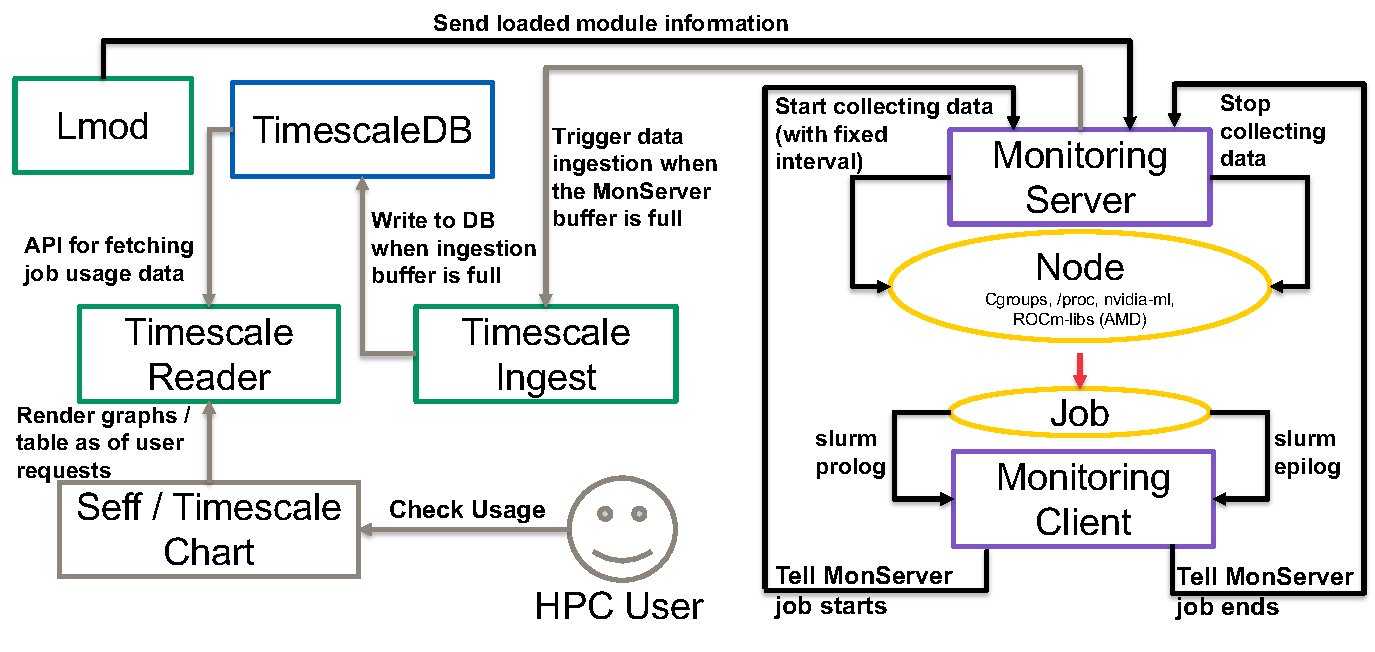
\includegraphics[width=1\textwidth]{figures/monitoring.pdf}
    \caption{Monitoring system structure}
    \label{fig_monitoring}
\end{figure}

\subsection{Monitoring Daemon}

Monitoring Daemon is written in C++ and consists of MonClient and MonServer. MonClient and MonServer are utilities that run on each compute node. They collect the job metadata and metrics and send them out from the node.

MonClient is a CLI utility that passes information about the job start and end to the MonServer process via UDP. MonClient commands are run in prolog and epilog scripts of jobs and tasks in Slurm.

MonServer runs continuously in the background of the compute nodes. It gets information about the job, such as hardware specifications, job ID, and step ID, from the client, collects the metrics of each job accordingly, and sends them to the Timescale Ingest server once the local buffer is complete so we can monitor how the actual hardware resources are used. The metrics that MonServer collects are as follows:

\begin{itemize}
    \item \textbf{CPU usage}: Reads the CPU metrics from \texttt{/proc} for the cores assigned to the job. Since the number of CPU cores can be too large to analyze individual jobs, we can also use the aggregated result of the assigned cores per node.
    \item \textbf{Memory usage per job}: Gets the total memory usage from Cgroups for the job per node. This requires that Slurm is set up to use the Cgroups plugin.
    \item \textbf{Memory usage per process}: Uses the \texttt{ps} command line utility to get the memory usage of processes for a job. \texttt{ps} needs the job step information from prolog and epilog scripts passed by MonClient to get the process ID information.
    \item \textbf{GPU usage}: Reads GPU load, memory, power, temperature, and energy information from Nvidia Management Library / ROCm-SMI for the GPUs assigned to the job.
\end{itemize}

We have intentional delays in collecting the monitoring data to filter out the IO loading period caused by dataset loading and environment initialization so that monitoring can genuinely reflect the use of GPU. Also, those jobs only last for a very short time, so we only collect from those jobs with a meaningful length of data to analyze and reduce the burden of the database and maintain the stability of the whole monitoring infrastructure. Data sent to the Timescale Ingest will be tagged with the job ID, the username, and the step ID if it is for memory usage per process.

We also support dropping those jobs from the collection loop that have exceeded the maximum possible end time configured by the partition or after two weeks in case the job is killed accidentally and the Slurm epilog does not run.


\subsection{Timescale Ingest}

Timescale Ingest offers API for data ingestion through HTTP or UDP. We do symmetric encryption on the monitoring data. We derive a cryptographic key from an API key using the PBKDF2-HMAC-SHA256 (Combining Password-Based Key Derivation Function 2, Hash-based Message Authentication Code, and Secure Hash Algorithm 256-bit), and then use the derived key as the key for AES-GCM (Combining Advanced Encryption Standard and Galois/Counter Mode) encryption. The server is configured to handle incoming data according to the specified protocol. A UDP server is spun up in a separate thread (goroutine in Golang) if UDP is chosen. If HTTP is selected, the server creates a route to handle incoming POST requests to the \textbf{/write} API endpoint. The transmitted data format follows the InfluxDB line protocol \cite{influxlineprotocol}.

We have an ingestion buffer to store the data temporarily in memory. Whenever we receive the data, we parse it into an instance of Go's structs. When the buffer is full, or after a timeout, we sort the buffer by timestamp, convert them into SQL insert statements, and execute them together. This allows us to reduce the database's write load in batches.

Timescale Ingest implements the graceful shutdown, where a Goroutine uses a channel to wait for an interrupt signal (SIGINT or SIGTERM). Once the interrupt signal is received, the server initiates a graceful shutdown process, which involves creating a context with a timeout of 5 seconds, during which the server attempts to finish handling any ongoing requests and stops receiving new updates. The server is forcibly shut down after the timeout or when all requests are completed. Once the server is shut down, any remaining tasks should be completed. This includes closing the database connection, sending all the data in the buffer, and logging.

In addition to the /write API endpoint as demonstrated above, the API design for the Timescale Ingest is as follows:

\begin{itemize}
    \item \textbf{/version}: Displaying the version information and build time. If the current commit is tagged, \texttt{git describe} starts from the tagged commit and counts how many commits are on top of that tag. It then generates a string in the format of \textit{<tag>-<number\_of\_commits>-<short\_commit\_hash>}, where the tag is the name of the closest annotated one reachable from the commit, the number of commits is the count between the tagged commit and the current commit. The short commit hash is the current commit, abbreviated commit hash (typically seven characters).
    \item \textbf{/status}: A JSON-encoded representation of the server's current status, including information about the metrics being ingested. The JSON output contains fields such as \textit{ok} to indicate whether the operation was successful, \textit{msg} to provide any additional messages if the service has any error, and \textit{status} to contain the JSON-encoded heartbeat information with the key as follows:
    \begin{itemize}
        \item \textbf{BufferSize}: The number of metric items currently stored in the buffer.
        \item \textbf{BufferLimit}: The maximum number of metric items allowed in the buffer.
        % \item \textbf{Columns}: A mapping of column names to their respective data types in the data source schema.
        \item \textbf{CommitCount}: The count of commits made to the database.
        \item \textbf{ReceiveCount}: The count of metric items received by the server.
        \item \textbf{NextCommitTime}: The next time scheduled for committing to the database if the buffer is not full.
        \item \textbf{LastCommitDuration}: The duration to commit the last buffer batch to the database.
        \item \textbf{CommitMetric}: The time taken per metric item to commit the last batch to the database.
    \end{itemize}
    \item \textbf{/healthStatus}: A liveliness check for connection status between the ingest and the database.
\end{itemize}

\subsection{TimescaleDB}
TimescaleDB, as the time-series database, introduces a relational aspect to monitoring. This component stores metrics in a structured manner, allowing for complex SQL queries and analysis. TimescaleDB accommodates the evolving nature of HPC workloads by enabling the retention of historical data. It also accelerates the query speed, essential for identifying trends and patterns over time.

Table \ref{tab:gpu_usage} shows how we define the database table for storing the GPU usage data at the job level collected by MonServer. These give us a basic idea of how well the job performs using GPUs.

\begin{table}[H]
    \centering
    \begin{tabular}{|l|l|l|}
        \hline
        Column & Type & Explanation \\
        \hline
        timestamp & TIMESTAMP & Time when the data is collected \\
        host & TEXT & Name of the host where data is from \\
        GPU & INT & ID of the GPU in the host machine \\
        username & TEXT & Name of the user that starts the job \\
        job & INT & ID of the job that uses the GPU \\
        load\_gpu & INT & Instantaneous GPU core load (\%, 0-100) \\
        load\_memory & INT & Instantaneous GPU memory load (\%, 0-100) \\
        used\_mem & BIGINT & Instantaneous GPU memory in use (Byte) \\
        total\_mem & BIGINT & Instantaneous GPU memory in total (Byte) \\
        power & INT & Instantaneous GPU power (mW for Nvidia, uW for AMD) \\
        temperature & INT & Instantaneous GPU temperature (°C for Nvidia, m°C for AMD) \\
        \hline
    \end{tabular}
    \caption{Table for storing GPU usage}
    \label{tab:gpu_usage}
\end{table}

Table \ref{tab:slurm_job_metadata} shows how we define the database table for storing the unstructured job information collected by MonClient. The JSON string in the metadata column represents the data structure containing information related to jobs, tasks, and allocated hardware information. Each JSON object corresponds to a specific event or action within Slurm indicated by the type, such as starting or stopping a job, task, or event. Every type follows a similar structure, containing fields such as \textit{method} (indicating the type of event), \textit{slurmInternalID} (job ID assigned by the Slurm workload manager), \textit{hostname} (name of the computing node), and \textit{gpu\_energy} (energy consumption data for GPUs), which contains the PCI Bus ID of each GPU as well as the energy counter when the event is triggered (in Millijoule, mJ). Here is a breakdown of each unique field of the types that happen in order during a job lifetime:

\begin{table}[H]
    \centering
    \begin{tabular}{|l|l|l|}
        \hline
        Column & Type & Explanation \\
        \hline
        timestamp & TIMESTAMP & Time when the data is collected \\
        host & TEXT & Name of the host where data is from \\
        job & INT & ID of the job that uses the GPU \\
        type & TEXT &  Type of the metadata (start/stop job/task, event) \\
        metadata & TEXT & Actual key-value data in JSON format \\
        \hline
    \end{tabular}
    \caption{Table for storing Slurm job metadata}
    \label{tab:slurm_job_metadata}
\end{table}

\begin{enumerate}
    \item \textbf{start-job} indicates initiating a new job. It includes details such as the user name (\textit{user}), user's ID (\textit{uid}), the group ID that the user belongs to (\textit{gid}), the partition that the job belongs to (\textit{partition}), and resource allocations, e.g., GPU and CPU id lists that get allocated to the job). Additionally, it includes the GPU energy counter of all the GPUs that belong to the node.

\clearpage

\begin{lstlisting}[language=JSON]
{
  "method":"start-job",
  "slurmInternalID":8934,
  "hostname":"g1101",
  "user":"dowjohn",
  "uid":100567,
  "gid":100567,
  "partition":"gputest",
  "gpu":"1",
  "cpu":"0-255",
  "gpu_energy":[
    {
      "pciBusId":"00000000:03:00.0",
      "energy":1260156826
    },
    {
      "pciBusId":"00000000:44:00.0",
      "energy":999985444
    },
    {
      "pciBusId":"00000000:84:00.0",
      "energy":793570107
    },
    {
      "pciBusId":"00000000:C4:00.0",
      "energy":708110133
    }
  ]
}
\end{lstlisting}

    \item \textbf{start-task}: indicates the start of a specific task within a job. It contains metadata such as the task's process ID, step ID (\textit{-1} indicates the batch step), node-local task ID for the process within a job (\textit{locaID}), number of processes in the job step or whole heterogeneous job step (\textit{stepTasks}) and loaded modules, which records the modules name as well as their versions separated by a colon. It also includes the GPU energy counter assigned to the job.

\clearpage

\begin{lstlisting}[language=JSON]
{
  "method":"start-task",
  "slurmInternalID":8934,
  "hostname":"g1101",
  "taskPID":44689,
  "stepID":-1,
  "locaID":0,
  "loadedModules":"gcc/11.2.0:openmpi/4.1.2:openblas/0.3.18-omp:csc-tools:StdEnv",
  "gpu_energy":[
    {
      "pciBusId":"00000000:44:00.0",
      "energy":999996492
    }
  ]
}
\end{lstlisting}

\begin{lstlisting}[language=JSON]
{
  "method":"start-task",
  "slurmInternalID":8934,
  "hostname":"g1101",
  "taskPID":45279,
  "stepID":0,
  "locaID":0,
  "stepTasks":1,
  "loadedModules": "csc-tools:StdEnv:gcc/9.4.0:tensorflow/2.12:openblas/0.3.18-omp:openmpi/4.1.2:cuda/11.5.0",
  "gpu_energy":[
    {
      "pciBusId":"00000000:44:00.0",
      "energy":1000040684
    }
  ]
}
\end{lstlisting}

    \item \textbf{event}: denotes the event that happens when the task is running. This can be that a new module is loaded in the job context.

\begin{lstlisting}[language=JSON]
{
  "method":"event",
  "slurmInternalID":8934,
  "stepID":0,
  "eventKind":"module-load",
  "eventField":"tensorflow/2.15"
}

\end{lstlisting}

    \item \textbf{stop-task}: denotes completing or terminating a task within a job. Like the start task, it includes metadata for the task and the energy consumption of GPUs allocated to the task-related job during its execution.

\begin{lstlisting}[language=JSON]
{
  "method":"stop-task",
  "slurmInternalID":8934,
  "hostname":"g1101",
  "taskPID":44689,
  "stepID":0,
  "locaID":0,
  "stepTasks":1,
  "gpu_energy":[
    {
      "pciBusId":"00000000:44:00.0",
      "energy":1001166893
    }
  ]
}
\end{lstlisting}

\begin{lstlisting}[language=JSON]
{
  "method":"stop-task",
  "slurmInternalID":8934,
  "hostname":"g1101",
  "stepID":-1,
  "locaID":0,
  "gpu_energy":[
    {
      "pciBusId":"00000000:44:00.0",
      "energy":1001173148
    }
  ]
}
\end{lstlisting}

    \item \textbf{stop-job}: indicates the completion or termination of a job. It includes metadata about the job and the total energy consumption of all the GPUs inside the job running node during its execution.

\clearpage

\begin{lstlisting}[language=JSON]
{
  "method":"stop-job",
  "slurmInternalID":8934,
  "hostname":"g1101",
  "gpu":"1",
  "gpu_energy":[
    {
      "pciBusId":"00000000:03:00.0",
      "energy":1261452017
    },
    {
      "pciBusId":"00000000:44:00.0",
      "energy":1001180831
    },
    {
      "pciBusId":"00000000:84:00.0",
      "energy":794875873
    },
    {
      "pciBusId":"00000000:C4:00.0",
      "energy":709266506
    }
  ]
}
\end{lstlisting}

\end{enumerate}

We use TimescaleDB-specific features to improve query performance. We turn the metrics table into a hypertable with 6-hour chunking. We also create indexes on job IDs, hostnames, and GPU IDs, as those are the keys most commonly used for our SQL group queries. We compress data older than one day and drop data older than six months.

We define two triggers and corresponding notification functions in PL/pgSQL -- SQL Procedural language. These triggers are designed to automatically send notifications whenever new data is inserted into table \textit{slurm\_job\_metadata} and \textit{gpu\_usage}.

\clearpage

\begin{lstlisting}[language=SQL]
-- Notify of new job metadata
CREATE OR REPLACE FUNCTION notify_new_job_metadata_insertion()
  RETURNS trigger AS $notify_new_job_metadata_insertion$
BEGIN
  PERFORM pg_notify('job_updates', (NEW.host || '|' || NEW.job || '|' || NEW.type || '|' || NEW.metadata)::text);
  RETURN NEW;
END;
$notify_new_job_metadata_insertion$ LANGUAGE plpgsql;

CREATE TRIGGER job_metadata_insertion_notify_trigger
AFTER INSERT ON slurm_job_metadata
FOR EACH ROW EXECUTE FUNCTION notify_new_job_metadata_insertion();

-- Notify on new gpu_usage_aggregate data
CREATE OR REPLACE FUNCTION notify_new_gpu_usage_insertion()
  RETURNS trigger AS $notify_new_gpu_usage_insertion$
BEGIN
  PERFORM pg_notify('gpu_usage_insertion', (NEW.host || ',' || NEW.gpu || ',' || NEW.job || ',' || NEW.load_gpu || ',' || NEW.load_memory || ',' || NEW.used_mem || ',' || NEW.power || ',' || NEW.temperature)::text);
  RETURN NEW;
END;
$notify_new_gpu_usage_insertion$ LANGUAGE plpgsql;

CREATE TRIGGER gpu_usage_insertion_notify_trigger
AFTER INSERT ON gpu_usage
FOR EACH ROW EXECUTE FUNCTION notify_new_gpu_usage_insertion();
\end{lstlisting}


\begin{itemize}
    \item \textbf{notify\_new\_job\_metadata\_insertion()}: This function retrieves the newly inserted row and constructs a notification message using concatenation (\textit{||}) separated with \textit{|} to avoid any collision with the JSON format text (metadata). The message includes all the fields except the timestamp from the inserted row. Finally, the \textit{pg\_notify()} function is called to send a notification to a specific channel named \textit{job\_updates}.
    \item \textbf{job\_metadata\_insertion\_notify\_trigger}: This trigger fires after each insertion into the \textit{slurm\_job\_metadata} table. It is associated with the \\
    \textit{notify\_new\_job\_metadata\_insertion()} function, causing the function to execute automatically whenever new data is inserted into the table.
    \item \textbf{notify\_new\_gpu\_usage\_insertion()}: Similar to the first function, it constructs a notification message using all the fields except the timestamp, username, and total\_mem from the inserted row separated by commas (\textit{,}). It then notifies through the \textit{gpu\_usage\_insertion} channel.
    \item \textbf{gpu\_usage\_insertion\_notify\_trigger}: This trigger fires after each insertion into the \textit{gpu\_usage} table and is associated with the \textit{notify\_new\_gpu\_usage\_insertion()} function, triggering it automatically upon insertion of new data.
\end{itemize}

These triggers and notification functions facilitate real-time communication within the database system. They enable other parts of the system to be notified instantly whenever new job metadata or GPU usage data is inserted, allowing for timely updates and actions based on the newly inserted data.

\subsection{Timescale Reader}
The Timescale Reader component facilitates the retrieval of metrics from TimescaleDB for analysis and reporting. It provides a RESTful API for building other elements that support administrators in gaining insights into historical resource utilization, aiding in capacity planning, performance optimization, and trend analysis. It also enables the integration of other components to show statistics to users via GUI or CLI. The Timescale Reader complements the real-time monitoring capabilities, providing a comprehensive view of metrics across different time intervals.

We have a centralized web page that allows users to use the APIs provided by Timescale Reader to check job history data with interactive graphs about the GPU load, memory, power, and temperature, as shown in Figure \ref{fig_gpu-usage-history-dashboard}. Figure \ref{fig_gpu-usage-graph} shows one example of a graph rendered via Timescale Chart through Timescale Reader API data. It also has accessibility support to help viewers with vision deficiencies (e.g., color blindness or partial sight) more easily understand the data with patterns and gradients, as shown in Figure \ref{fig_gpu-usage-graph-accessibility}.

\begin{figure}[H]
    \centering
    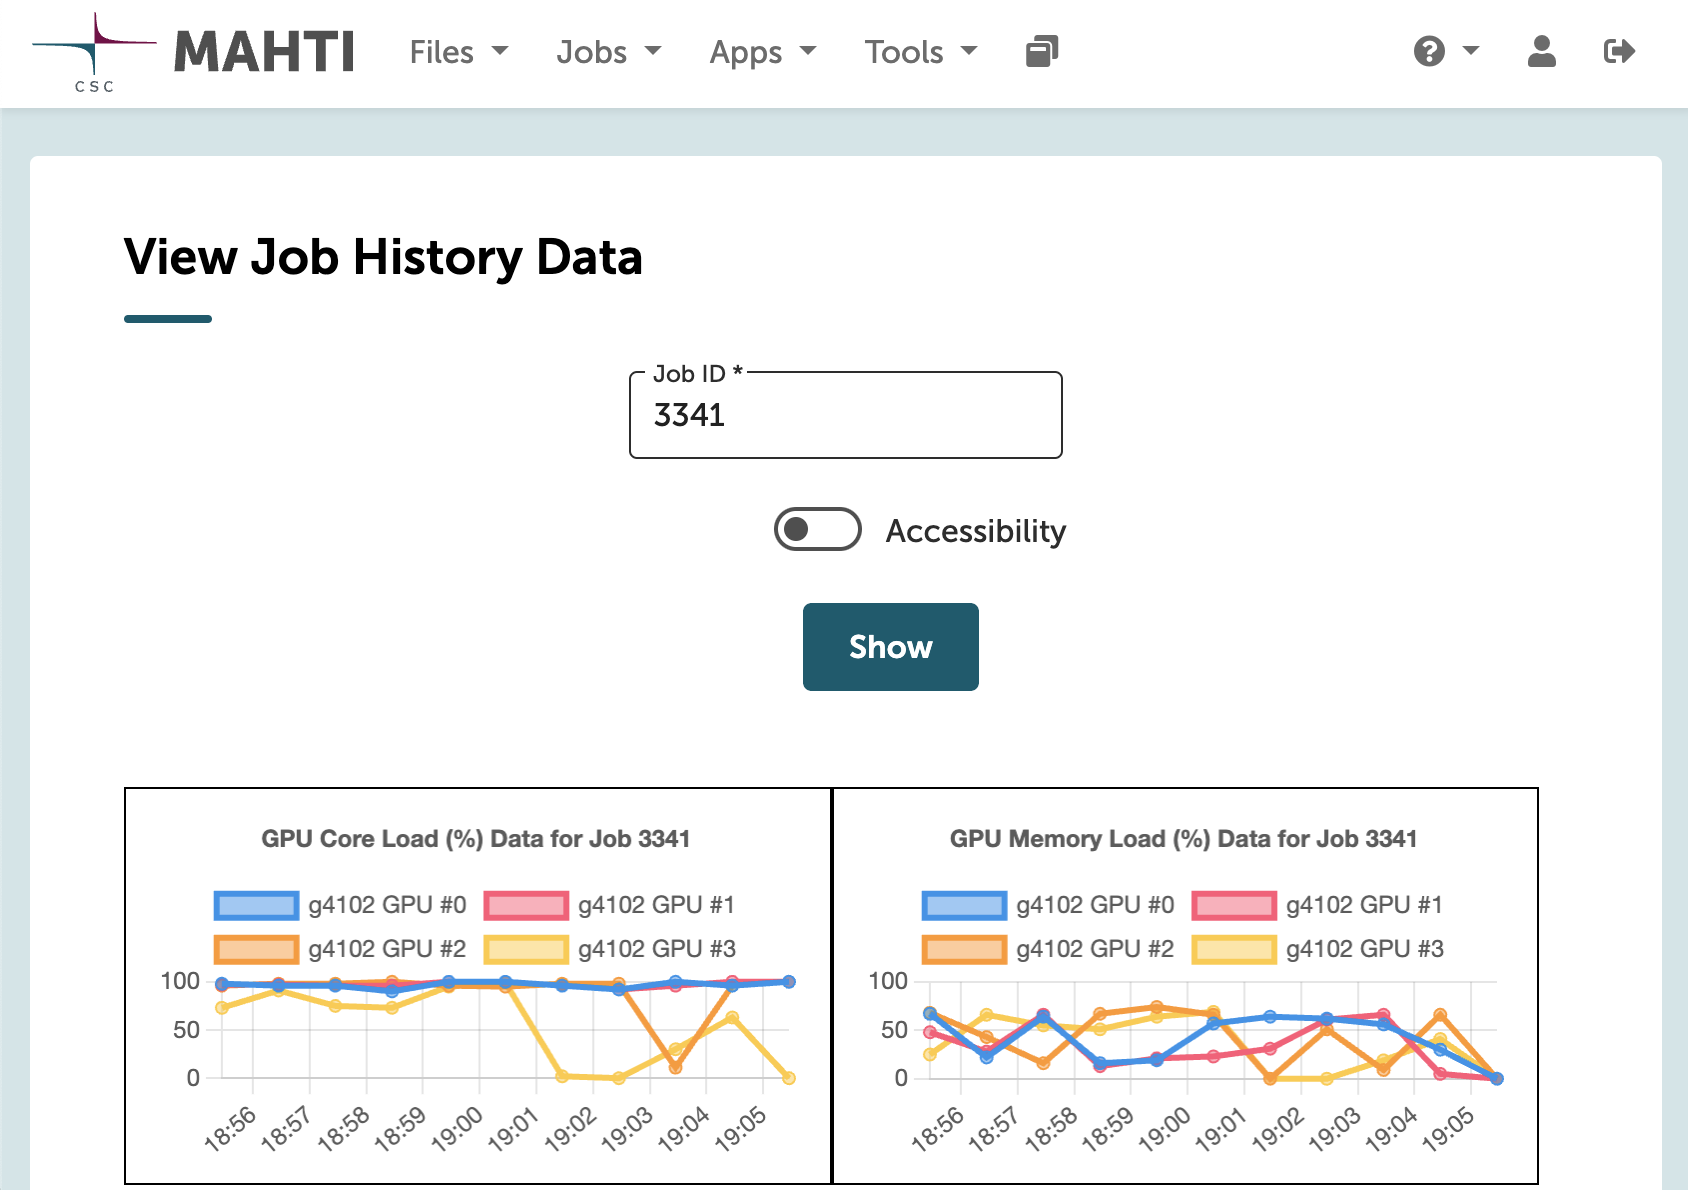
\includegraphics[width=1\textwidth]{figures/data-dashboard.png}
    \caption{GPU usage history checking dashboard}
    \label{fig_gpu-usage-history-dashboard}
\end{figure}

\begin{figure}[H]
    \centering
    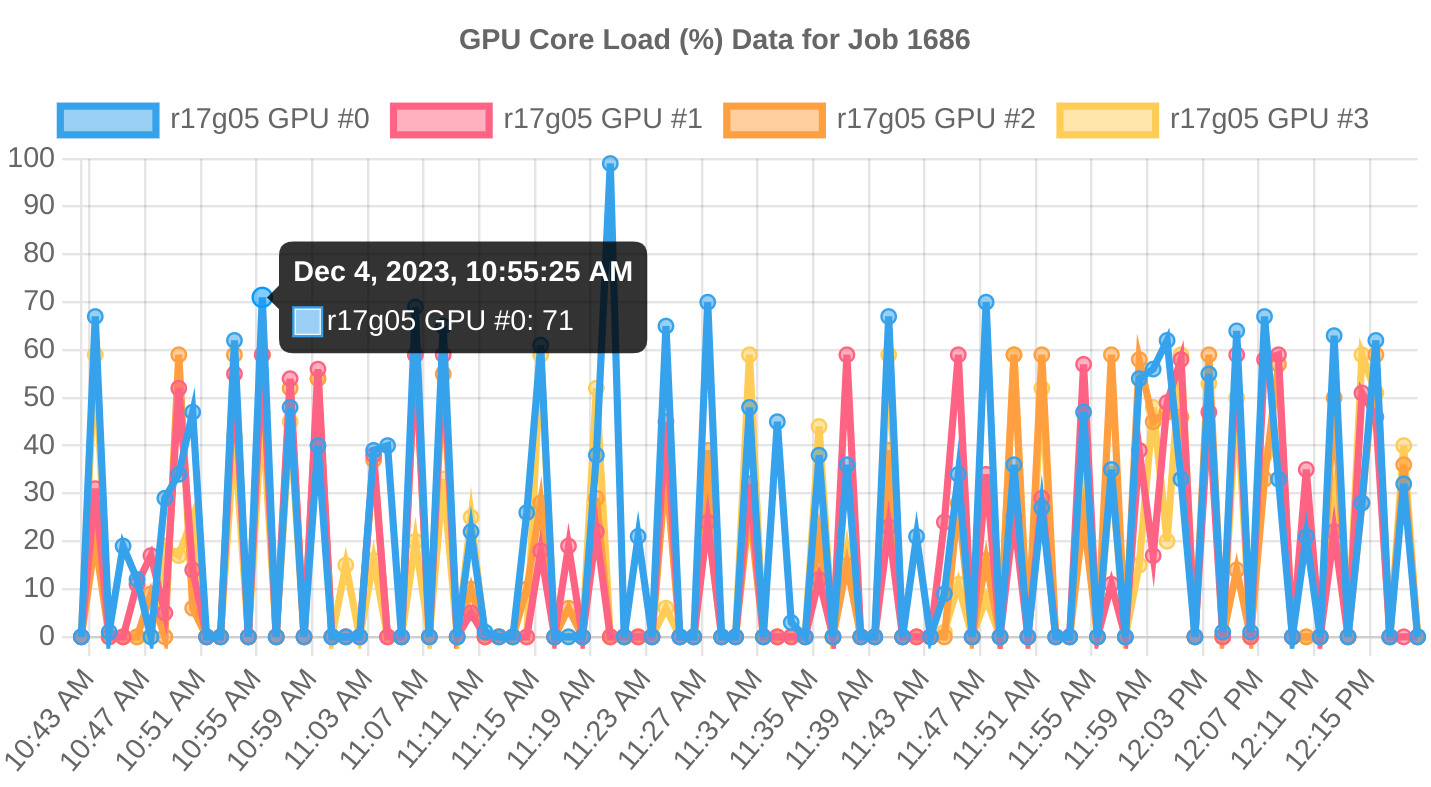
\includegraphics[width=1\textwidth]{figures/usage-graph.png}
    \caption{GPU usage history graph from Timescale Chart}
    \label{fig_gpu-usage-graph}
\end{figure}

\begin{figure}[H]
    \centering
    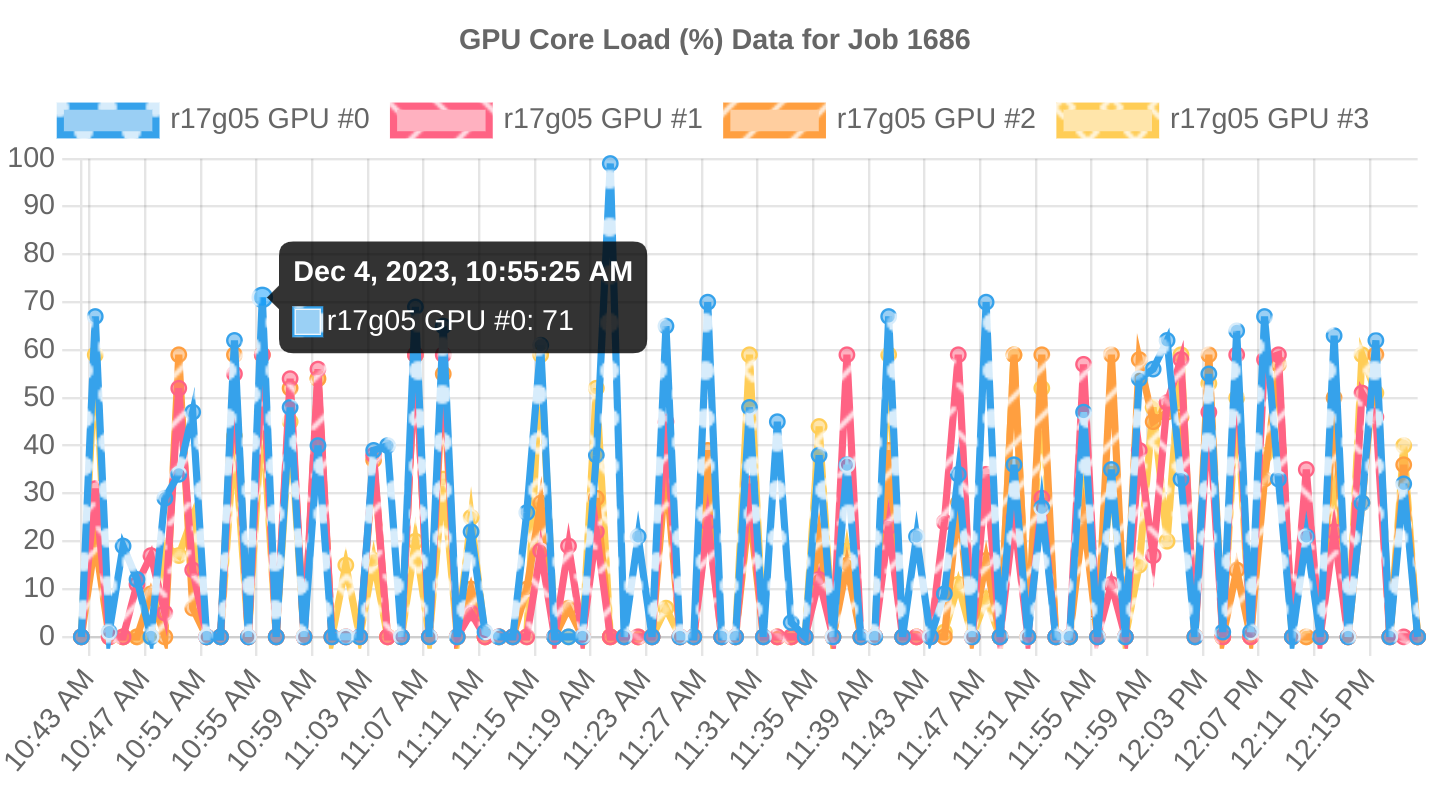
\includegraphics[width=1\textwidth]{figures/usage-accessibility-graph.png}
    \caption{GPU usage history graph from Timescale Chart with accessibility}
    \label{fig_gpu-usage-graph-accessibility}
\end{figure}

Below is an example showing the output of our modified \textit{seff} command. The GPU job efficiency section is printed via the Timescale Reader API. Here, we show the metrics related to the GPU, including the load, memory, and energy. Each entry shows the hostname, the GPU ID about the metrics, and the aggregated mean, standard deviation, and maximum value for the whole job history.

\clearpage

\begin{lstlisting}
$ seff 5465
Job ID: 5465
Cluster: mahti
User/Group: johndoe/pepr_johndoe
State: COMPLETED (exit code 0)
Nodes: 1
Cores per node: 16
CPU Utilized: 19-19:45:45
CPU Efficiency: 82.58% of 24-00:05:52 core-walltime
Job Wall-clock time: 1-12:00:22
Memory Utilized: 14.41 GB
Memory Efficiency: 22.51% of 64.00 GB
Job consumed 3600.61 CSC billing units based on the following used resources.
Billed project: project_1008888
Non-Interactive BUs: 3600.61
GPU BU: 7201.22
NVME BU: 38.89
GPU job efficiency:
-------------------------------------------------------------------
GPU load
    Hostname      GPU Id      Mean (%)    stdDev (%)       Max (%)
       g5101           0         86.21         18.69         99.00
       g5101           3         78.53         19.65         97.00
-------------------------------------------------------------------
GPU memory
    Hostname      GPU Id    Mean (GiB)  stdDev (GiB)     Max (GiB)
       g5101           0         22.64          0.00         22.64
       g5101           3         22.32          0.00         22.33
-------------------------------------------------------------------
GPU energy
    Hostname      GPU Id   Energy (Wh)
       g5101           0       8532.60
       g5101           3       8664.34
-------------------------------------------------------------------
\end{lstlisting}

The API design for the Timescale Reader is as follows:

\begin{itemize}
    \item \textbf{/version}: Same as Timescale Ingest, it displays the version information and build time.
    \item \textbf{/status}: Liveness checking endpoint.
    \item \textbf{/chart}: Serving the static files for Timescale Chart JS web interface (an encapsulated web component using Chart.js), available parameters can be referred from Table \ref{tab:chart_params}.
    \item \textbf{/getJobs}: Endpoint for listing all the available job IDs in the database with valid GPU monitoring data, meaning those jobs are long enough to view data.
    \item \textbf{/getData/:table/:jobid}: Fetching the raw (unaggregated) history data in JSON format to be rendered by Timescale Chart.
    \item \textbf{/getLoad/:metric/:resource/:jobid/:type}: Displaying aggregated result of the history monitoring data.
    \item \textbf{/getGPUEnergy/:jobid}: Displaying the GPU energy counter.
\end{itemize}


\begin{table}[H]
\centering
\caption{Timescale Chart parameter description}
\begin{tabular}{|l|p{10cm}|}
\hline
\textbf{Parameter} & \textbf{Description} \\ \hline
api & API endpoint to read data from, such as \texttt{http://localhost:8001/getData}. Default to be \texttt{/getData} at the same site. \\ \hline
domain & Database table name to read from, such as \texttt{gpu\_usage}. \\ \hline
job & Job ID to be displayed. \\ \hline
title & Title of the chart. \\ \hline
group & Grouping of the data for different domain datasets, such as \texttt{core} (for \texttt{CPU usage}), \texttt{gpu} (for \texttt{GPU usage}), \texttt{pid} (for \texttt{Memory usage by PID}). \\ \hline
metric & Column name of the data to be displayed in the specific table. \\ \hline
name & Name of the group that will be displayed. \\ \hline
divide & Value to divide the data with. \\ \hline
mode & Chart zoom and pan mode, available values are \texttt{xy}, \texttt{x}, \texttt{y}. The default is \texttt{x}, which means zoom only at the x-axis. \\ \hline
type & Chart graph type, default is \texttt{line} \\ \hline
\end{tabular}
\label{tab:chart_params}
\end{table}

The parameters we support for displaying the aggregated result of the history monitoring data, as well as the GPU energy counter, are as follows:

\begin{itemize}
    \item \textbf{display}: 1 for printing in human-readable format, 2 for printing a table (similar to human-readable format but separated by tabs), and any other values will be in JSON format organized by a list of values using the hostname as the top level and hardware ID as the second level.
    \item \textbf{unit}: Specify the unit of the value to be printed.
    \item \textbf{type}: Specify the name of the value.
    \item \textbf{metric}: Specify the metric of the value (average, minimum, maximum, standard deviation, etc.), support multiple metrics separated by \textit{,} (comma).
    \item \textbf{divide}: Divide the data value stored in the database by this specified number.
    \item \textbf{precision}: Specify the precision of the value to be printed. The default is 2. -1 for no rounding.
    \item \textbf{index}: Specify the device's index to get printed. The default is all devices.
    \item \textbf{hide\_device}: 1 for hiding the \texttt{[device]}, other values for printing the \texttt{[device]}.
\end{itemize}

The human-readable printing format is as follows. Note that \#[\text{index}] will only get printed when there is more than one.

\begin{equation*}
[\text{device}]~\#[\text{index}]~([\text{type}] \ [\text{metric}]):~[\text{value}] \ [\text{unit}]
\end{equation*}


\section{Alert algorithms}
\label{sec:algo_method}
The Alert algorithms component comprises predefined algorithms, that determine the conditions under which alerts are triggered. These algorithms consider various factors, including GPU utilization thresholds and temperature limits. The flexibility of the alert algorithms allows for customization --- based on the specific requirements of HPC clusters --- ensuring that alerts are triggered for conditions deemed critical by administrators.

Regarding the design of the alert algorithms for GPU usage: many high-performance computing applications have load-balancing issues regarding pipeline parallelism, and the data has highly fluctuated characteristics for multiple GPU jobs. Thus, alerting only according to average is neither reliable nor practical, as it may not be fixable easily by the user, so those can be non-critical. Machine learning models could be one way to address the data fluctuation issue by recognizing the data pattern. Algorithm \ref{algo:ml} defines how we can use them.

\begin{algorithm}[H]
\SetAlgoLined
\KwData{Array, Fixed-size sliding window of latest GPU usage history: $A$}
\KwResult{Boolean, indicating if an alert should be raised}
\SetKwFunction{FMain}{checkAlert}
\SetKwFunction{FML}{mlAlgo}
\SetKwProg{Fn}{Function}{:}{}

\Fn{\FML{$array$}}{
    Run a machine learning algorithm with an input of $array$\;
    \Return classification result (0 or 1) for good or bad jobs\;
}

\Fn{\FMain{$A$}}{
    $R \leftarrow \FML(A)$\;
    \If{$R == 1$}{
        \Return true\;
    }
    \Else{
        \Return false\;
    }
}

\caption{Checking GPU load alert based on machine learning}
\label{algo:ml}
\end{algorithm}

Unsupervised machine learning, such as reinforcement learning, is hard to train and interpret. Deep learning algorithms are also very slow to run, and do not fit our need for real-time job analysis. Most importantly, we cannot find a good reward function. The only way is from human feedback.

For supervised machine learning, such as random forests that involve decision trees, although it can be much faster to run, all the data collected from the monitoring system is unlabeled. It is unrealistic for humans to label all those data manually.

In the hope of doing labeling automatically, we also did the silhouette analysis of K-means clustering on the collected GPU monitoring data starting from December 2023 directly, as shown in Figure \ref{fig_silhouette_directly}, as well as features generated with statistical aggregation, as shown in Figure \ref{fig_silhouette_statistics}. Each color in the figure represents a cluster. The red vertical line denotes the average silhouette coefficient value across all clusters. More explanation of silhouette analysis can be found in Subsection \ref{subsec:silhouette}. The result shows that neither of the methods works well since most clusters have the majority proportion of negative coefficient value, and they cannot be reasonable classifications. 

\begin{figure}[H]
    \centering
        \subfloat[n\_clusters = 2]{
        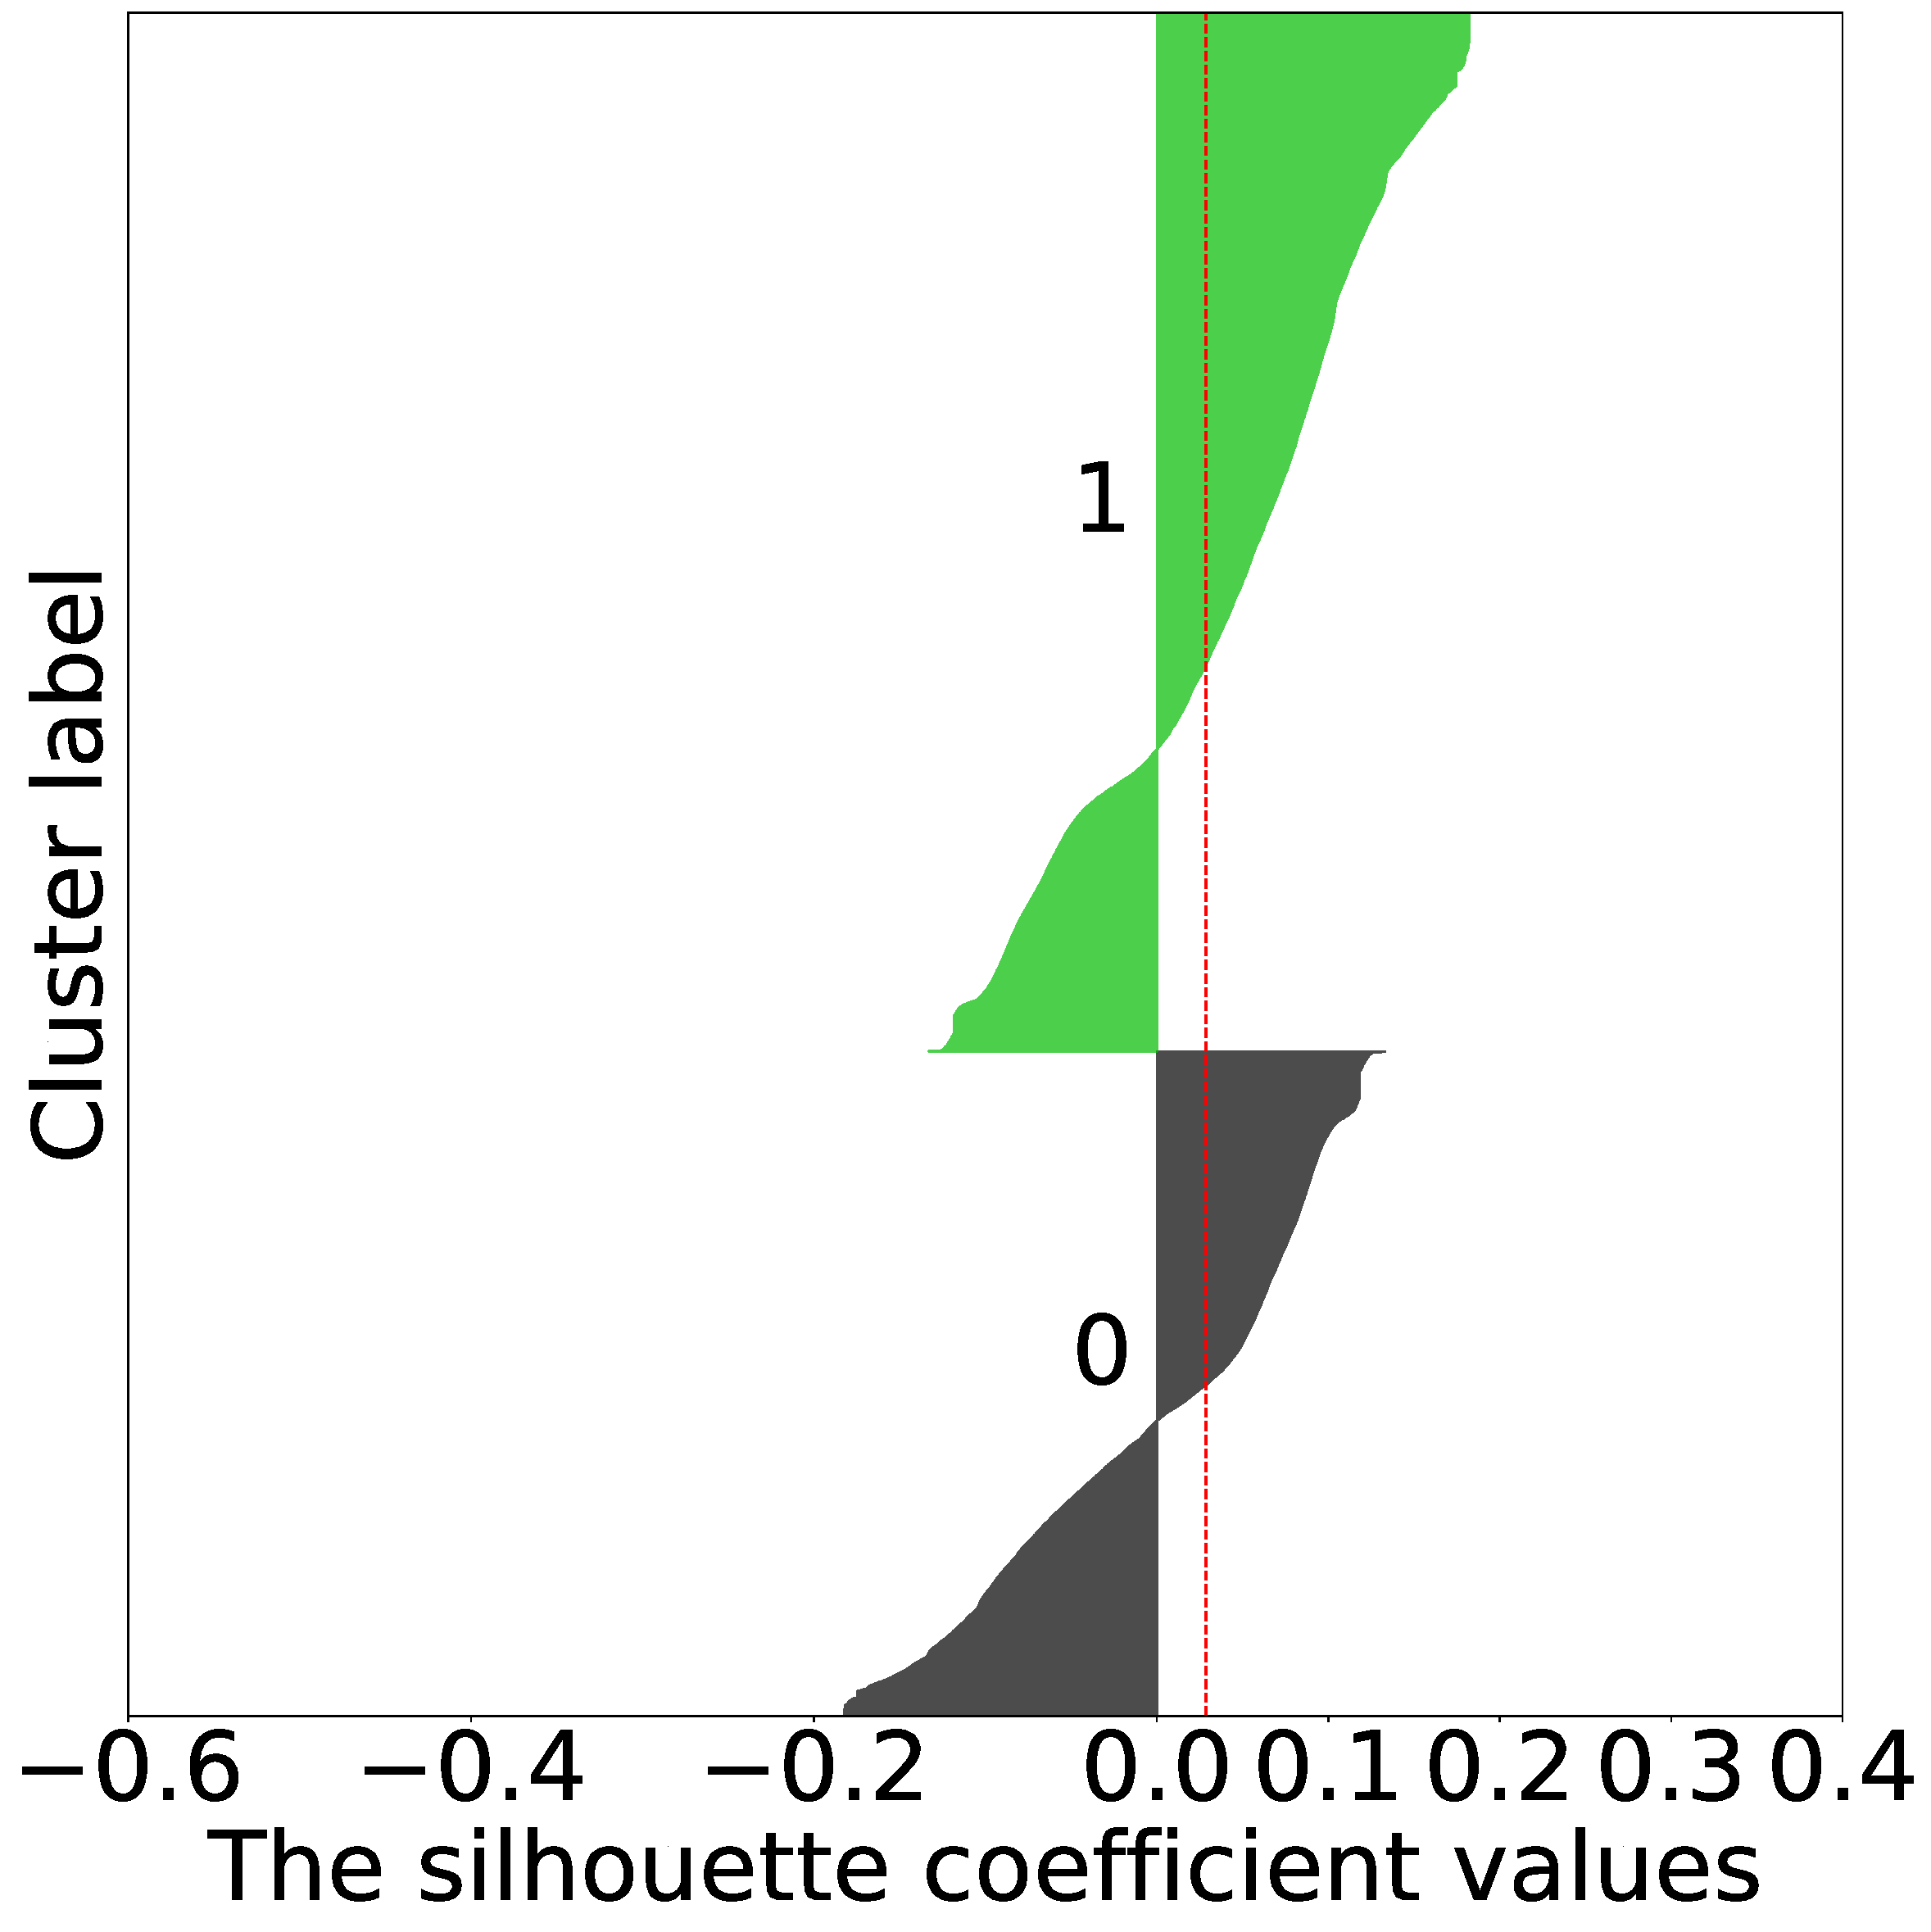
\includegraphics[width=0.45\textwidth]{figures/silhouette/silhouette_directly_2.pdf}
    }
        \subfloat[n\_clusters = 3]{
        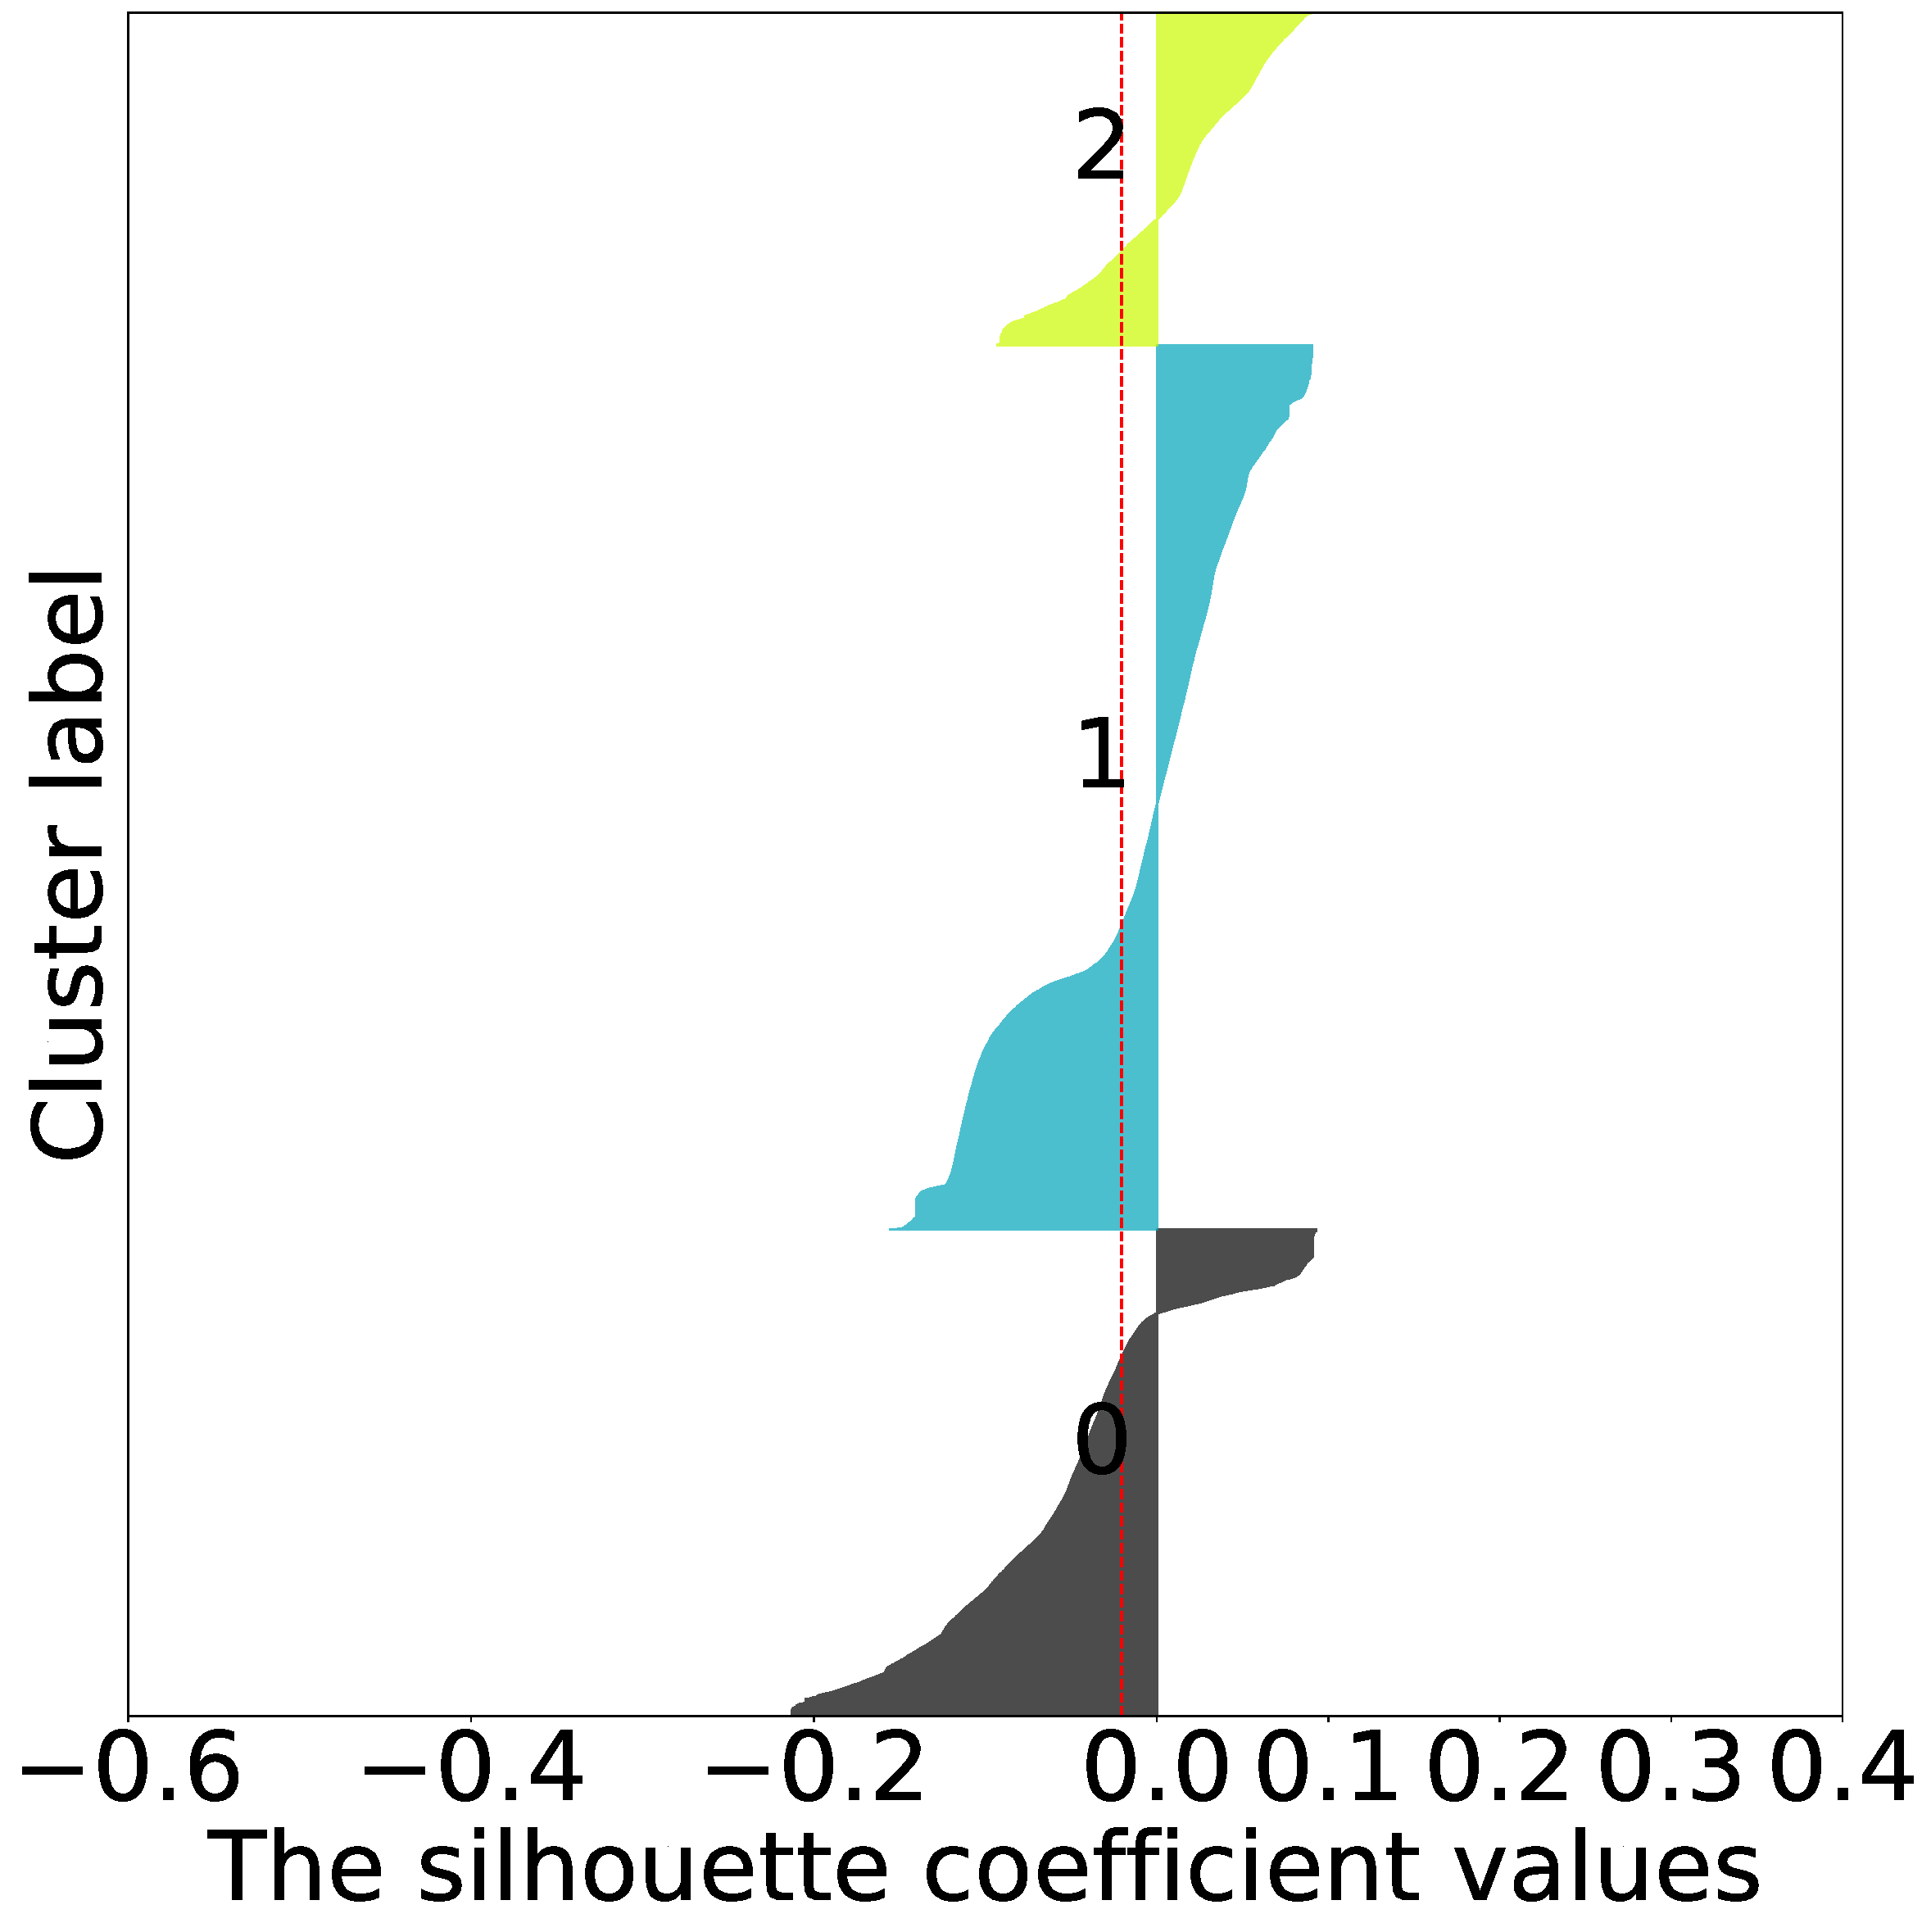
\includegraphics[width=0.45\textwidth]{figures/silhouette/silhouette_directly_3.pdf}
    }\\
        \subfloat[n\_clusters = 4]{
        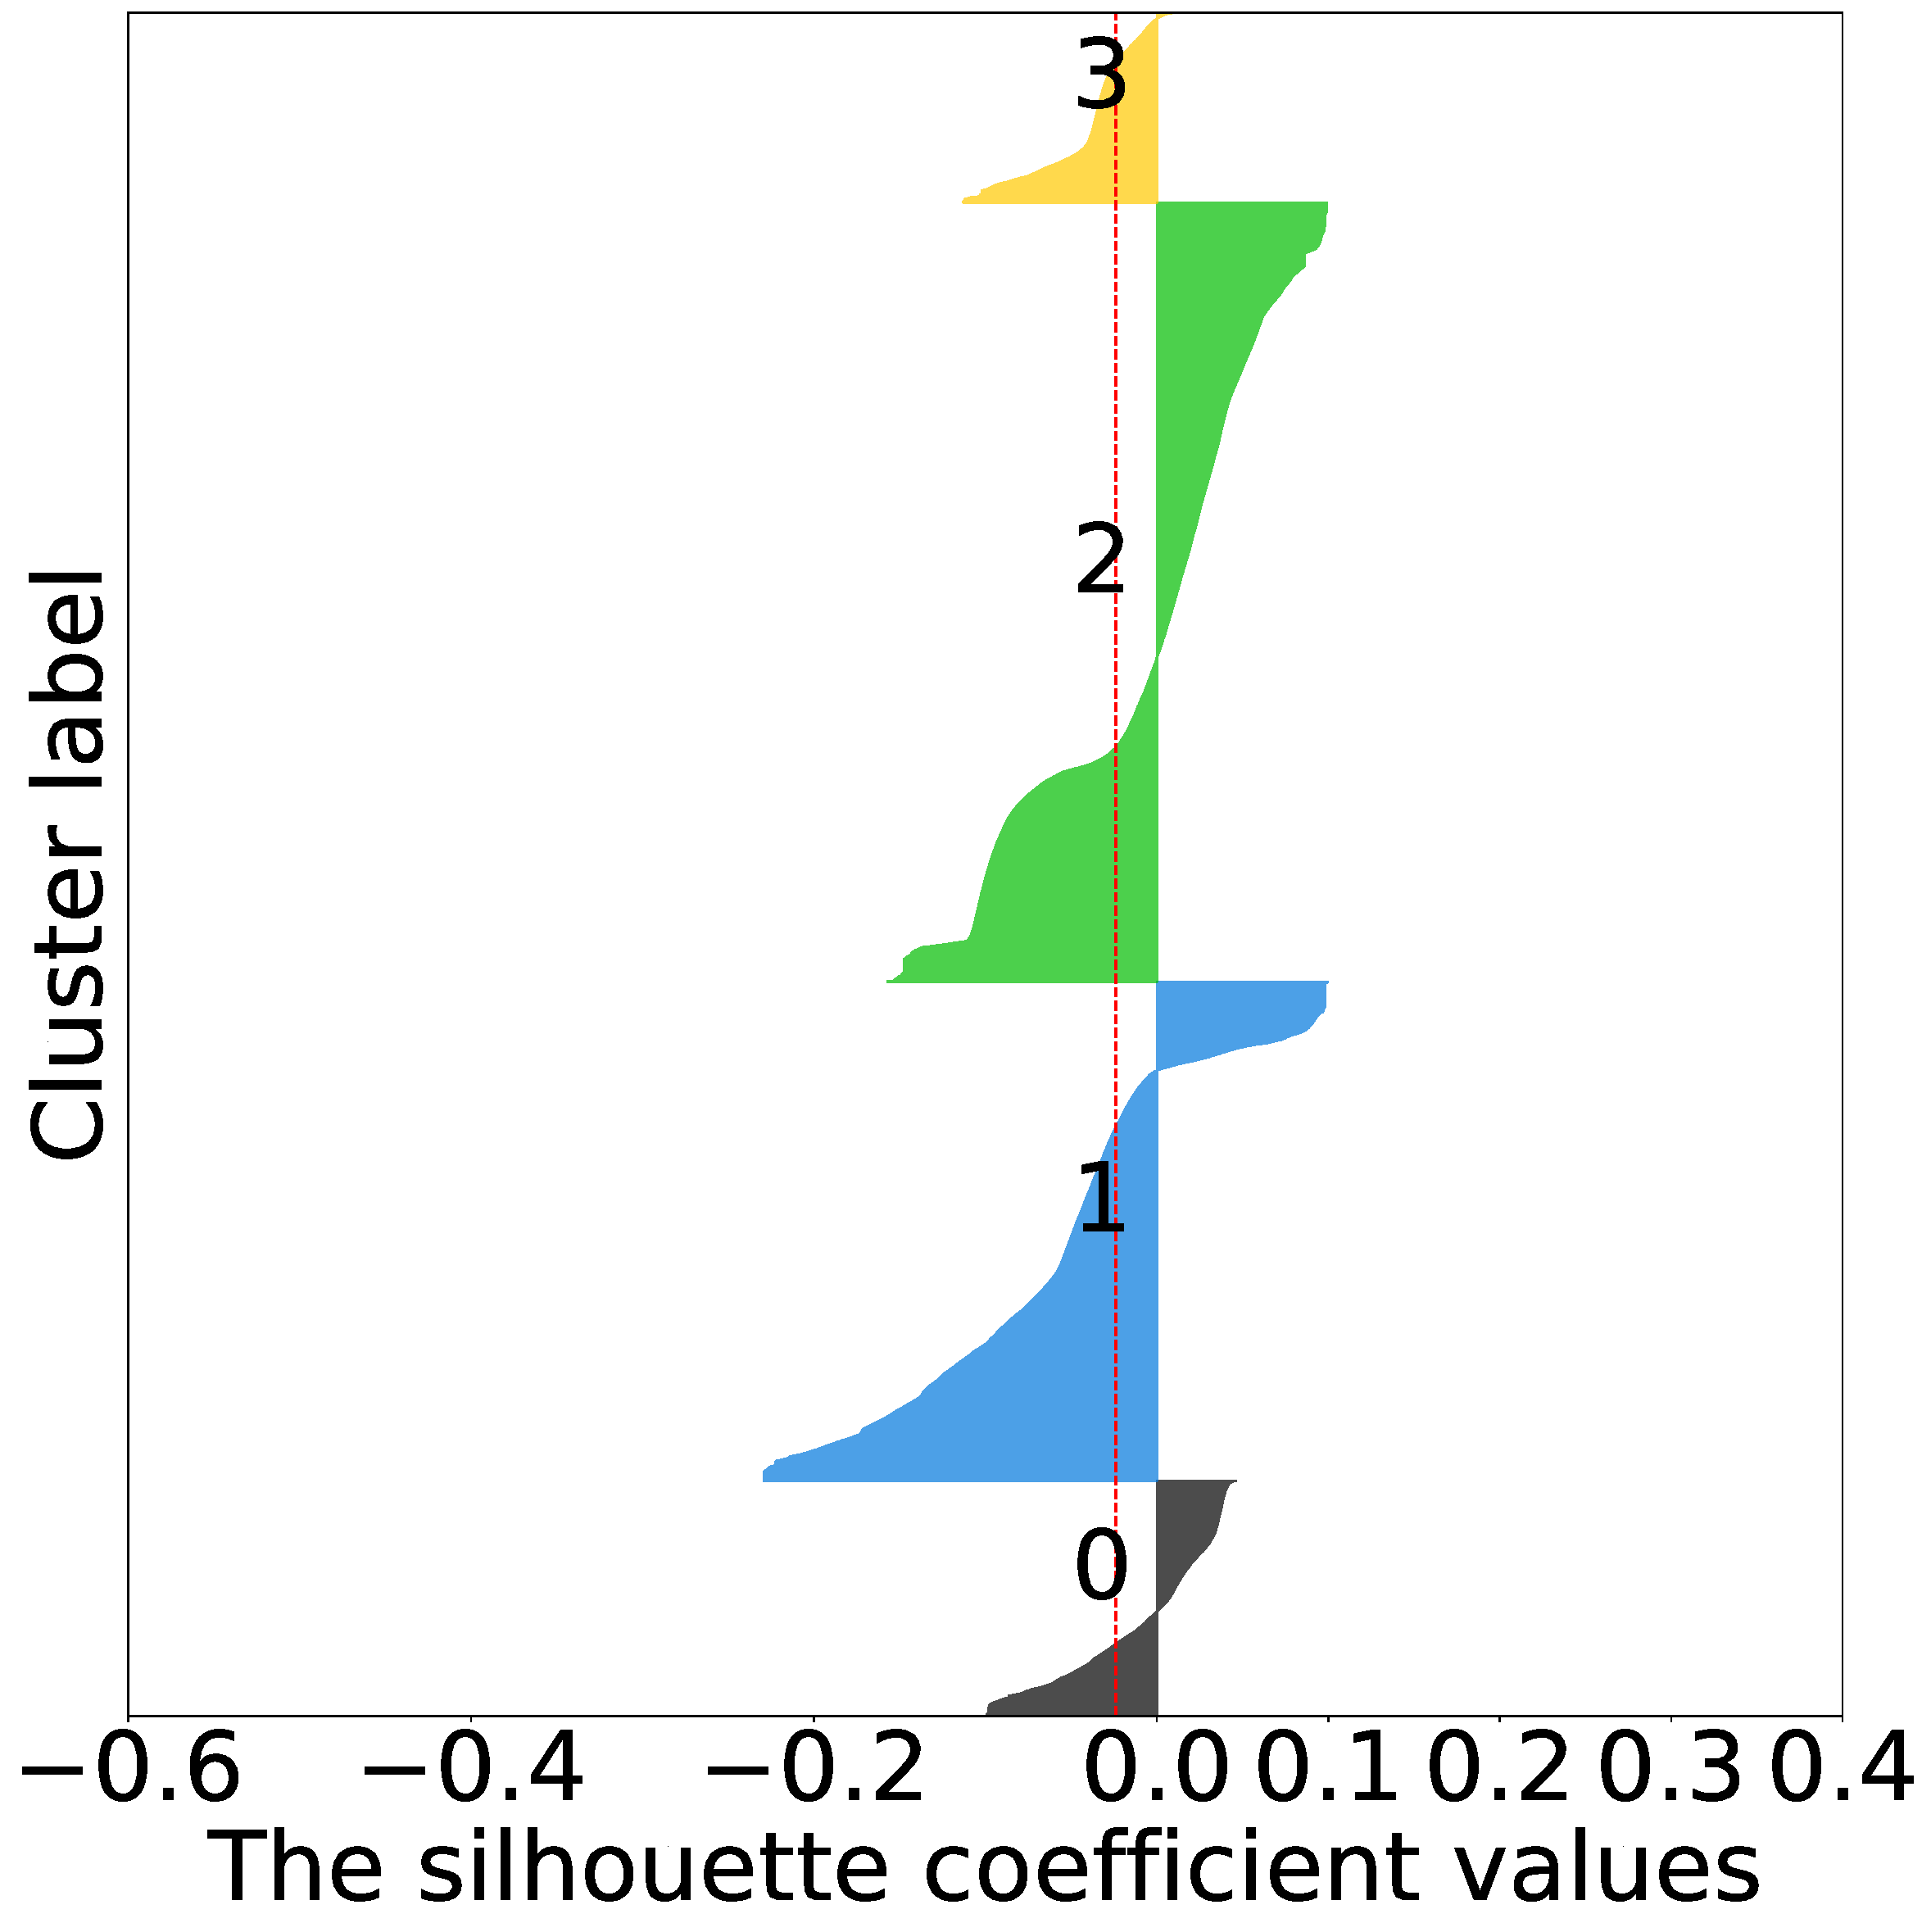
\includegraphics[width=0.45\textwidth]{figures/silhouette/silhouette_directly_4.pdf}
    }
        \subfloat[n\_clusters = 5]{
        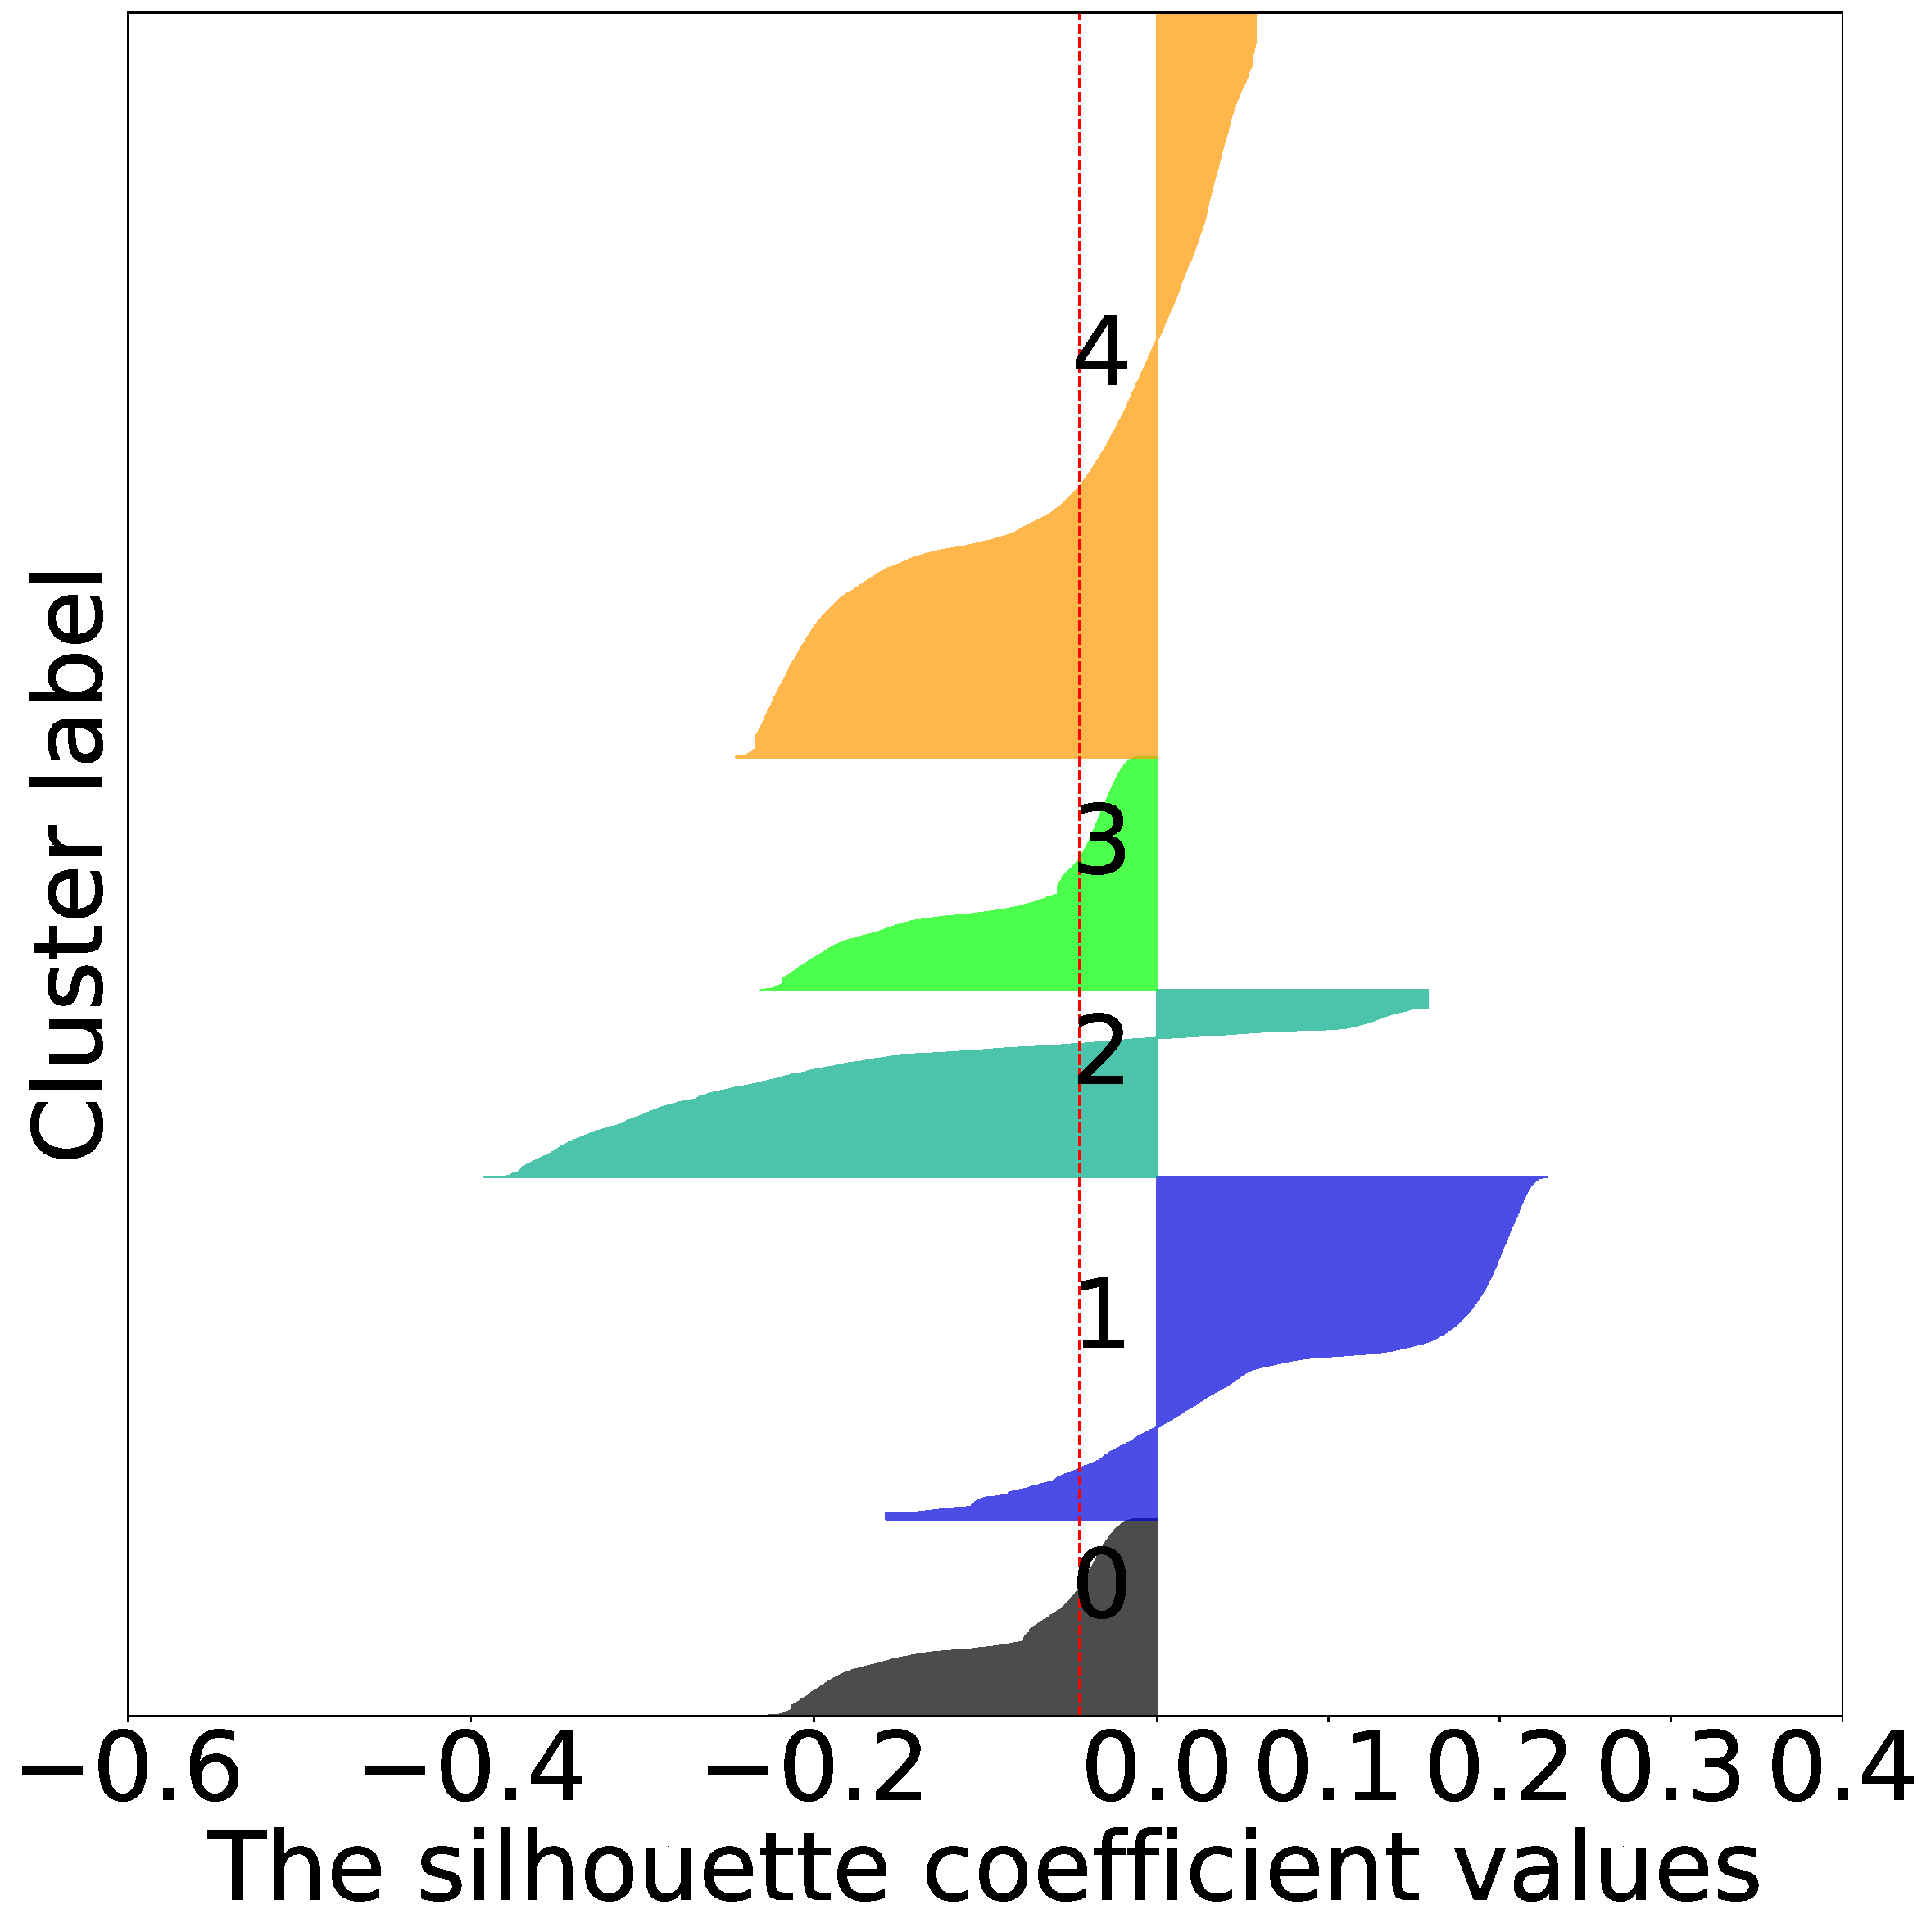
\includegraphics[width=0.45\textwidth]{figures/silhouette/silhouette_directly_5.pdf}
    }\\
        \subfloat[n\_clusters = 6]{
        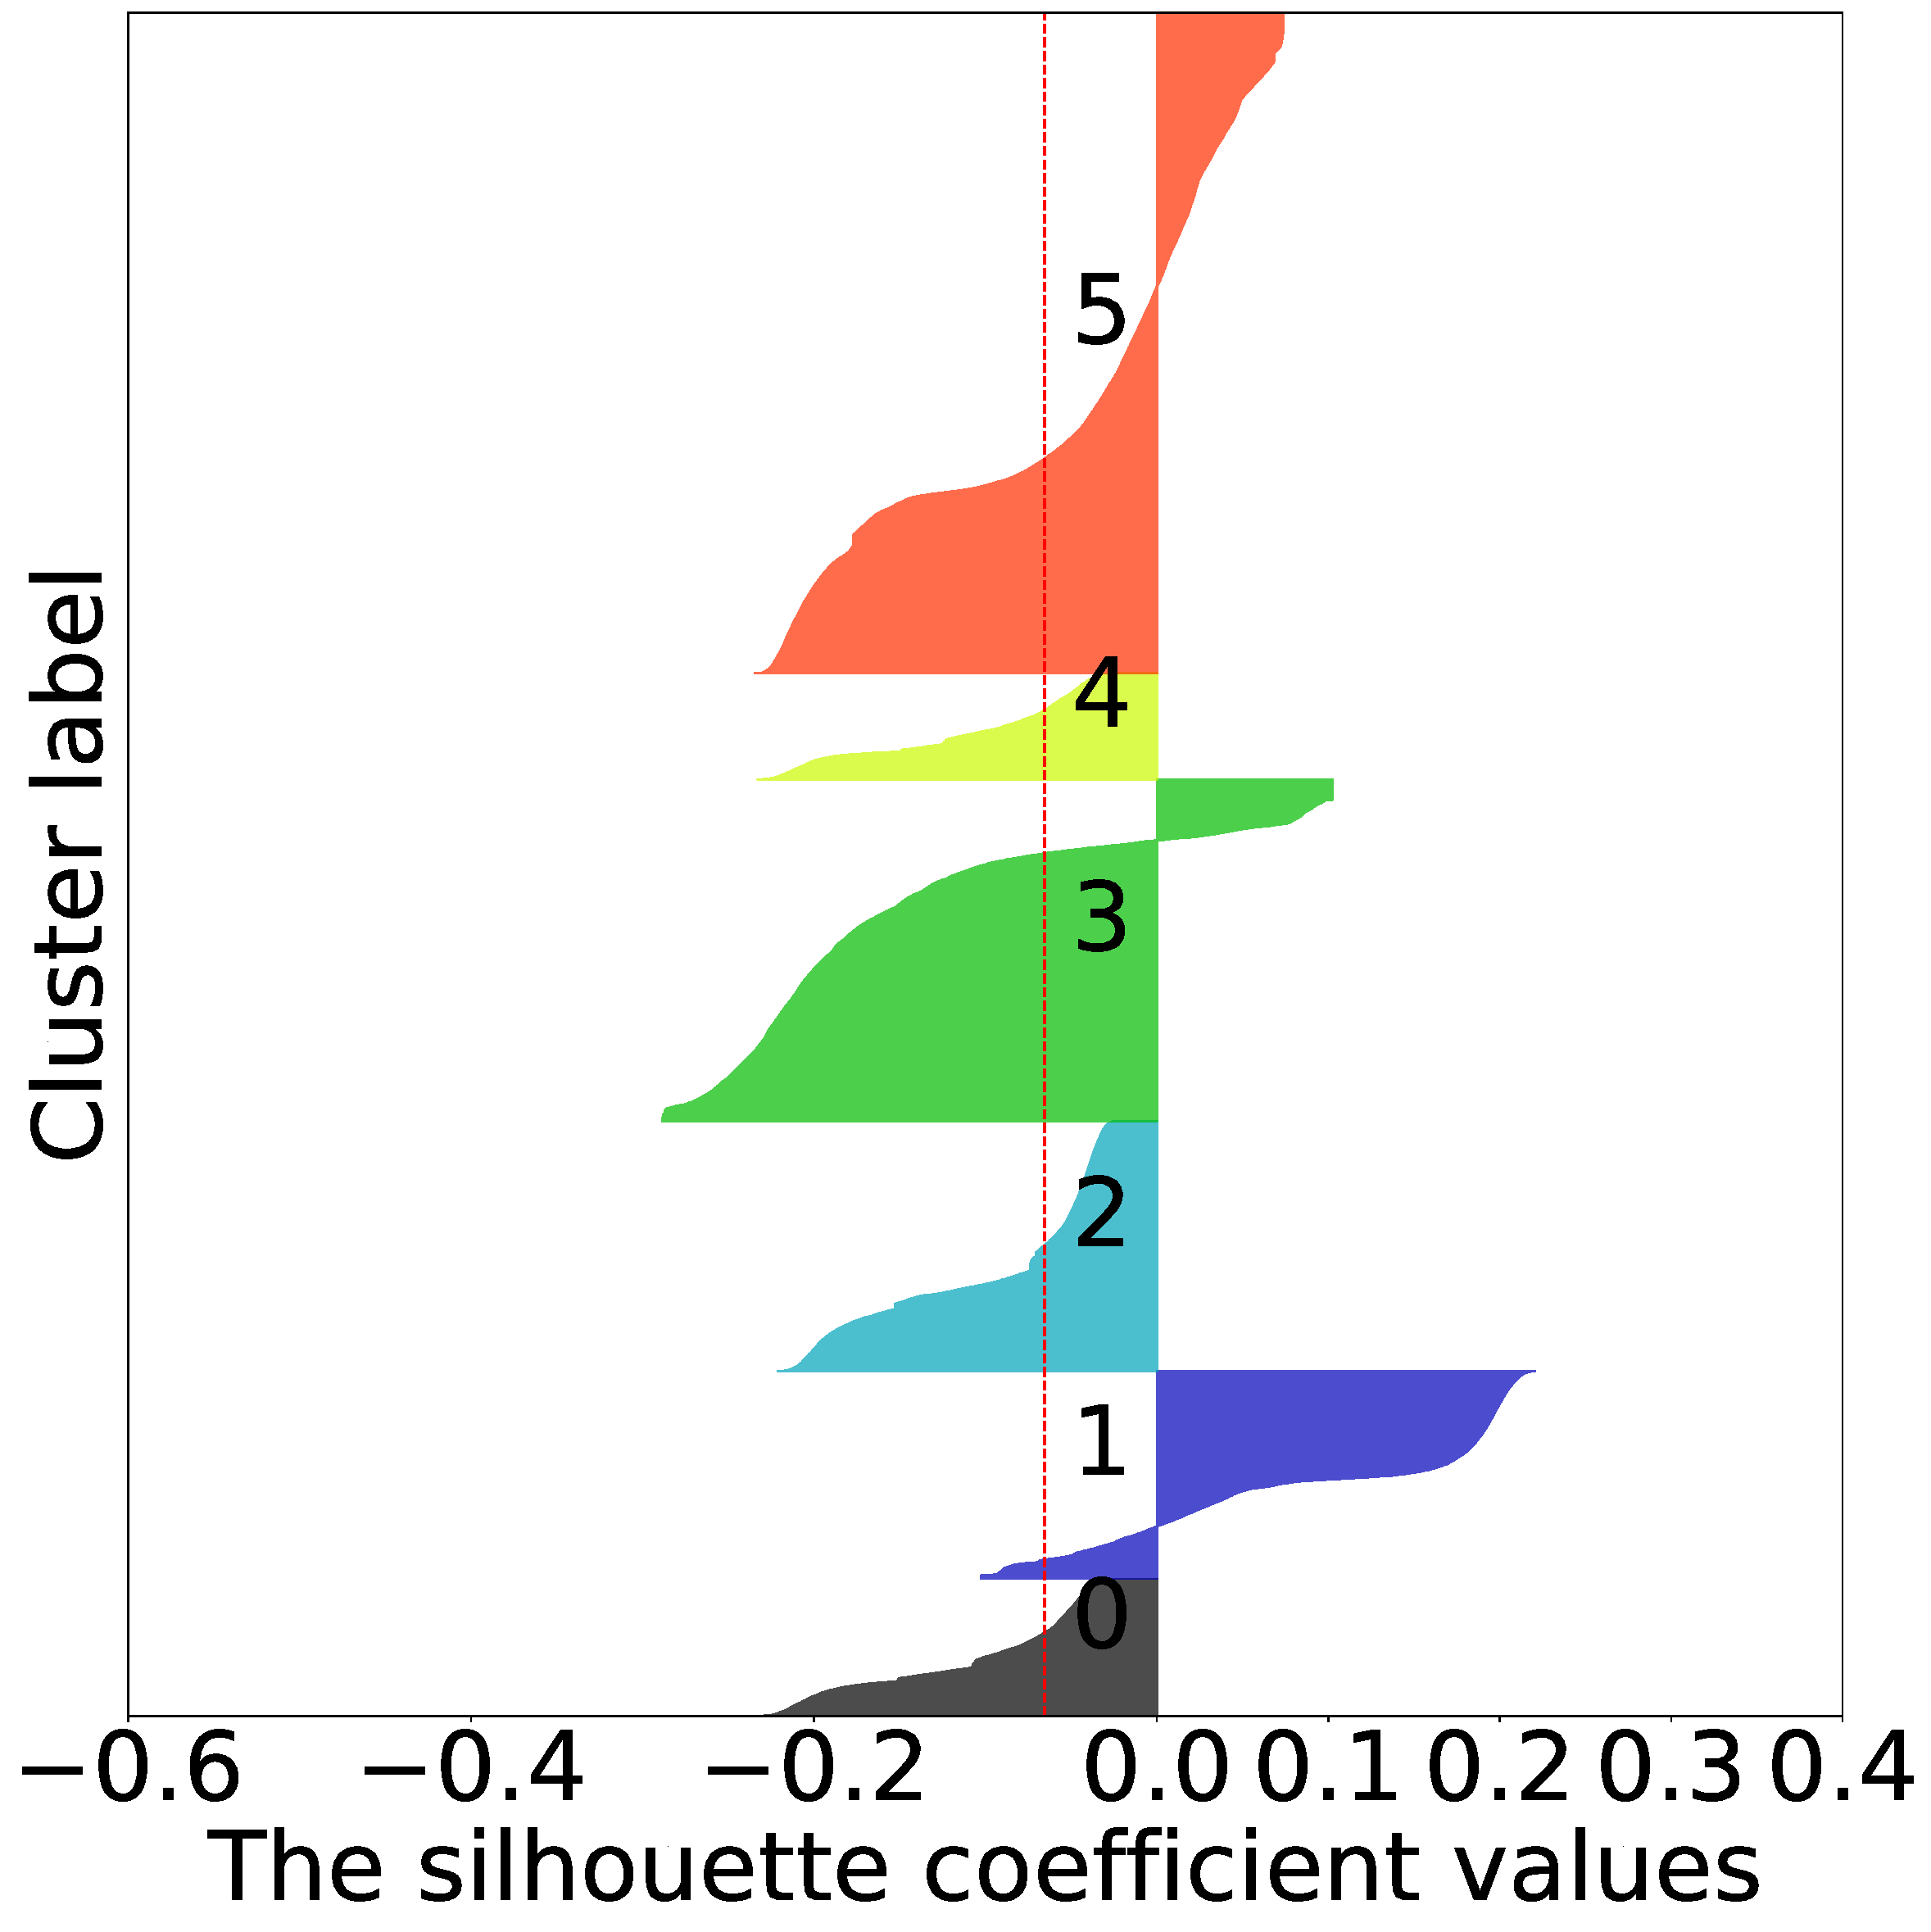
\includegraphics[width=0.45\textwidth]{figures/silhouette/silhouette_directly_6.pdf}
    }
        \subfloat[n\_clusters = 7]{
        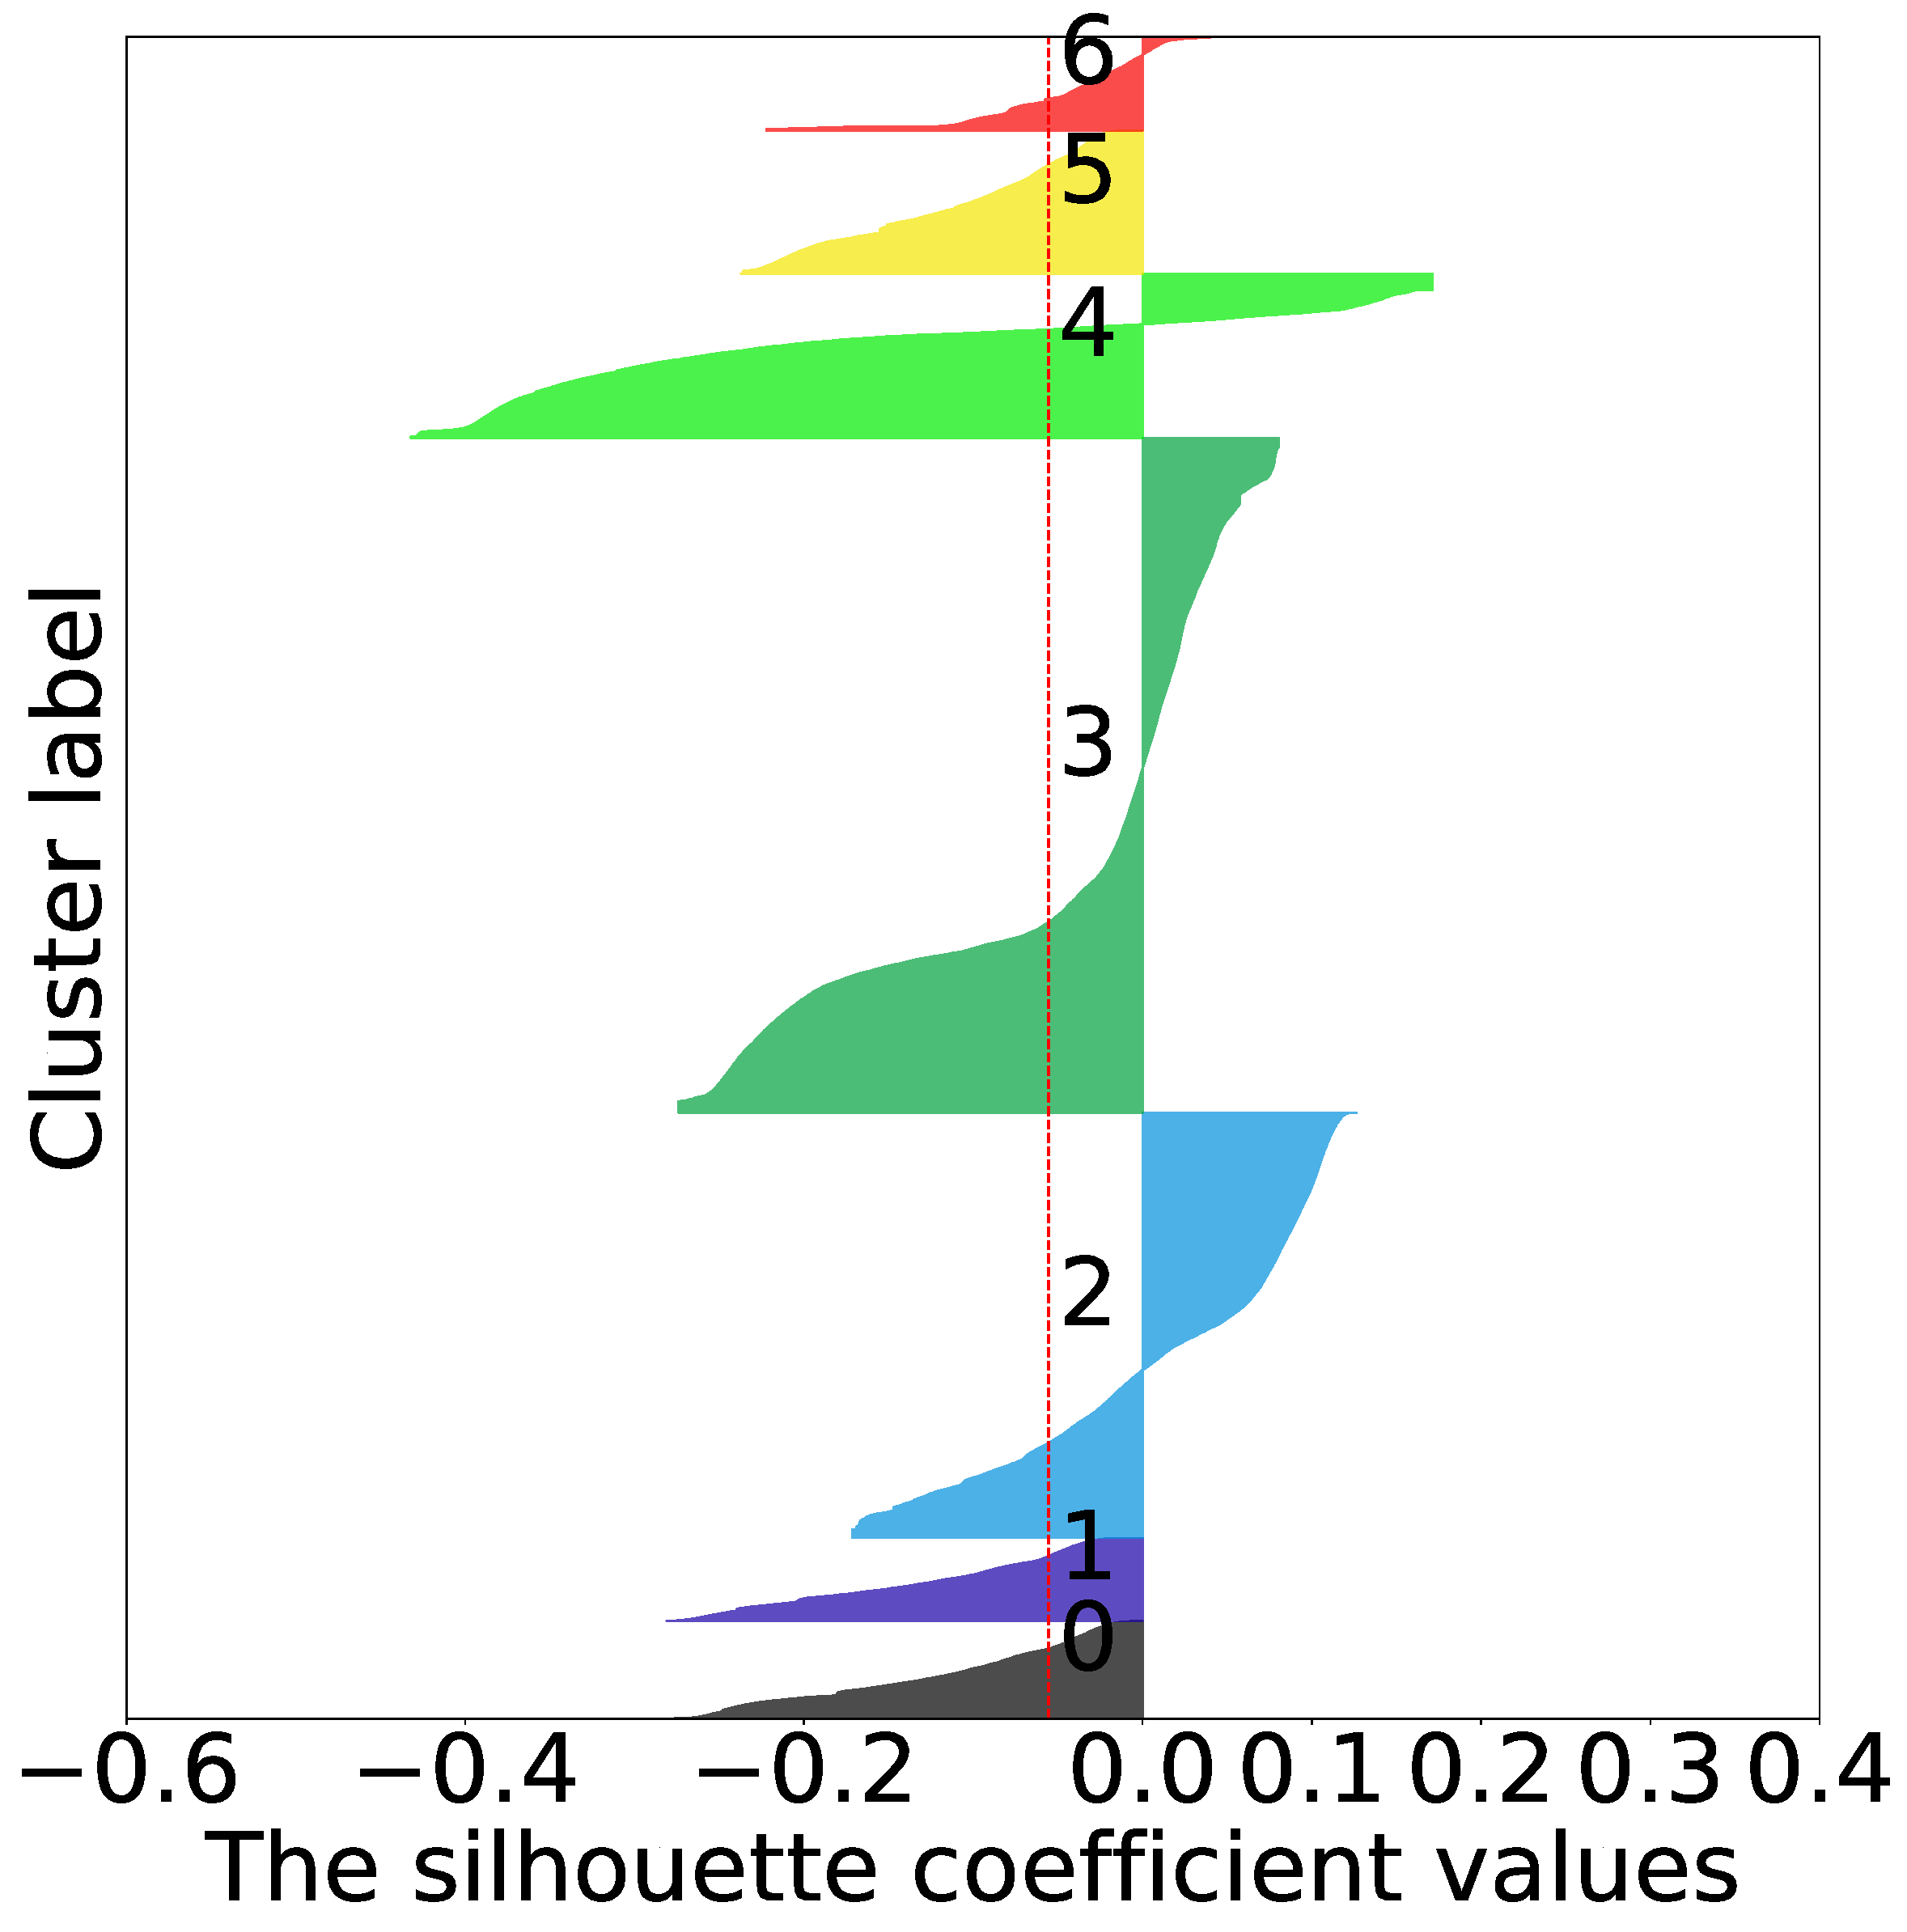
\includegraphics[width=0.45\textwidth]{figures/silhouette/silhouette_directly_7.pdf}
    }\\
    %     \subfloat[n\_clusters = 8]{
    %     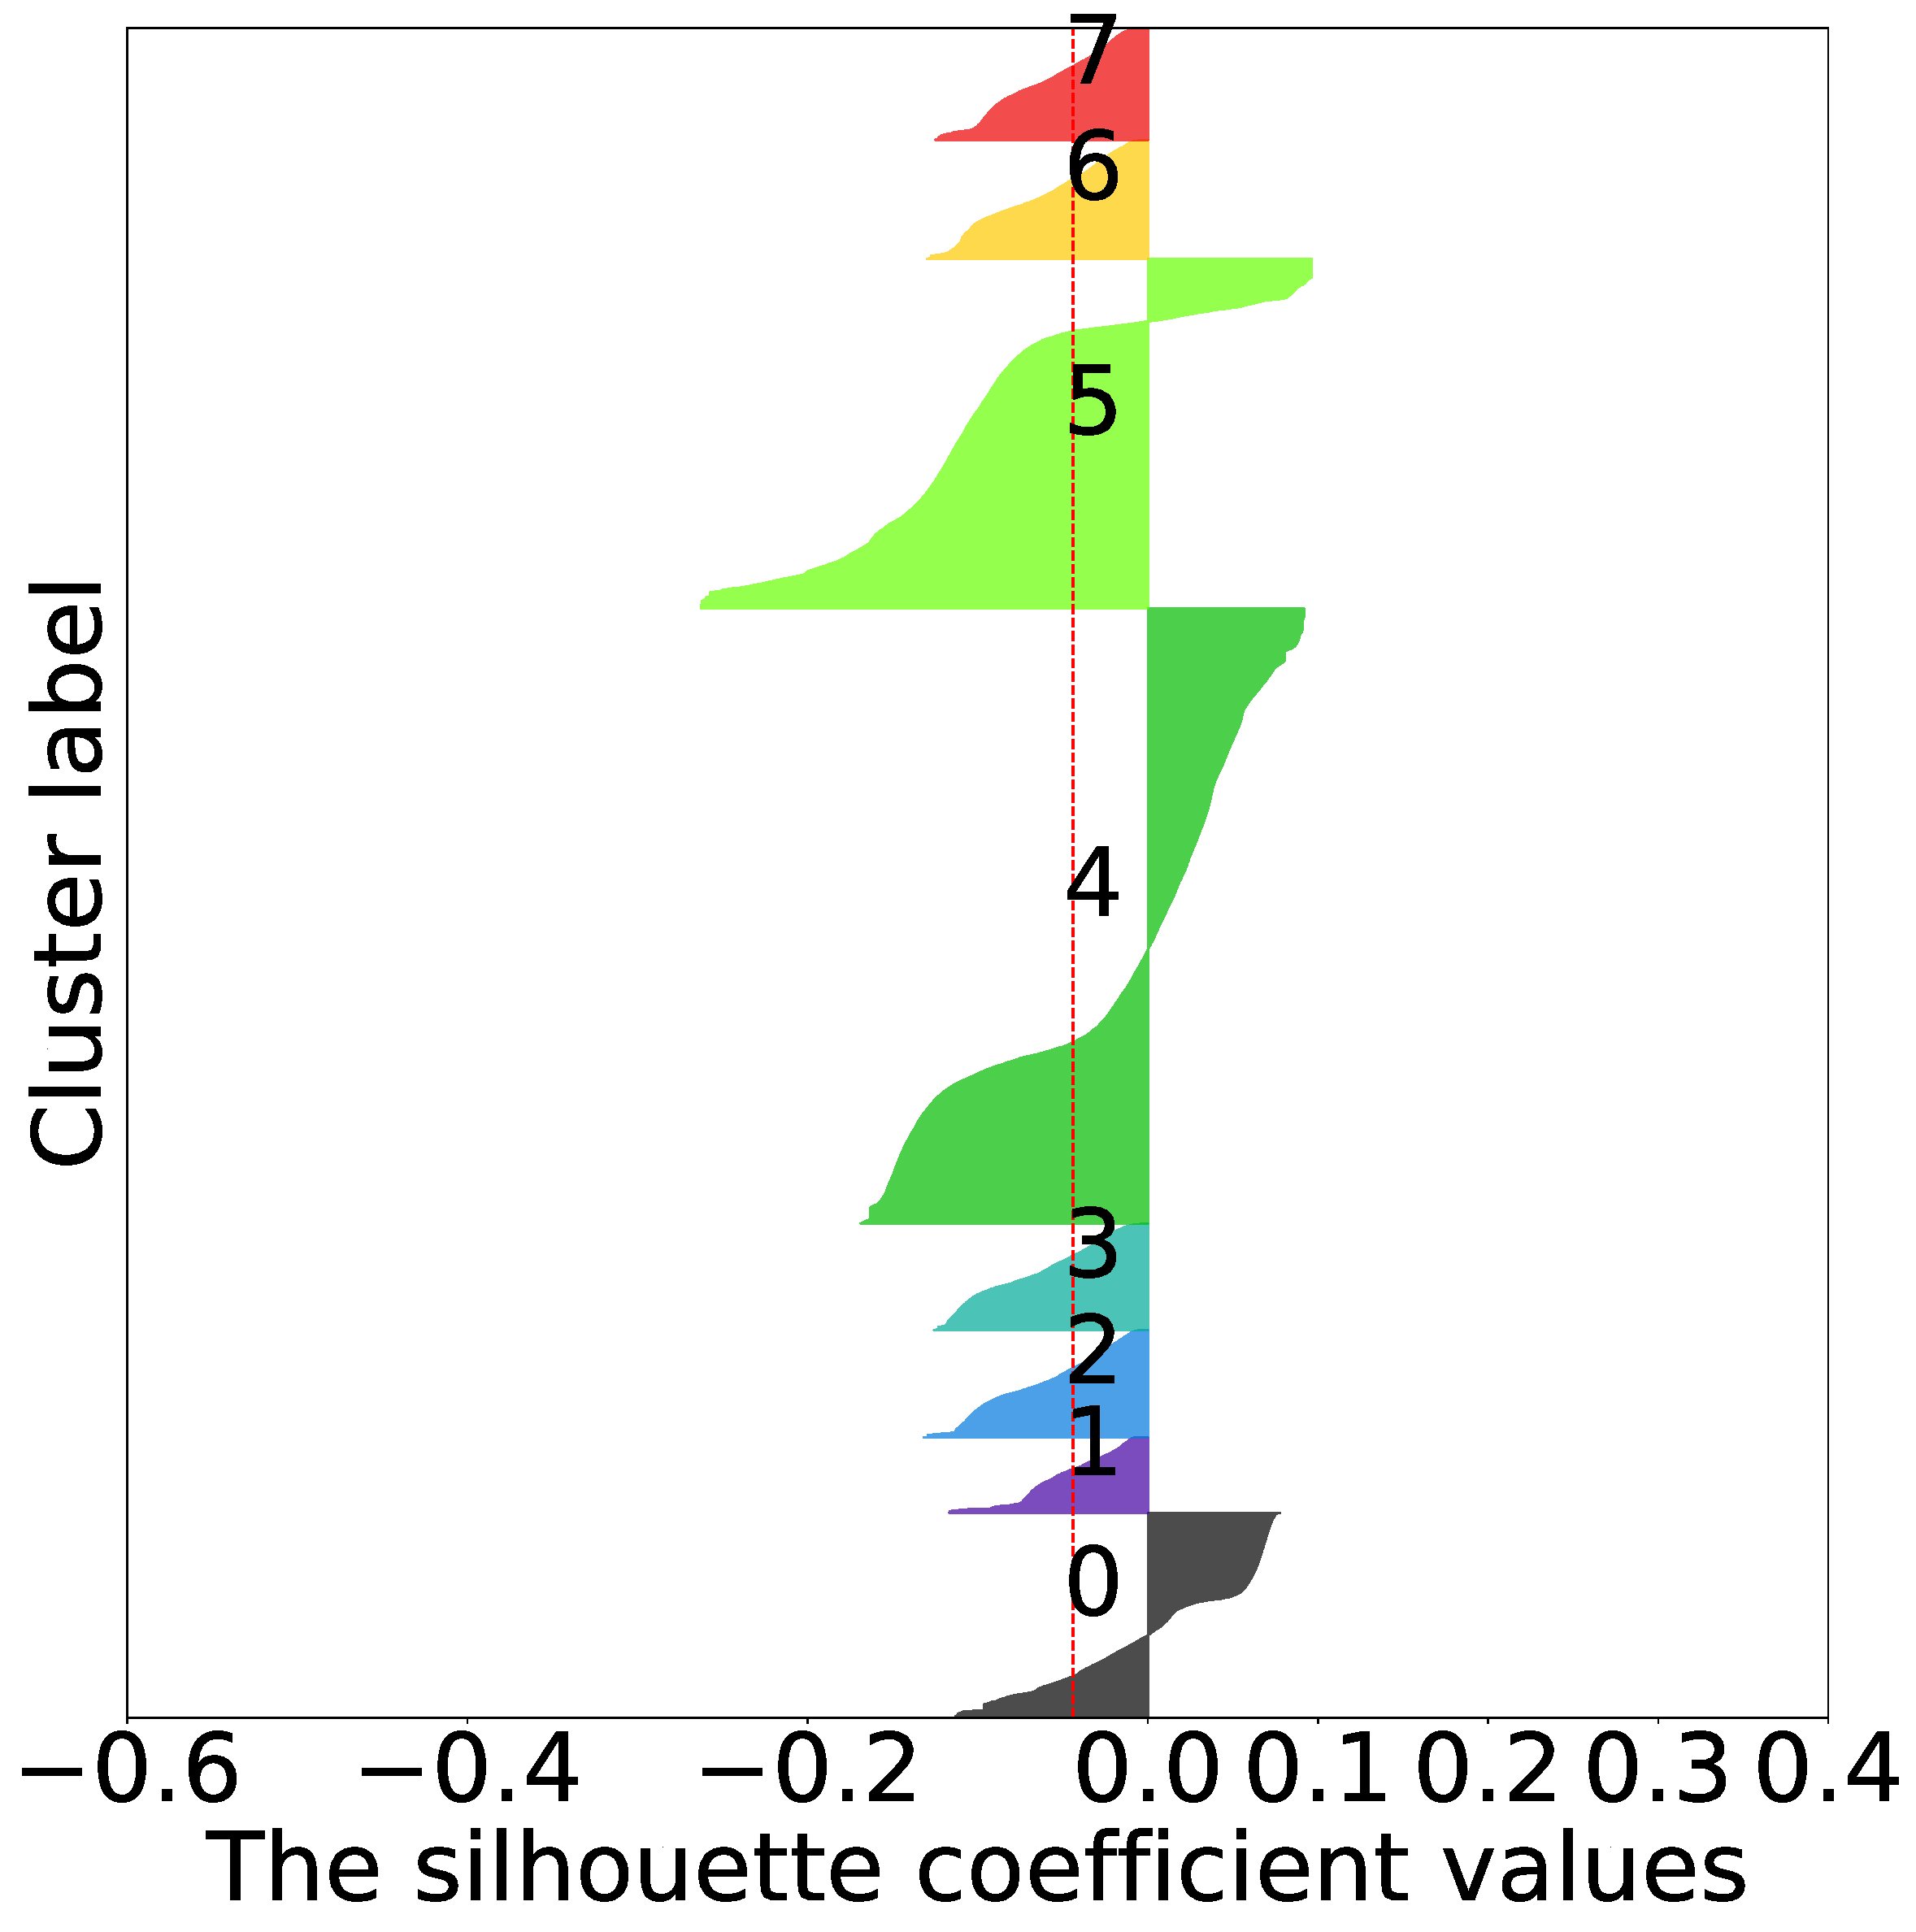
\includegraphics[width=0.5\textwidth]{figures/silhouette/silhouette_directly_8.pdf}
    % }
    %     \subfloat[n\_clusters = 9]{
    %     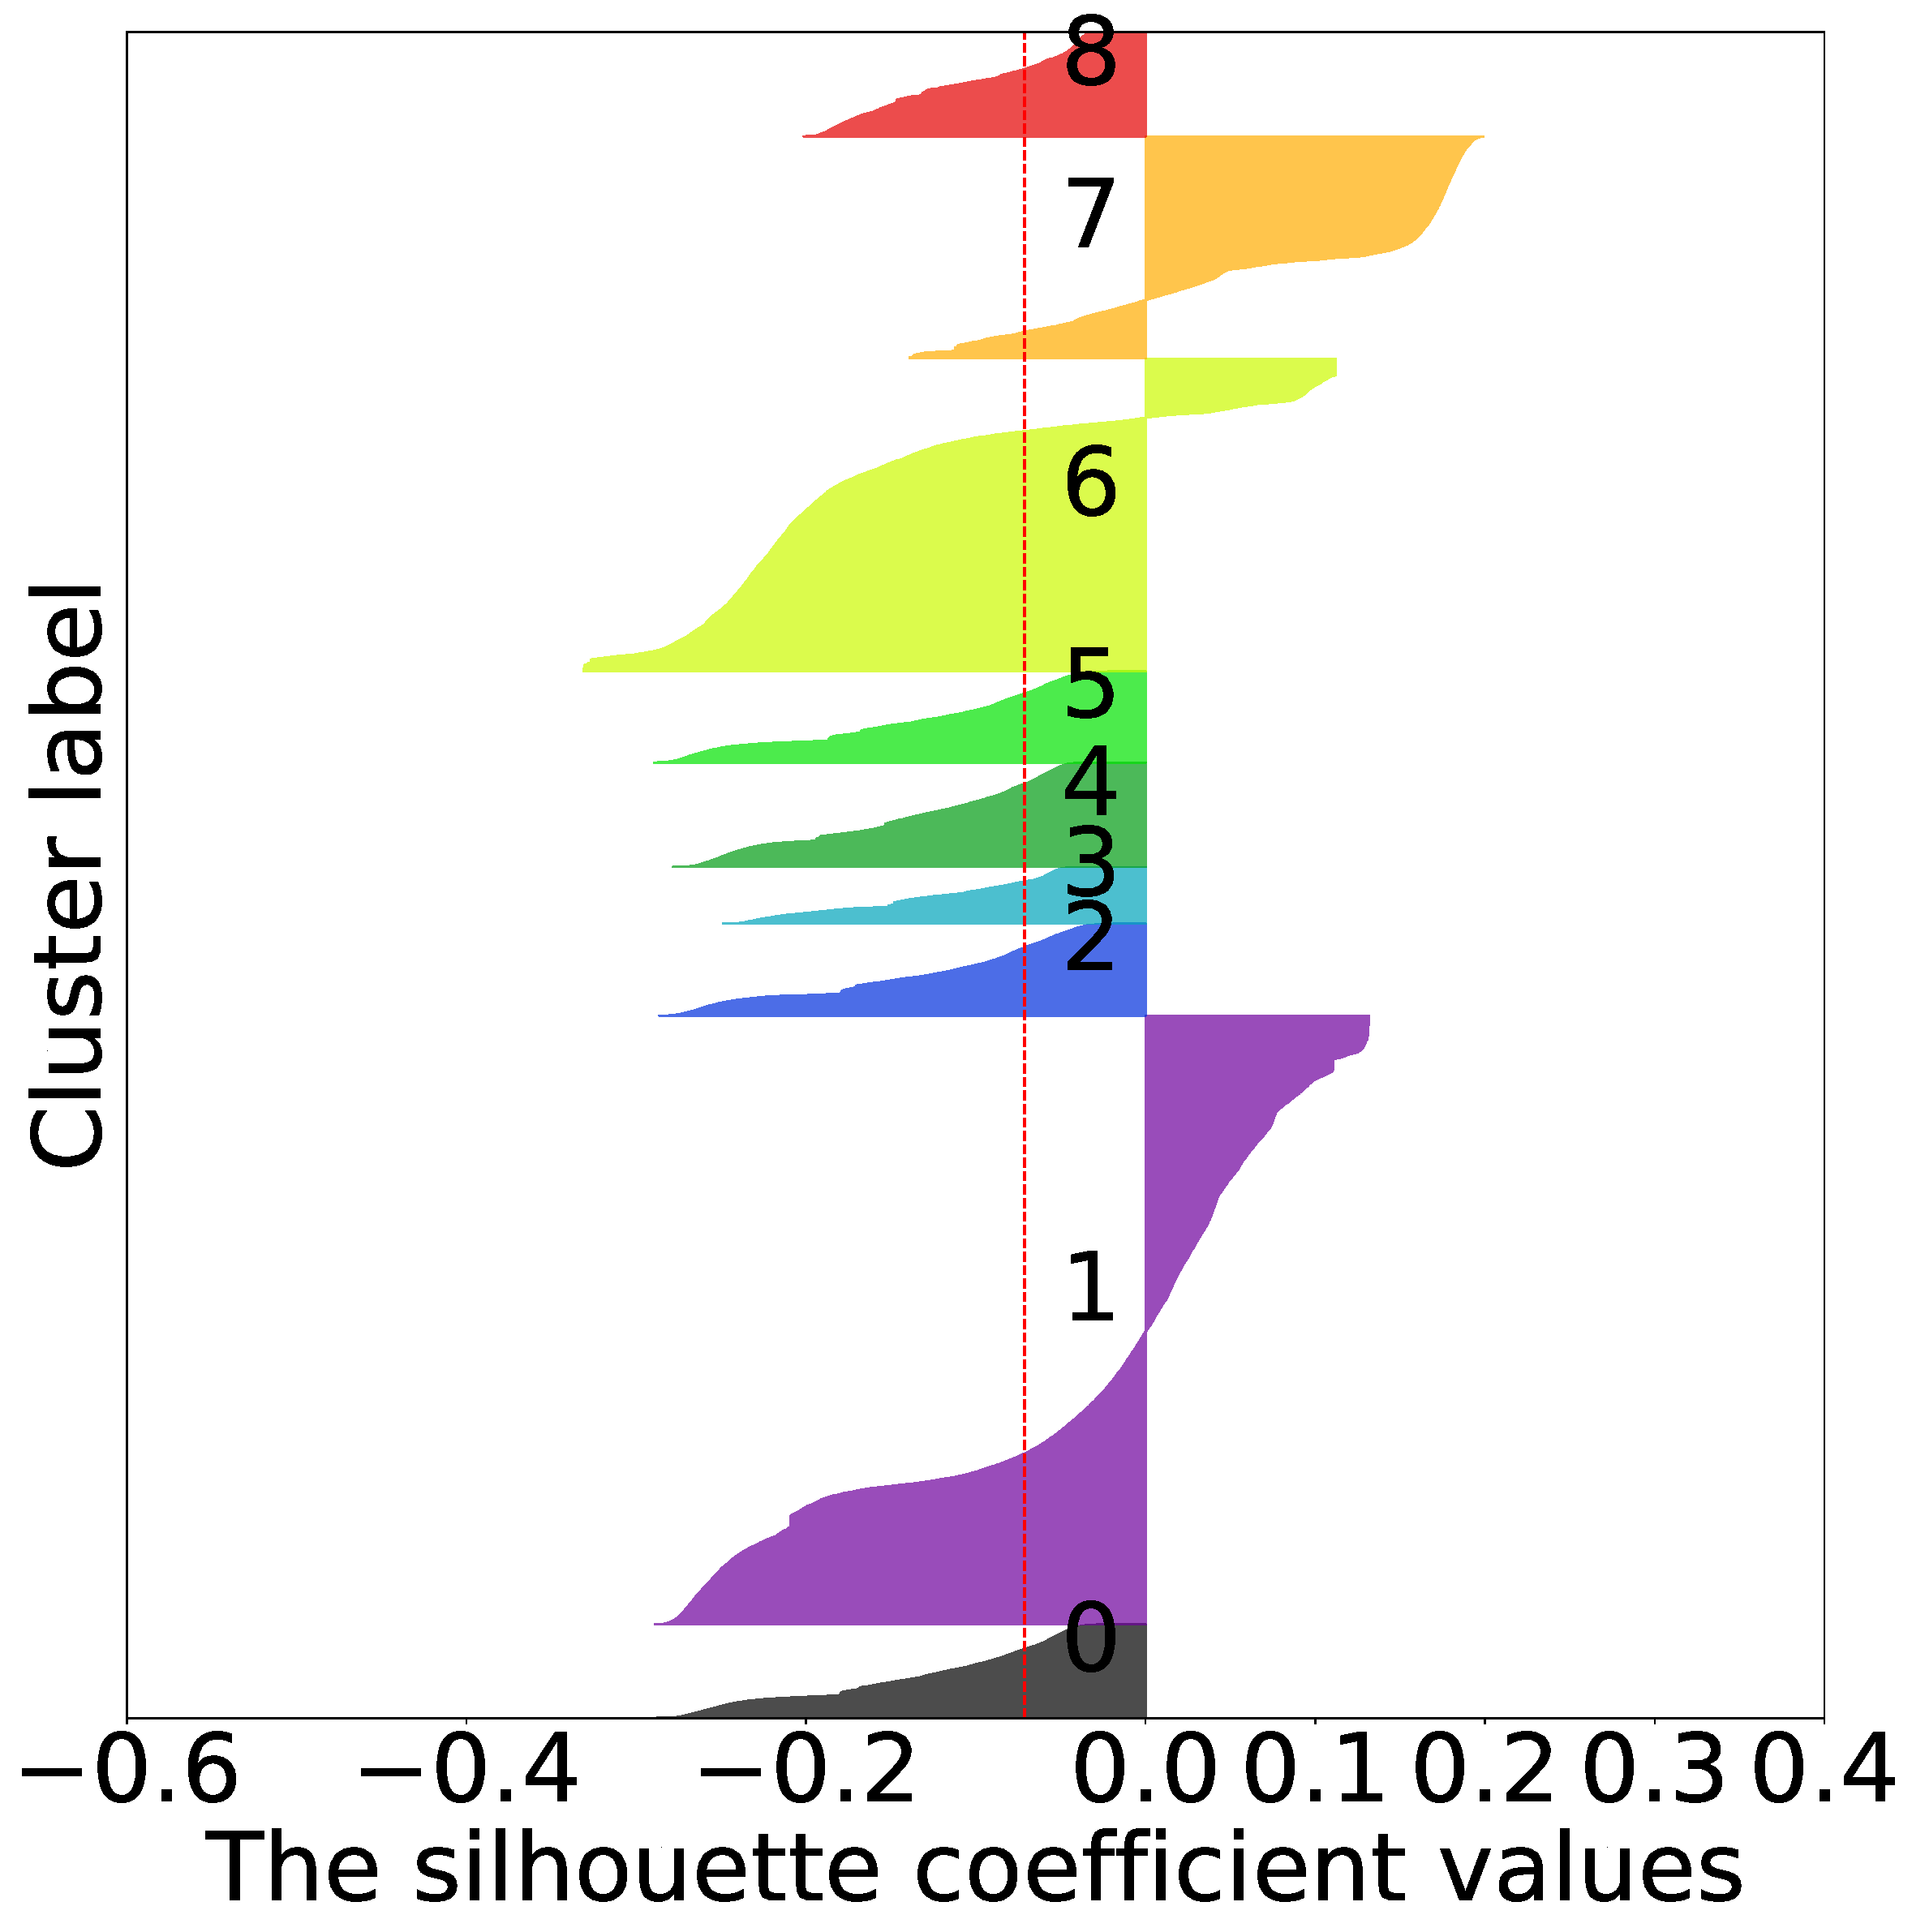
\includegraphics[width=0.5\textwidth]{figures/silhouette/silhouette_directly_9.pdf}
    % }\\
    %     \subfloat[n\_clusters = 10]{
    %     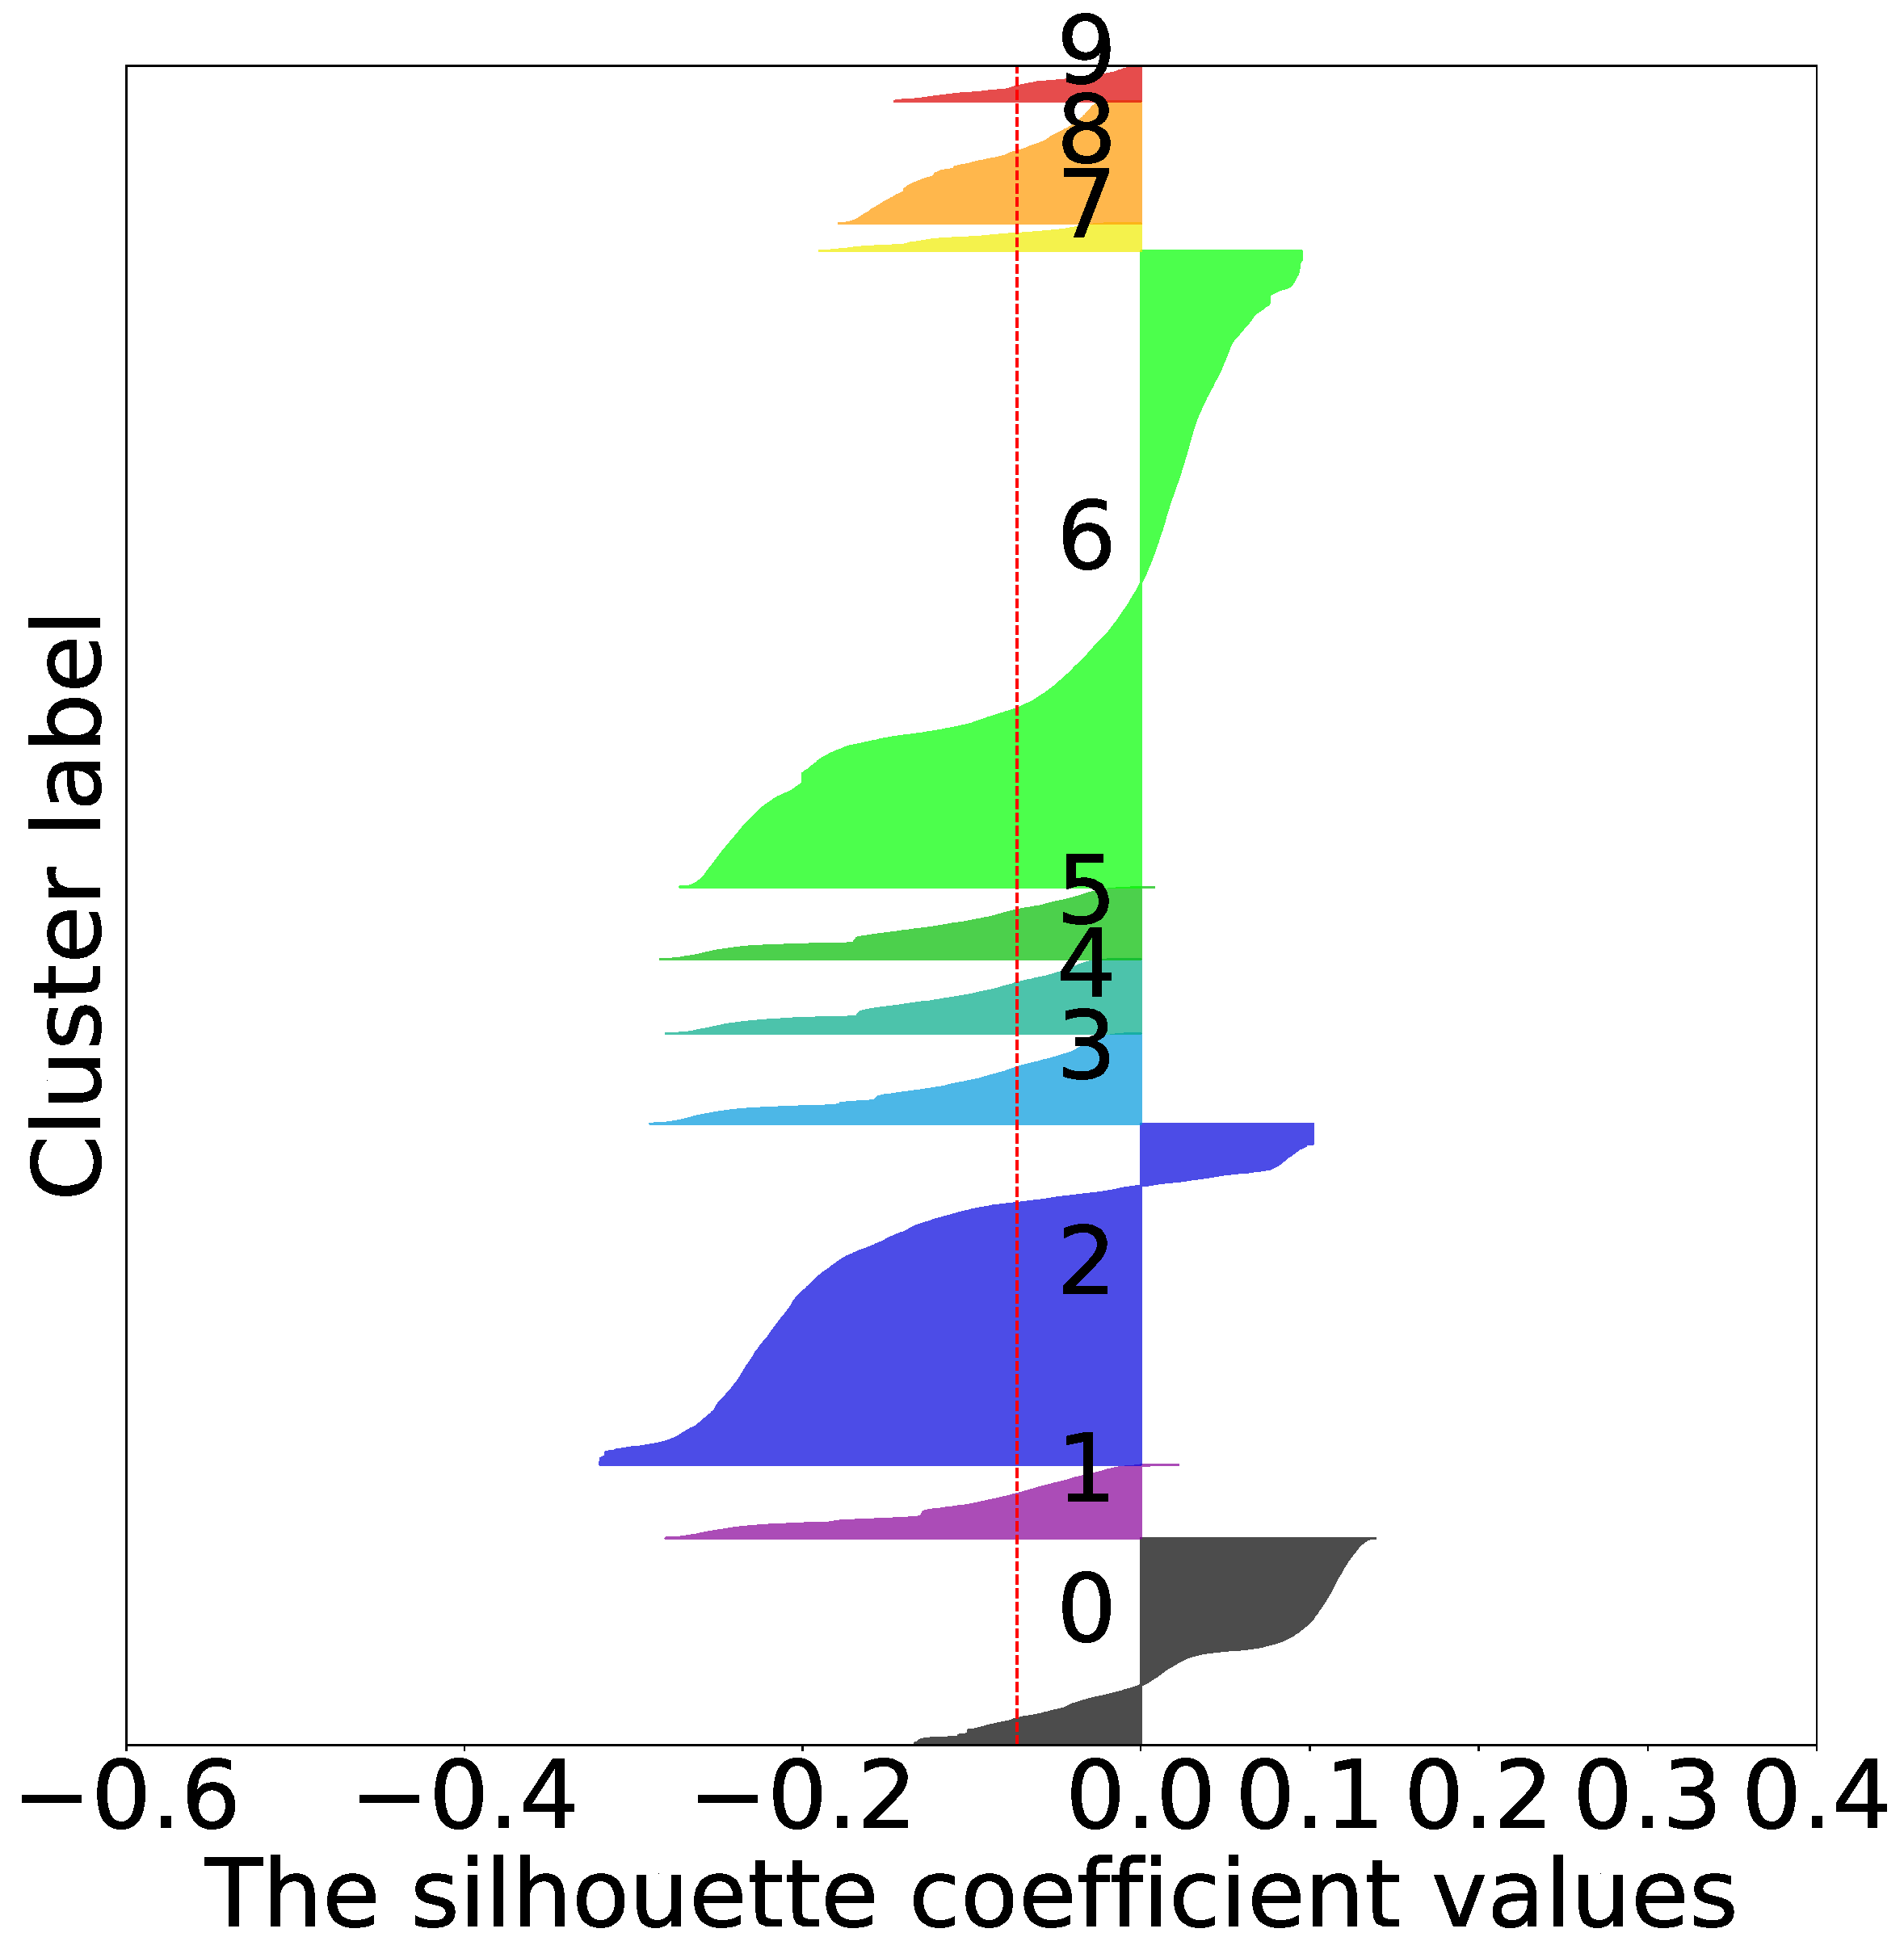
\includegraphics[width=0.5\textwidth]{figures/silhouette/silhouette_directly_10.pdf}
    % }
    \caption{Silhouette analysis of KMeans on raw windowed GPU load data}
    \label{fig_silhouette_directly}
\end{figure}

\begin{figure}[H]
    \centering
        \subfloat[n\_clusters = 2]{
        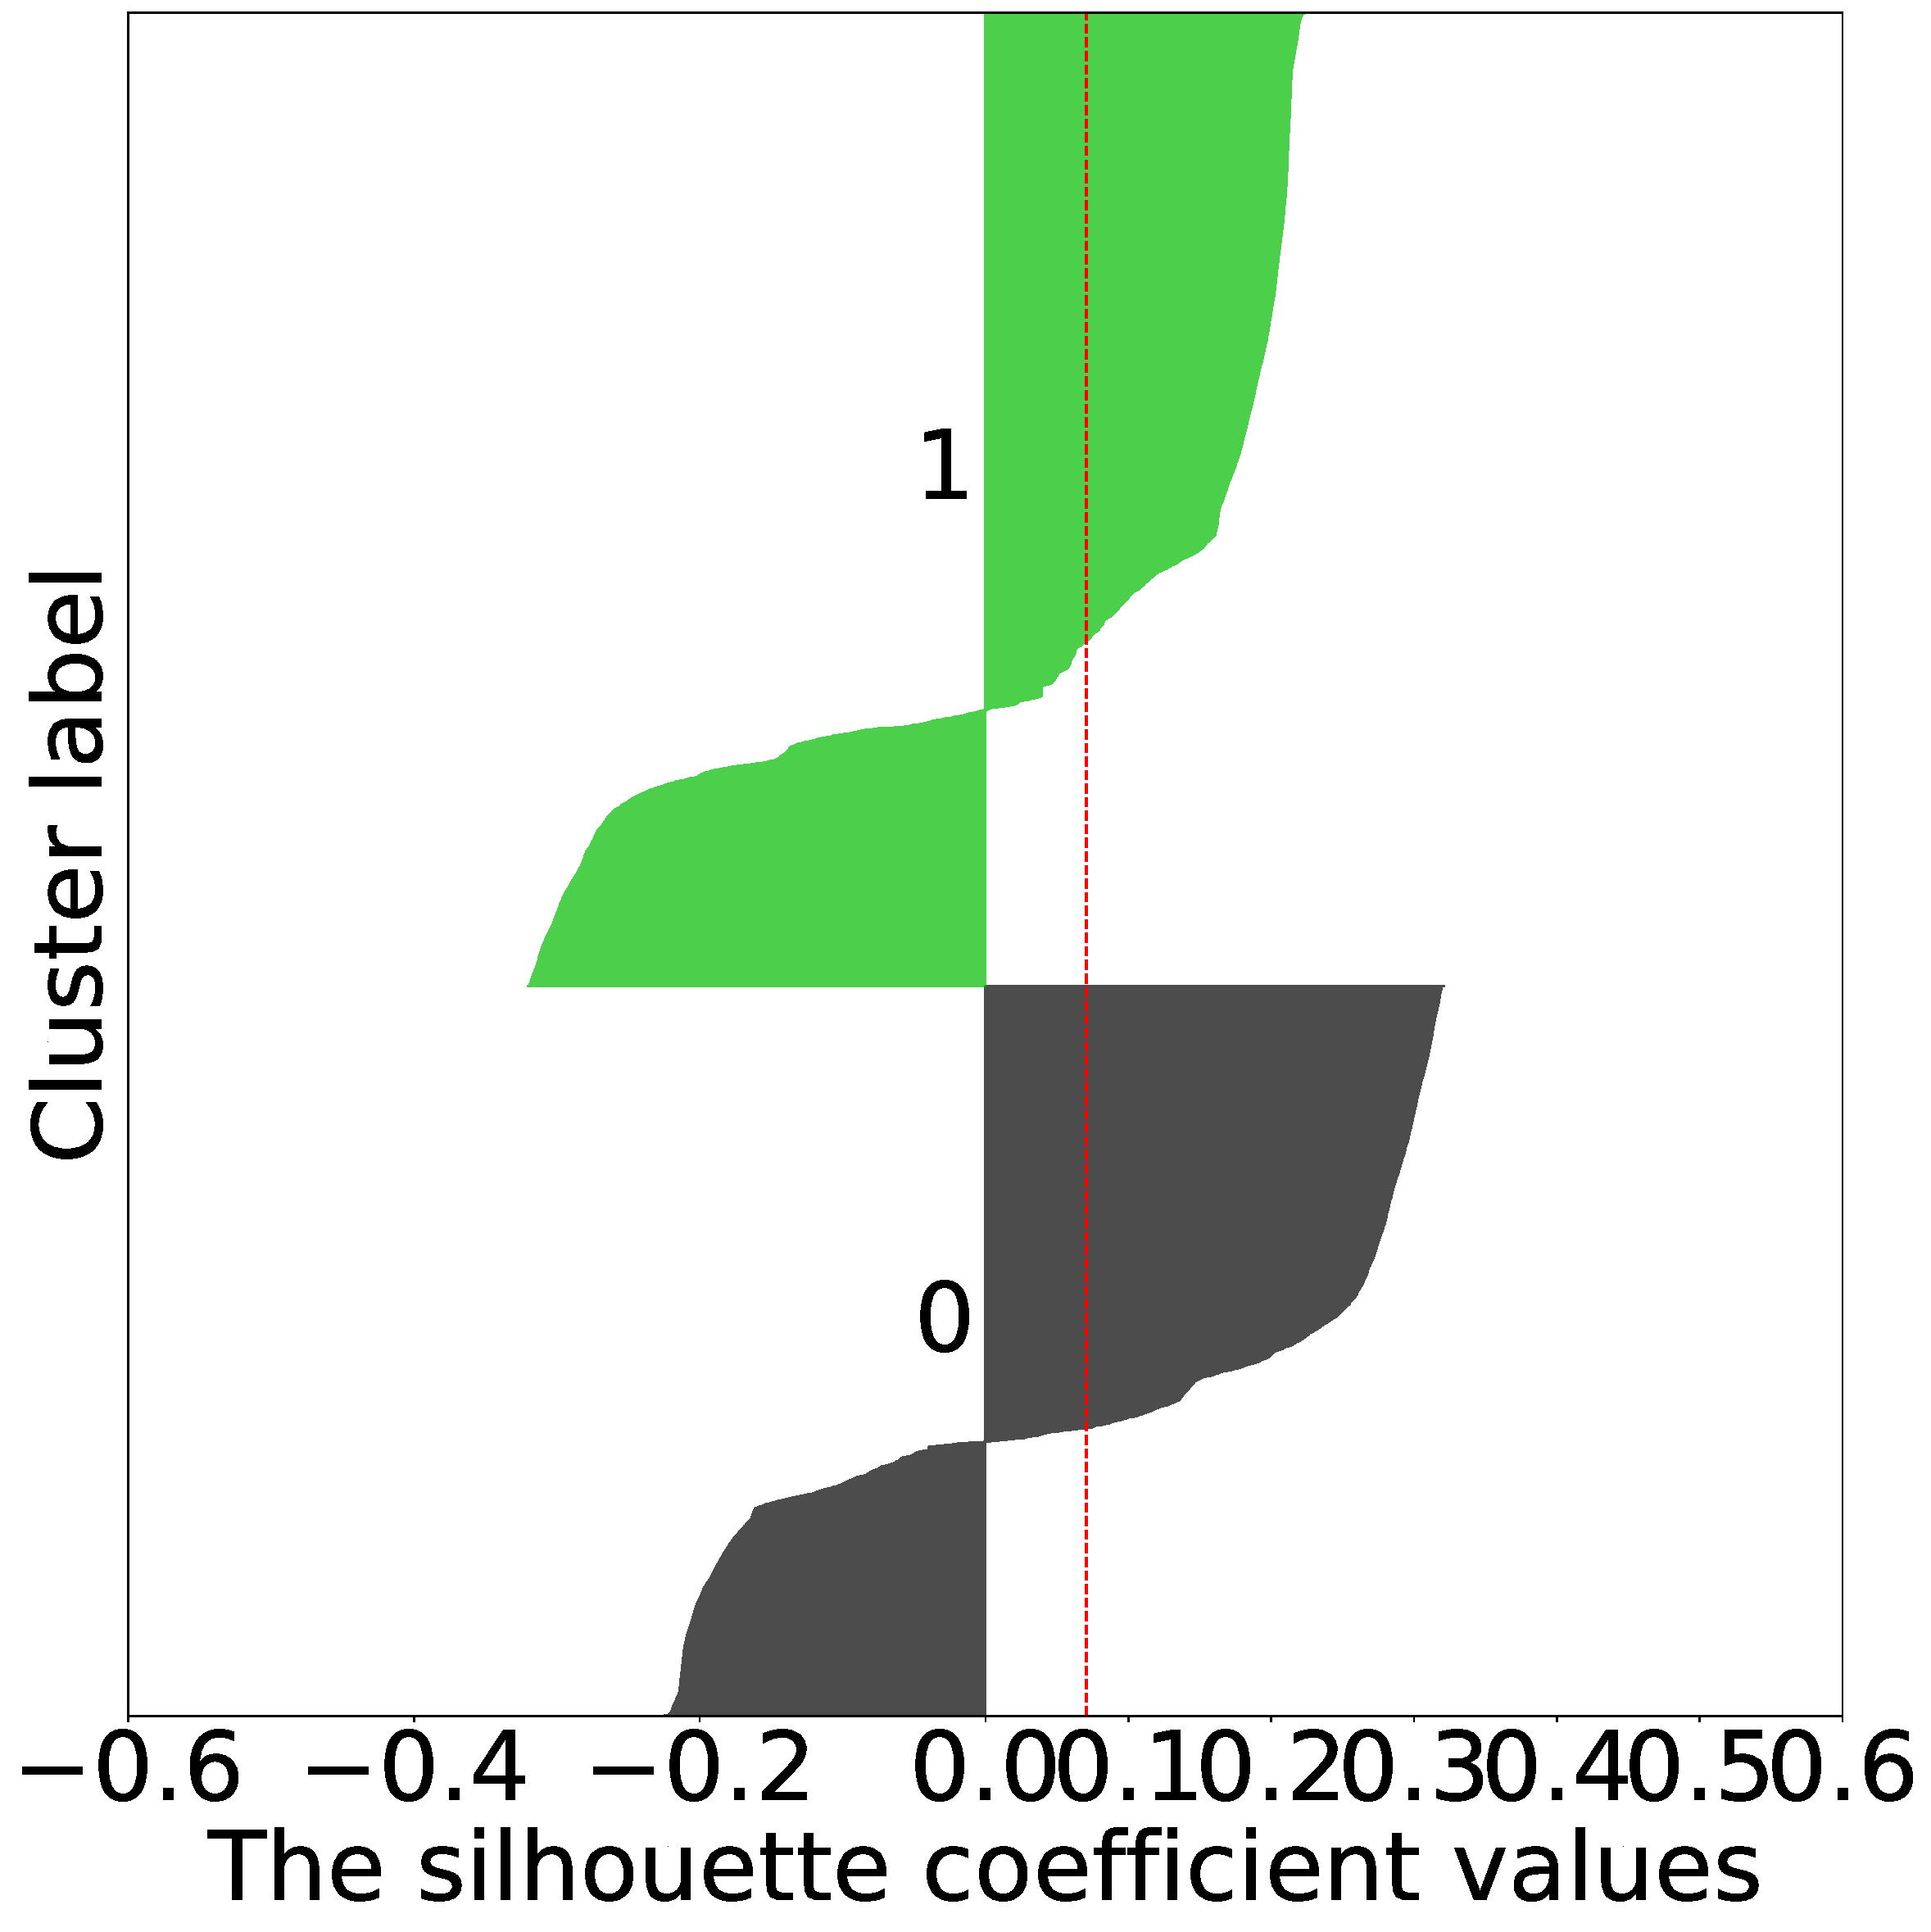
\includegraphics[width=0.45\textwidth]{figures/silhouette/silhouette_statistics_2.pdf}
    }
        \subfloat[n\_clusters = 3]{
        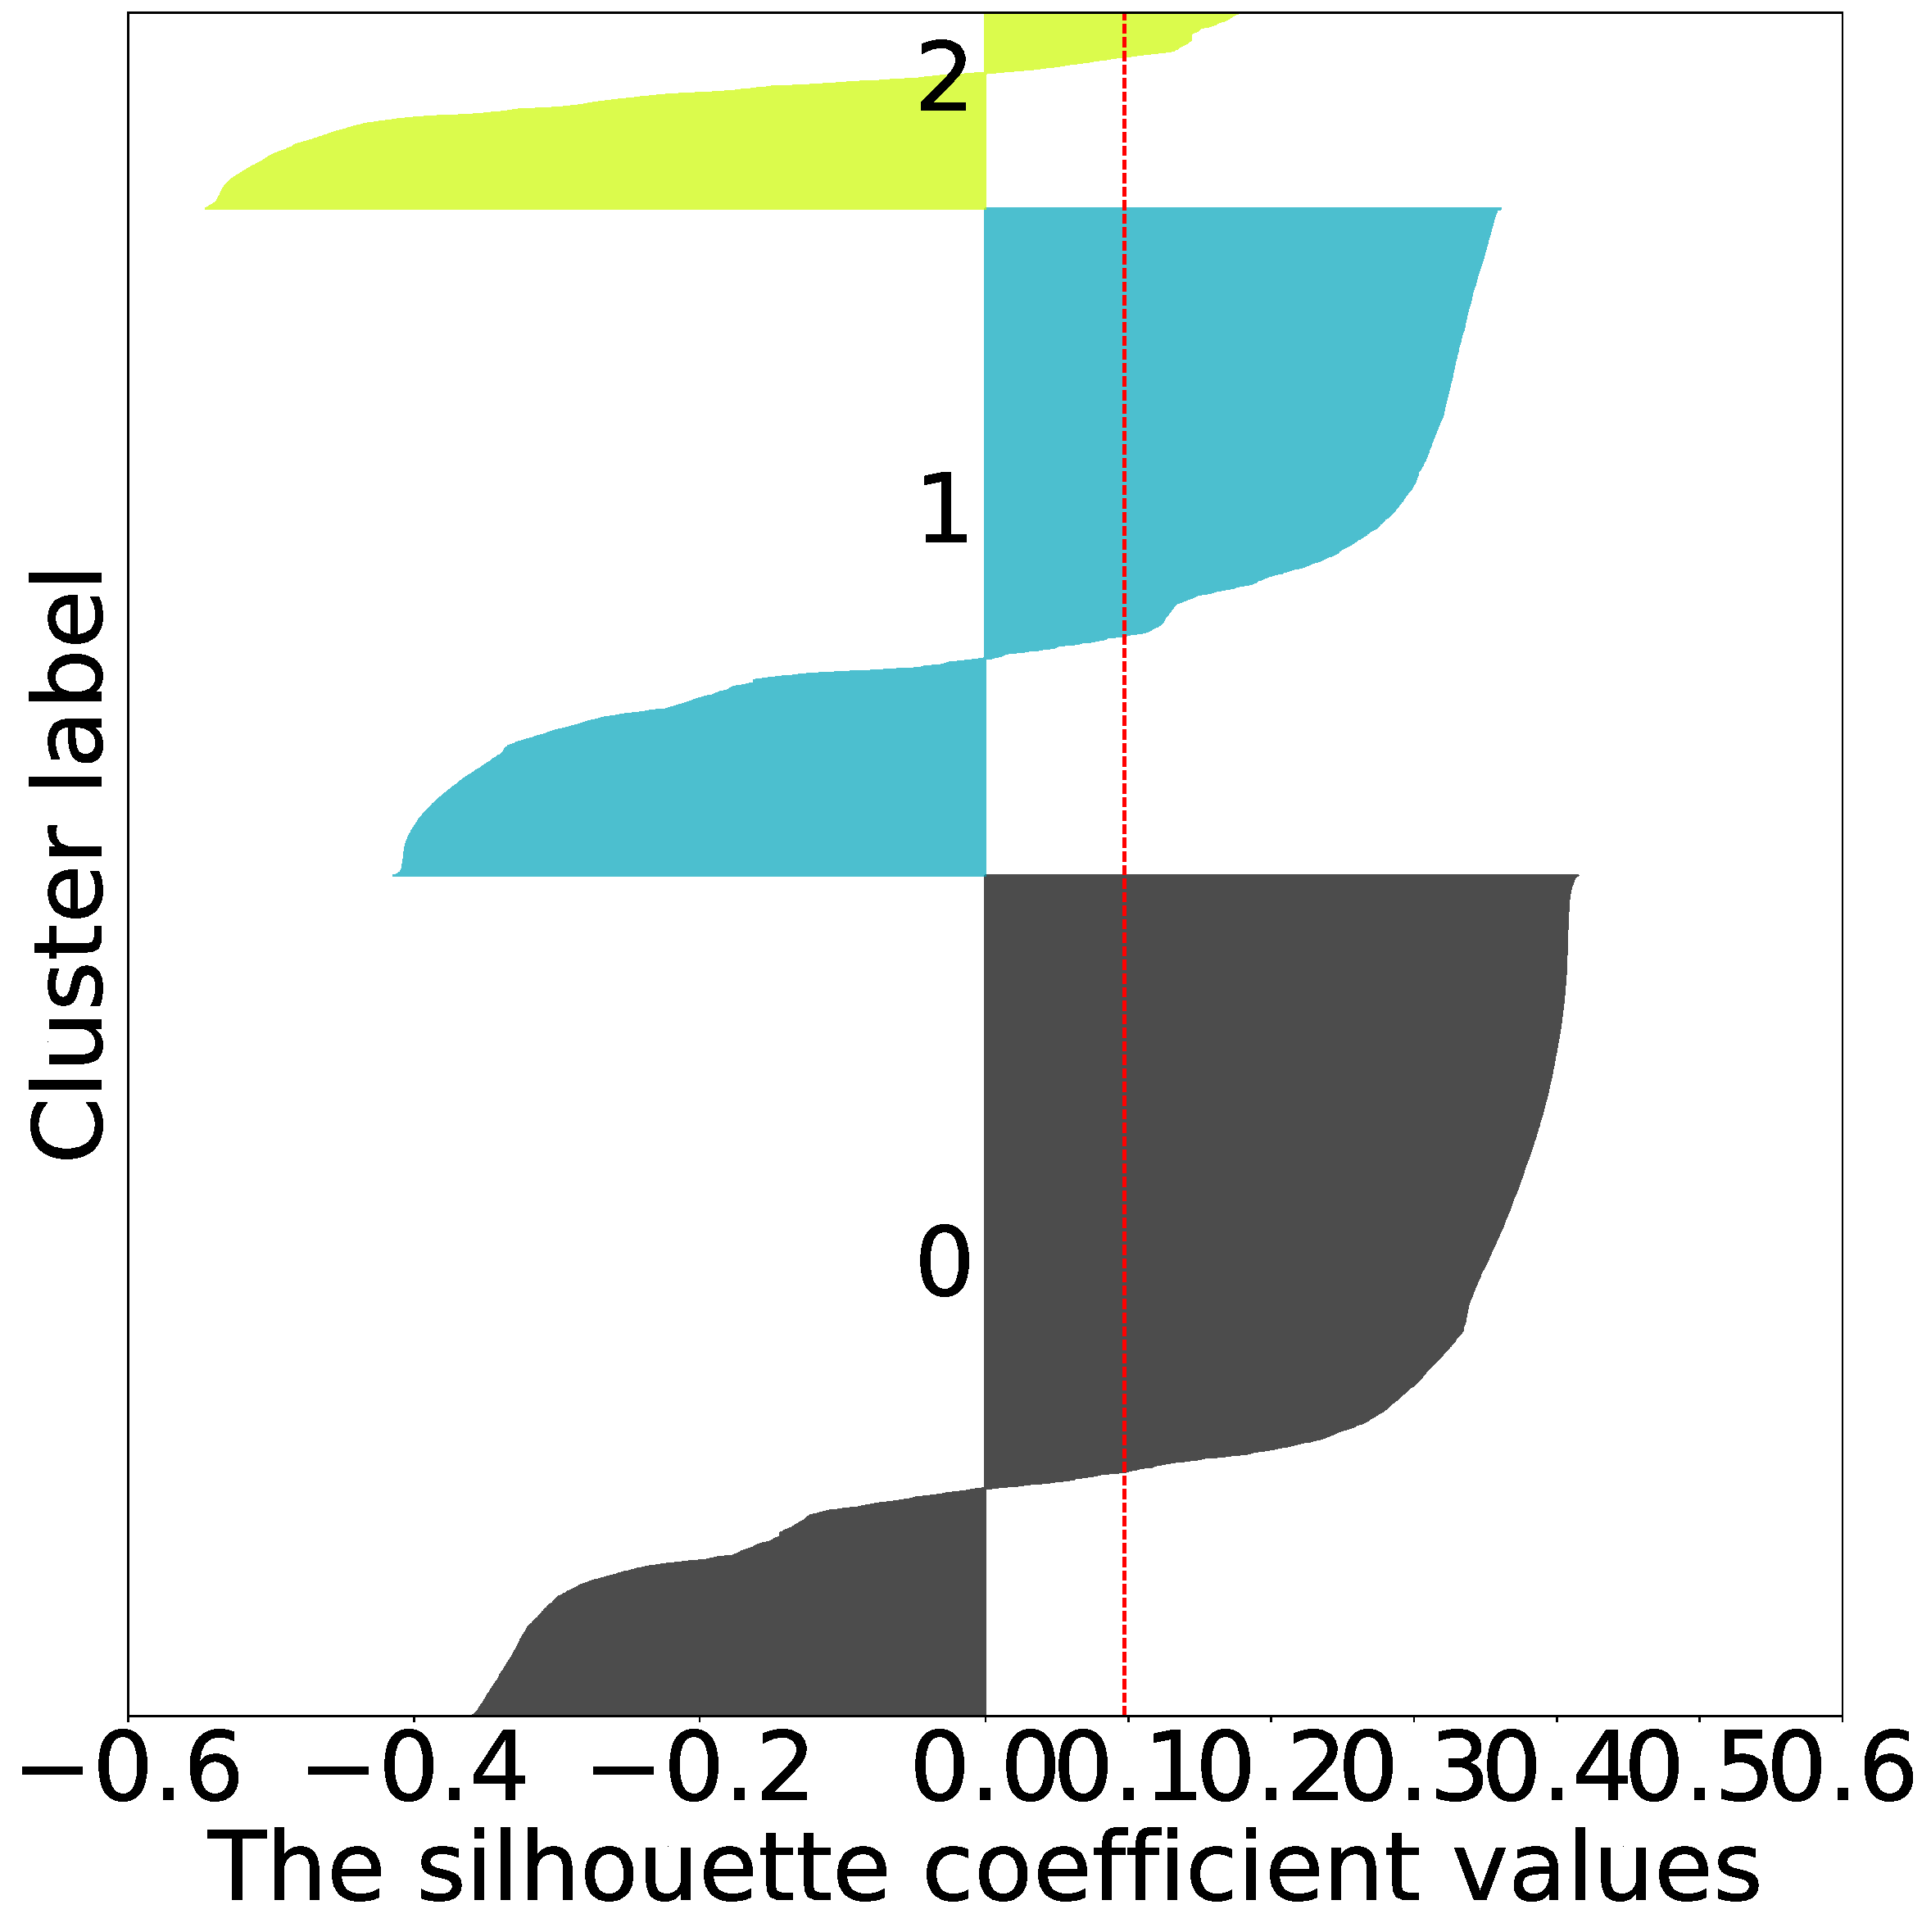
\includegraphics[width=0.45\textwidth]{figures/silhouette/silhouette_statistics_3.pdf}
    }\\
        \subfloat[n\_clusters = 4]{
        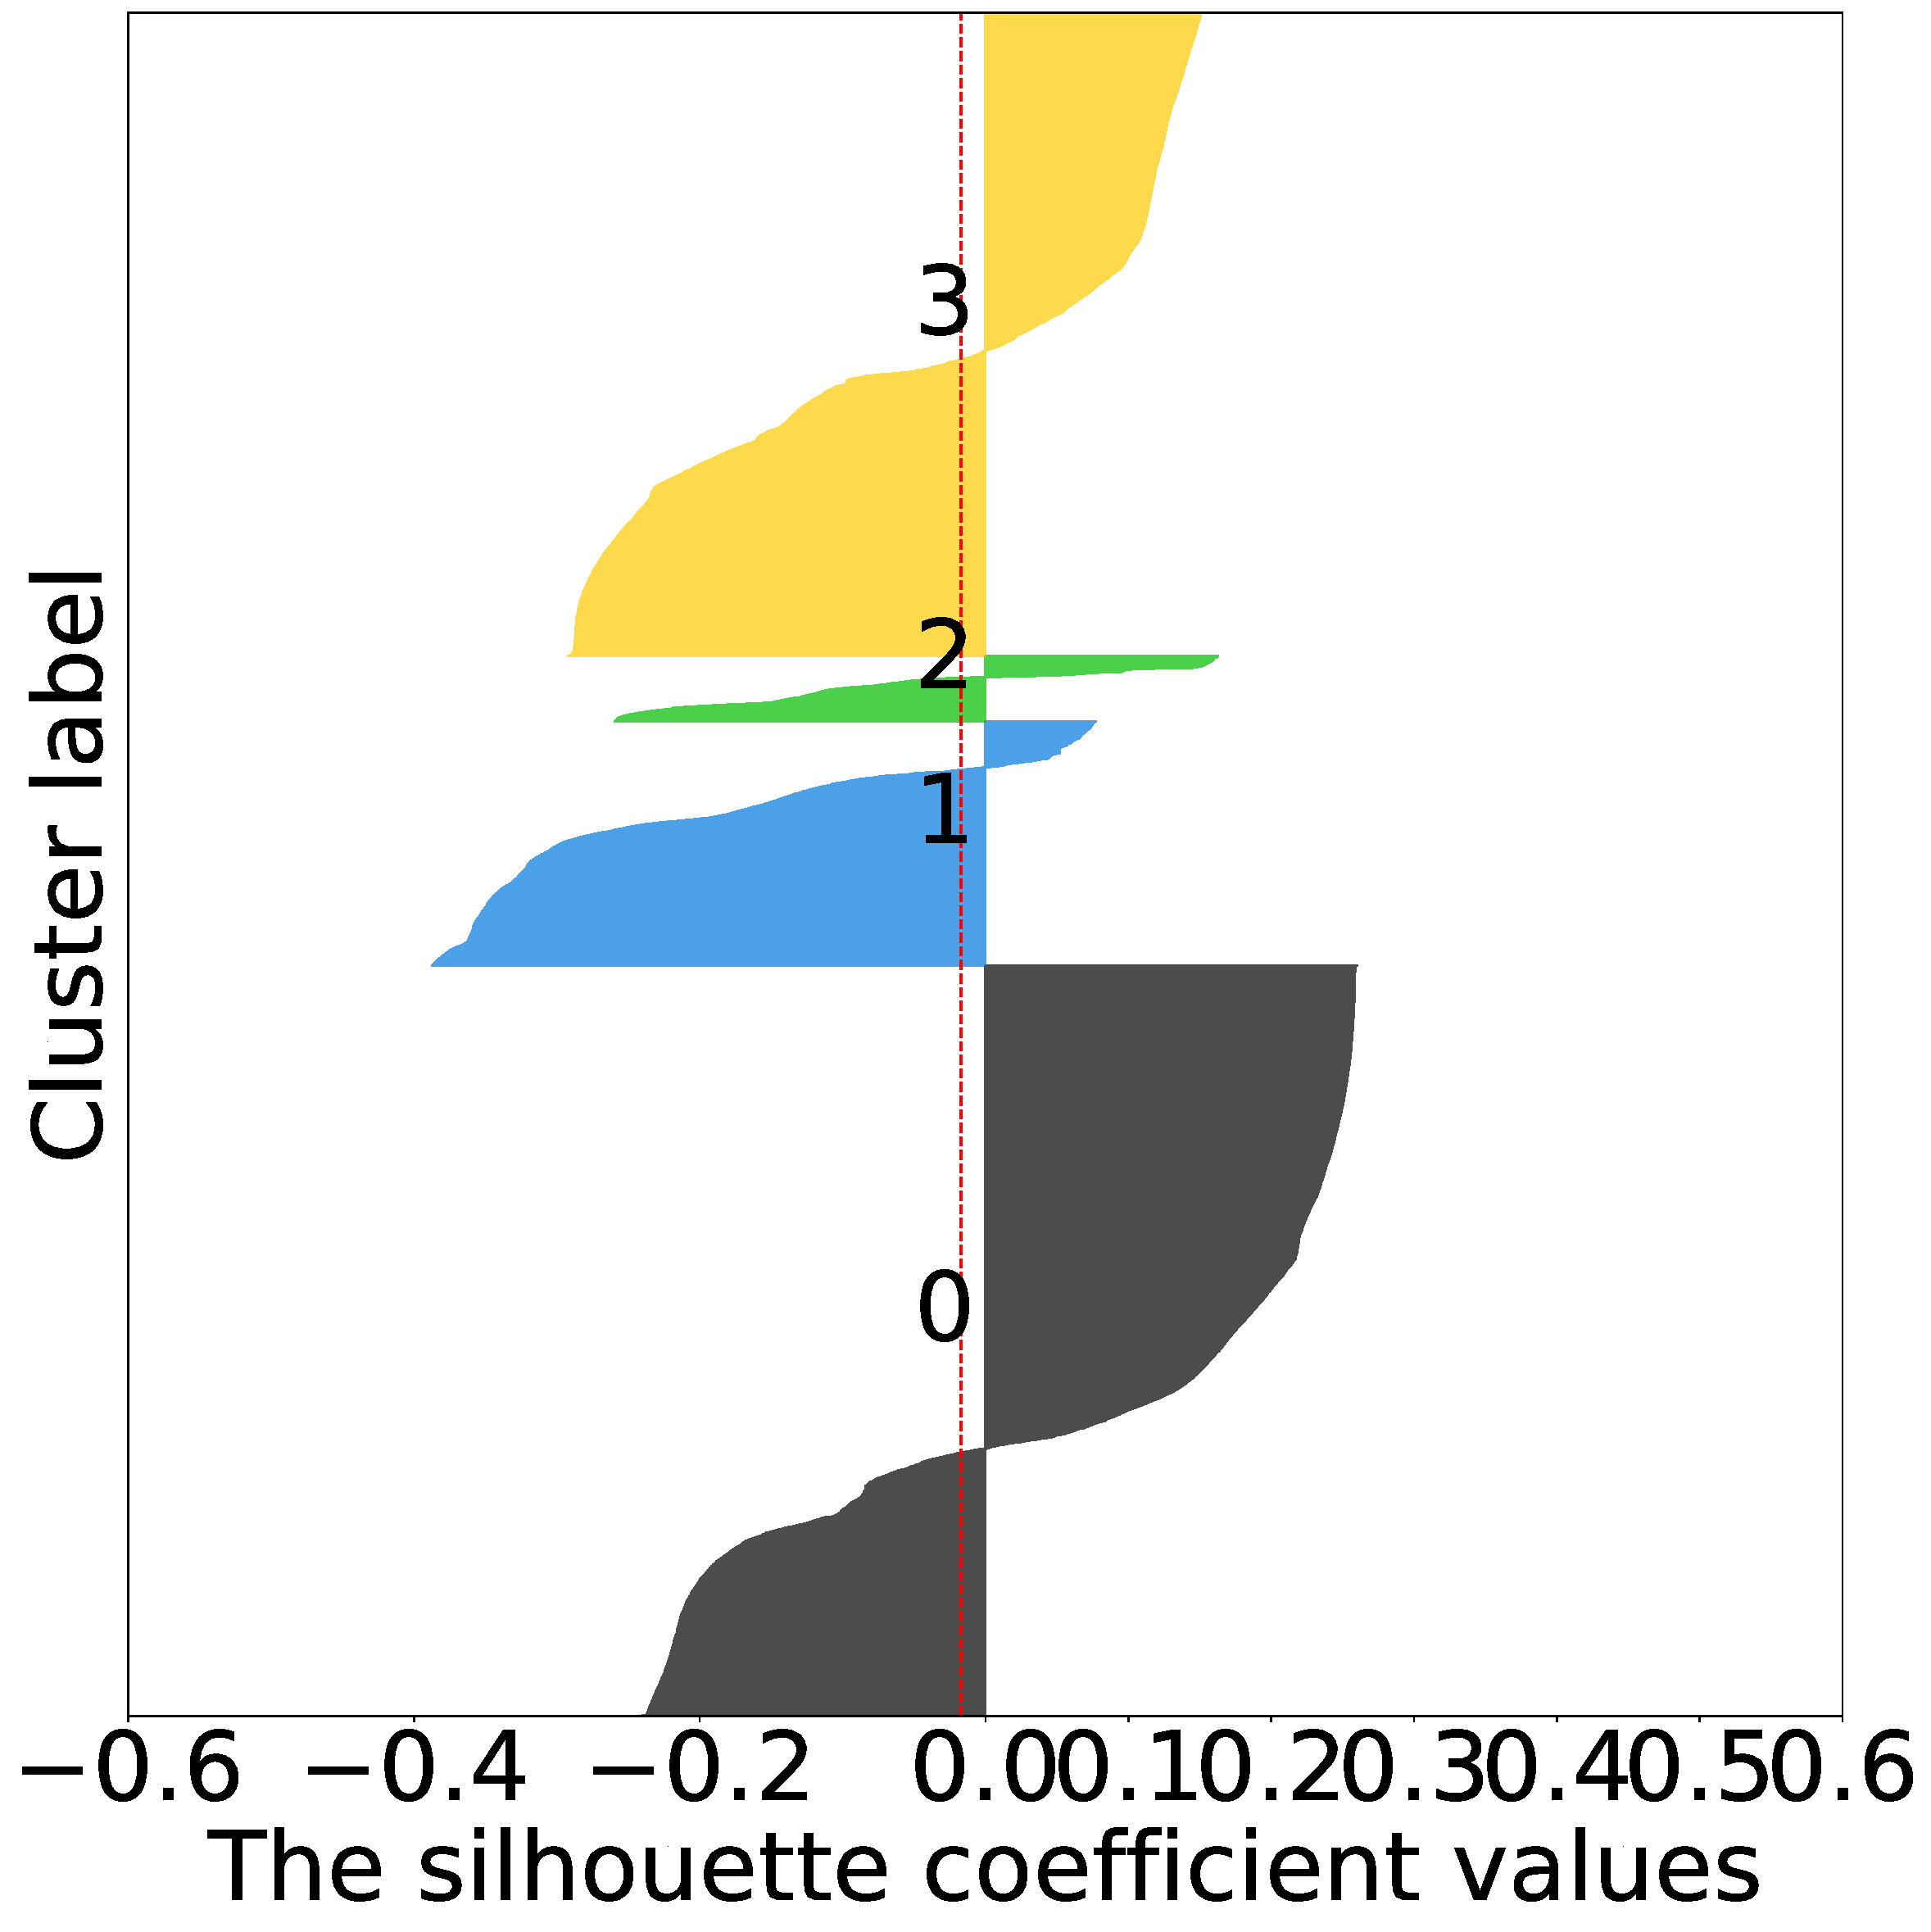
\includegraphics[width=0.45\textwidth]{figures/silhouette/silhouette_statistics_4.pdf}
    }
        \subfloat[n\_clusters = 5]{
        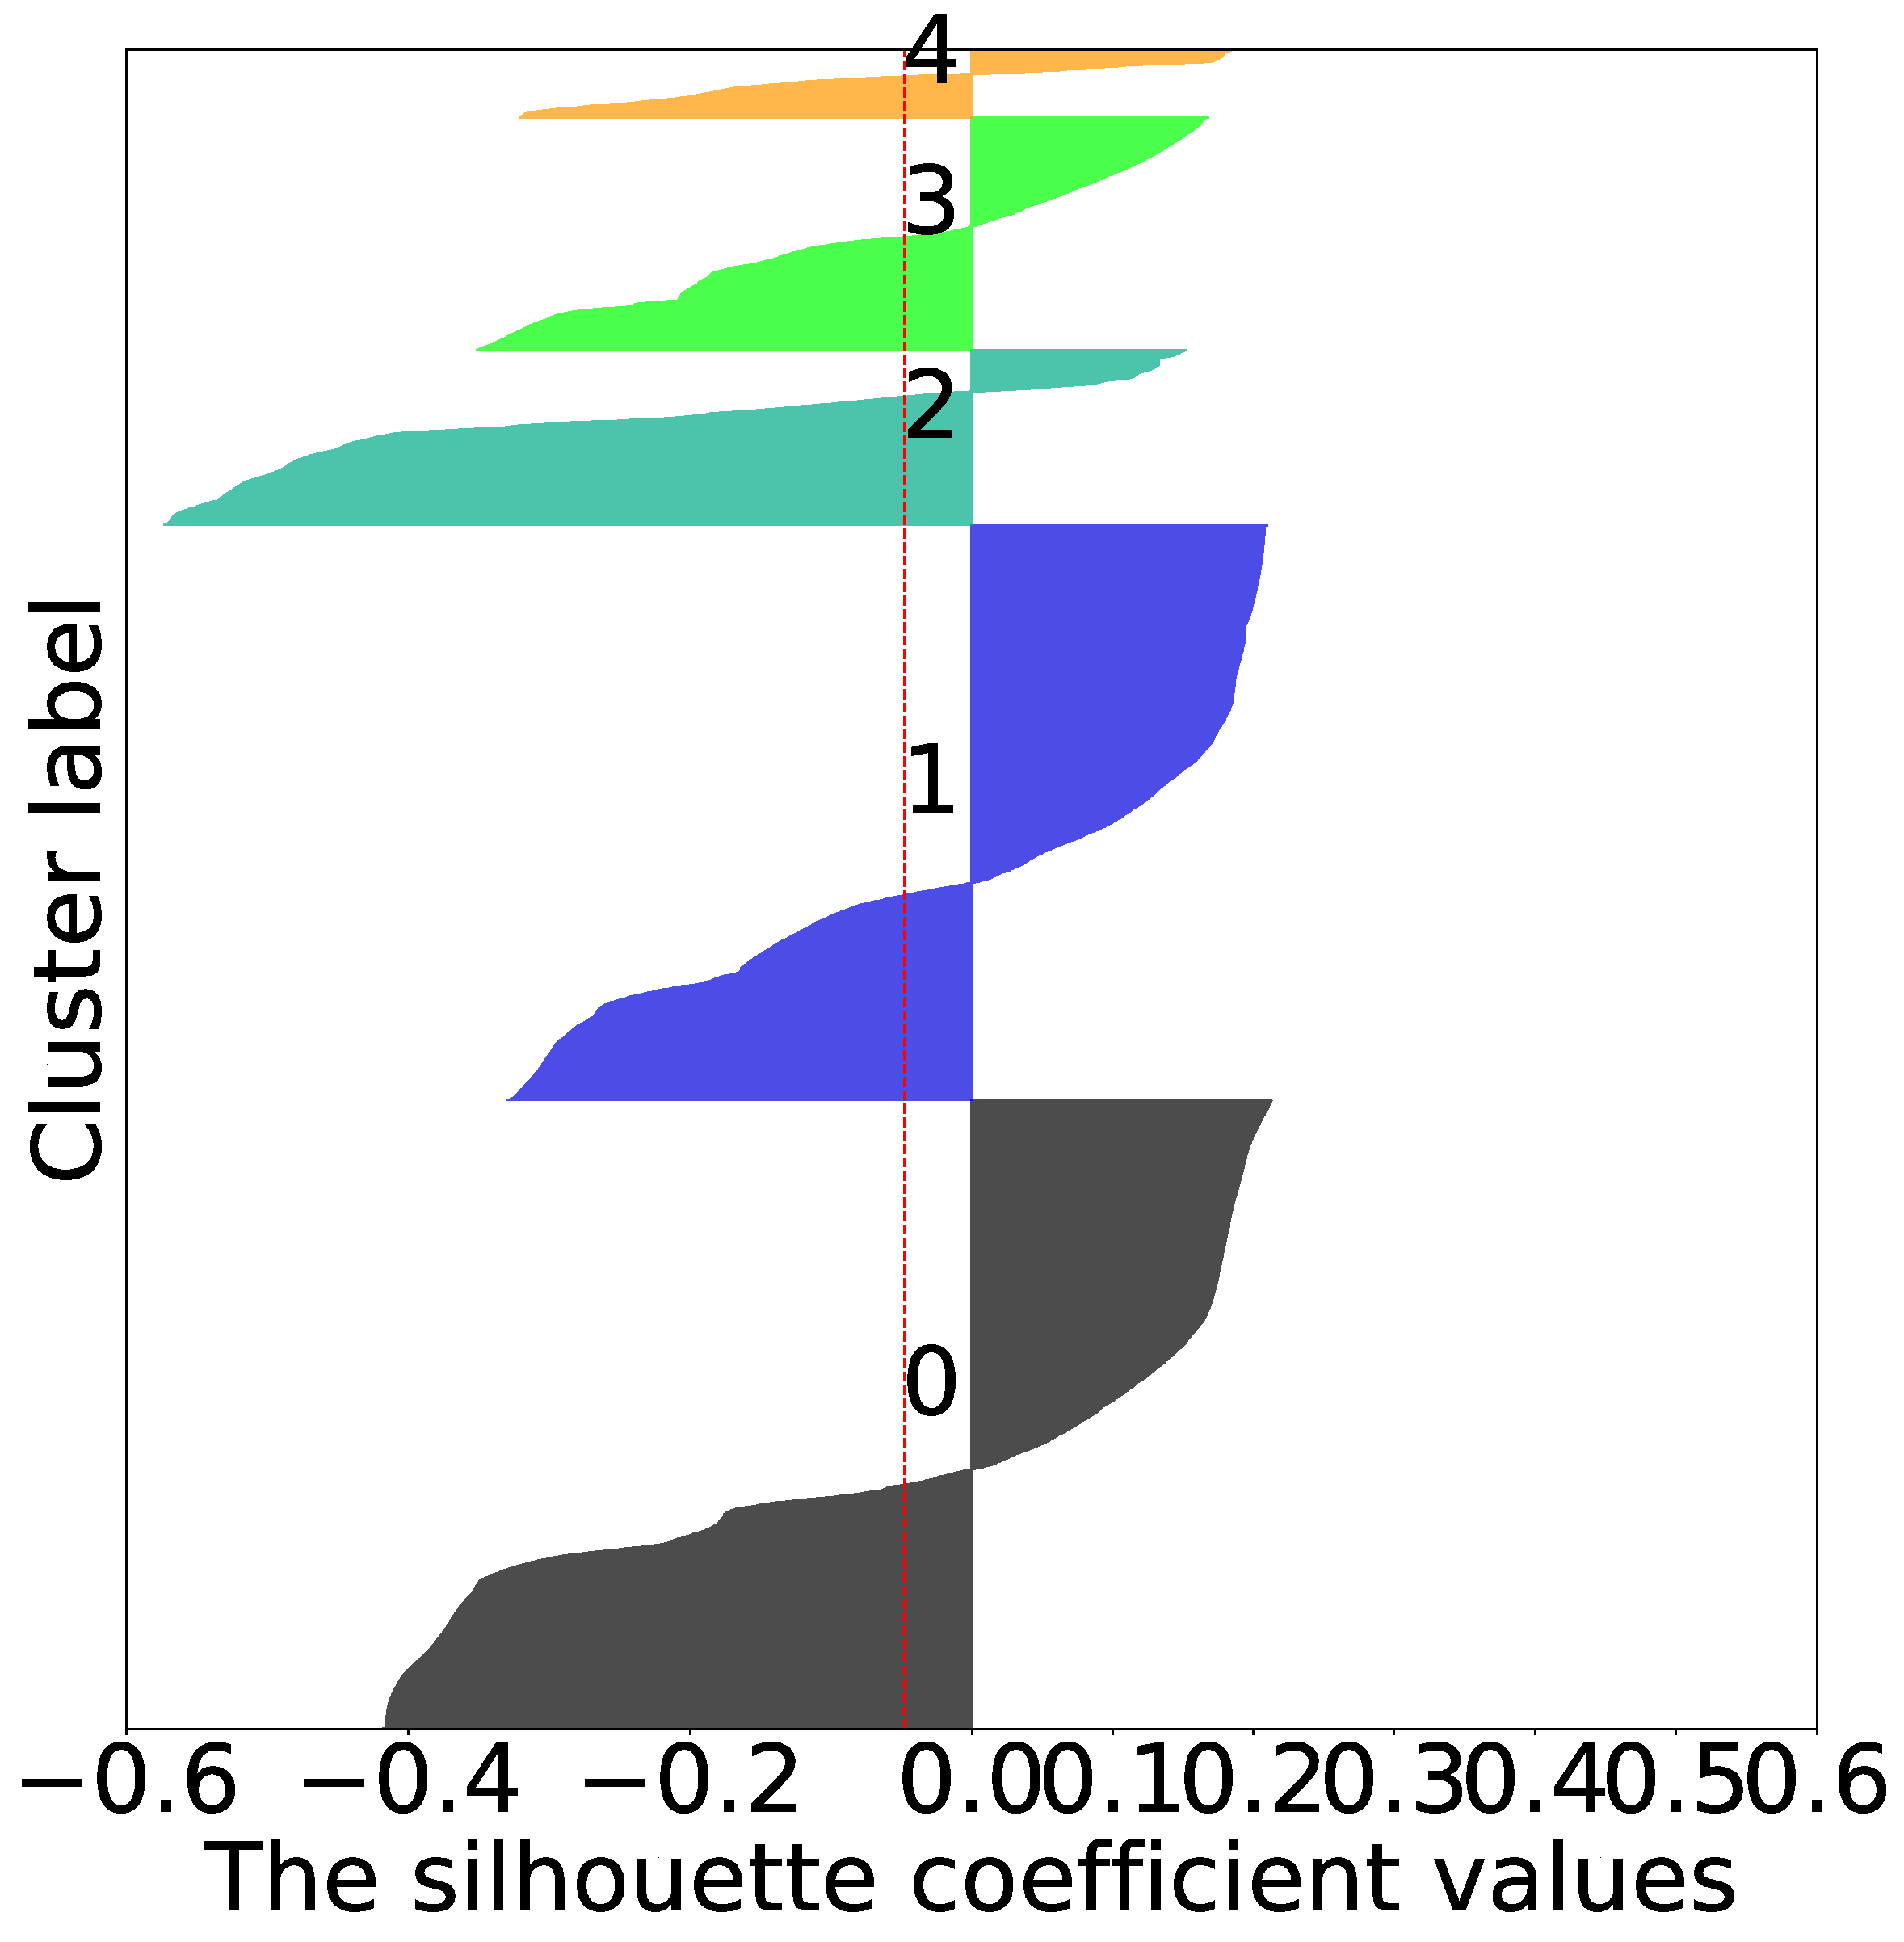
\includegraphics[width=0.45\textwidth]{figures/silhouette/silhouette_statistics_5.pdf}
    }\\
        \subfloat[n\_clusters = 6]{
        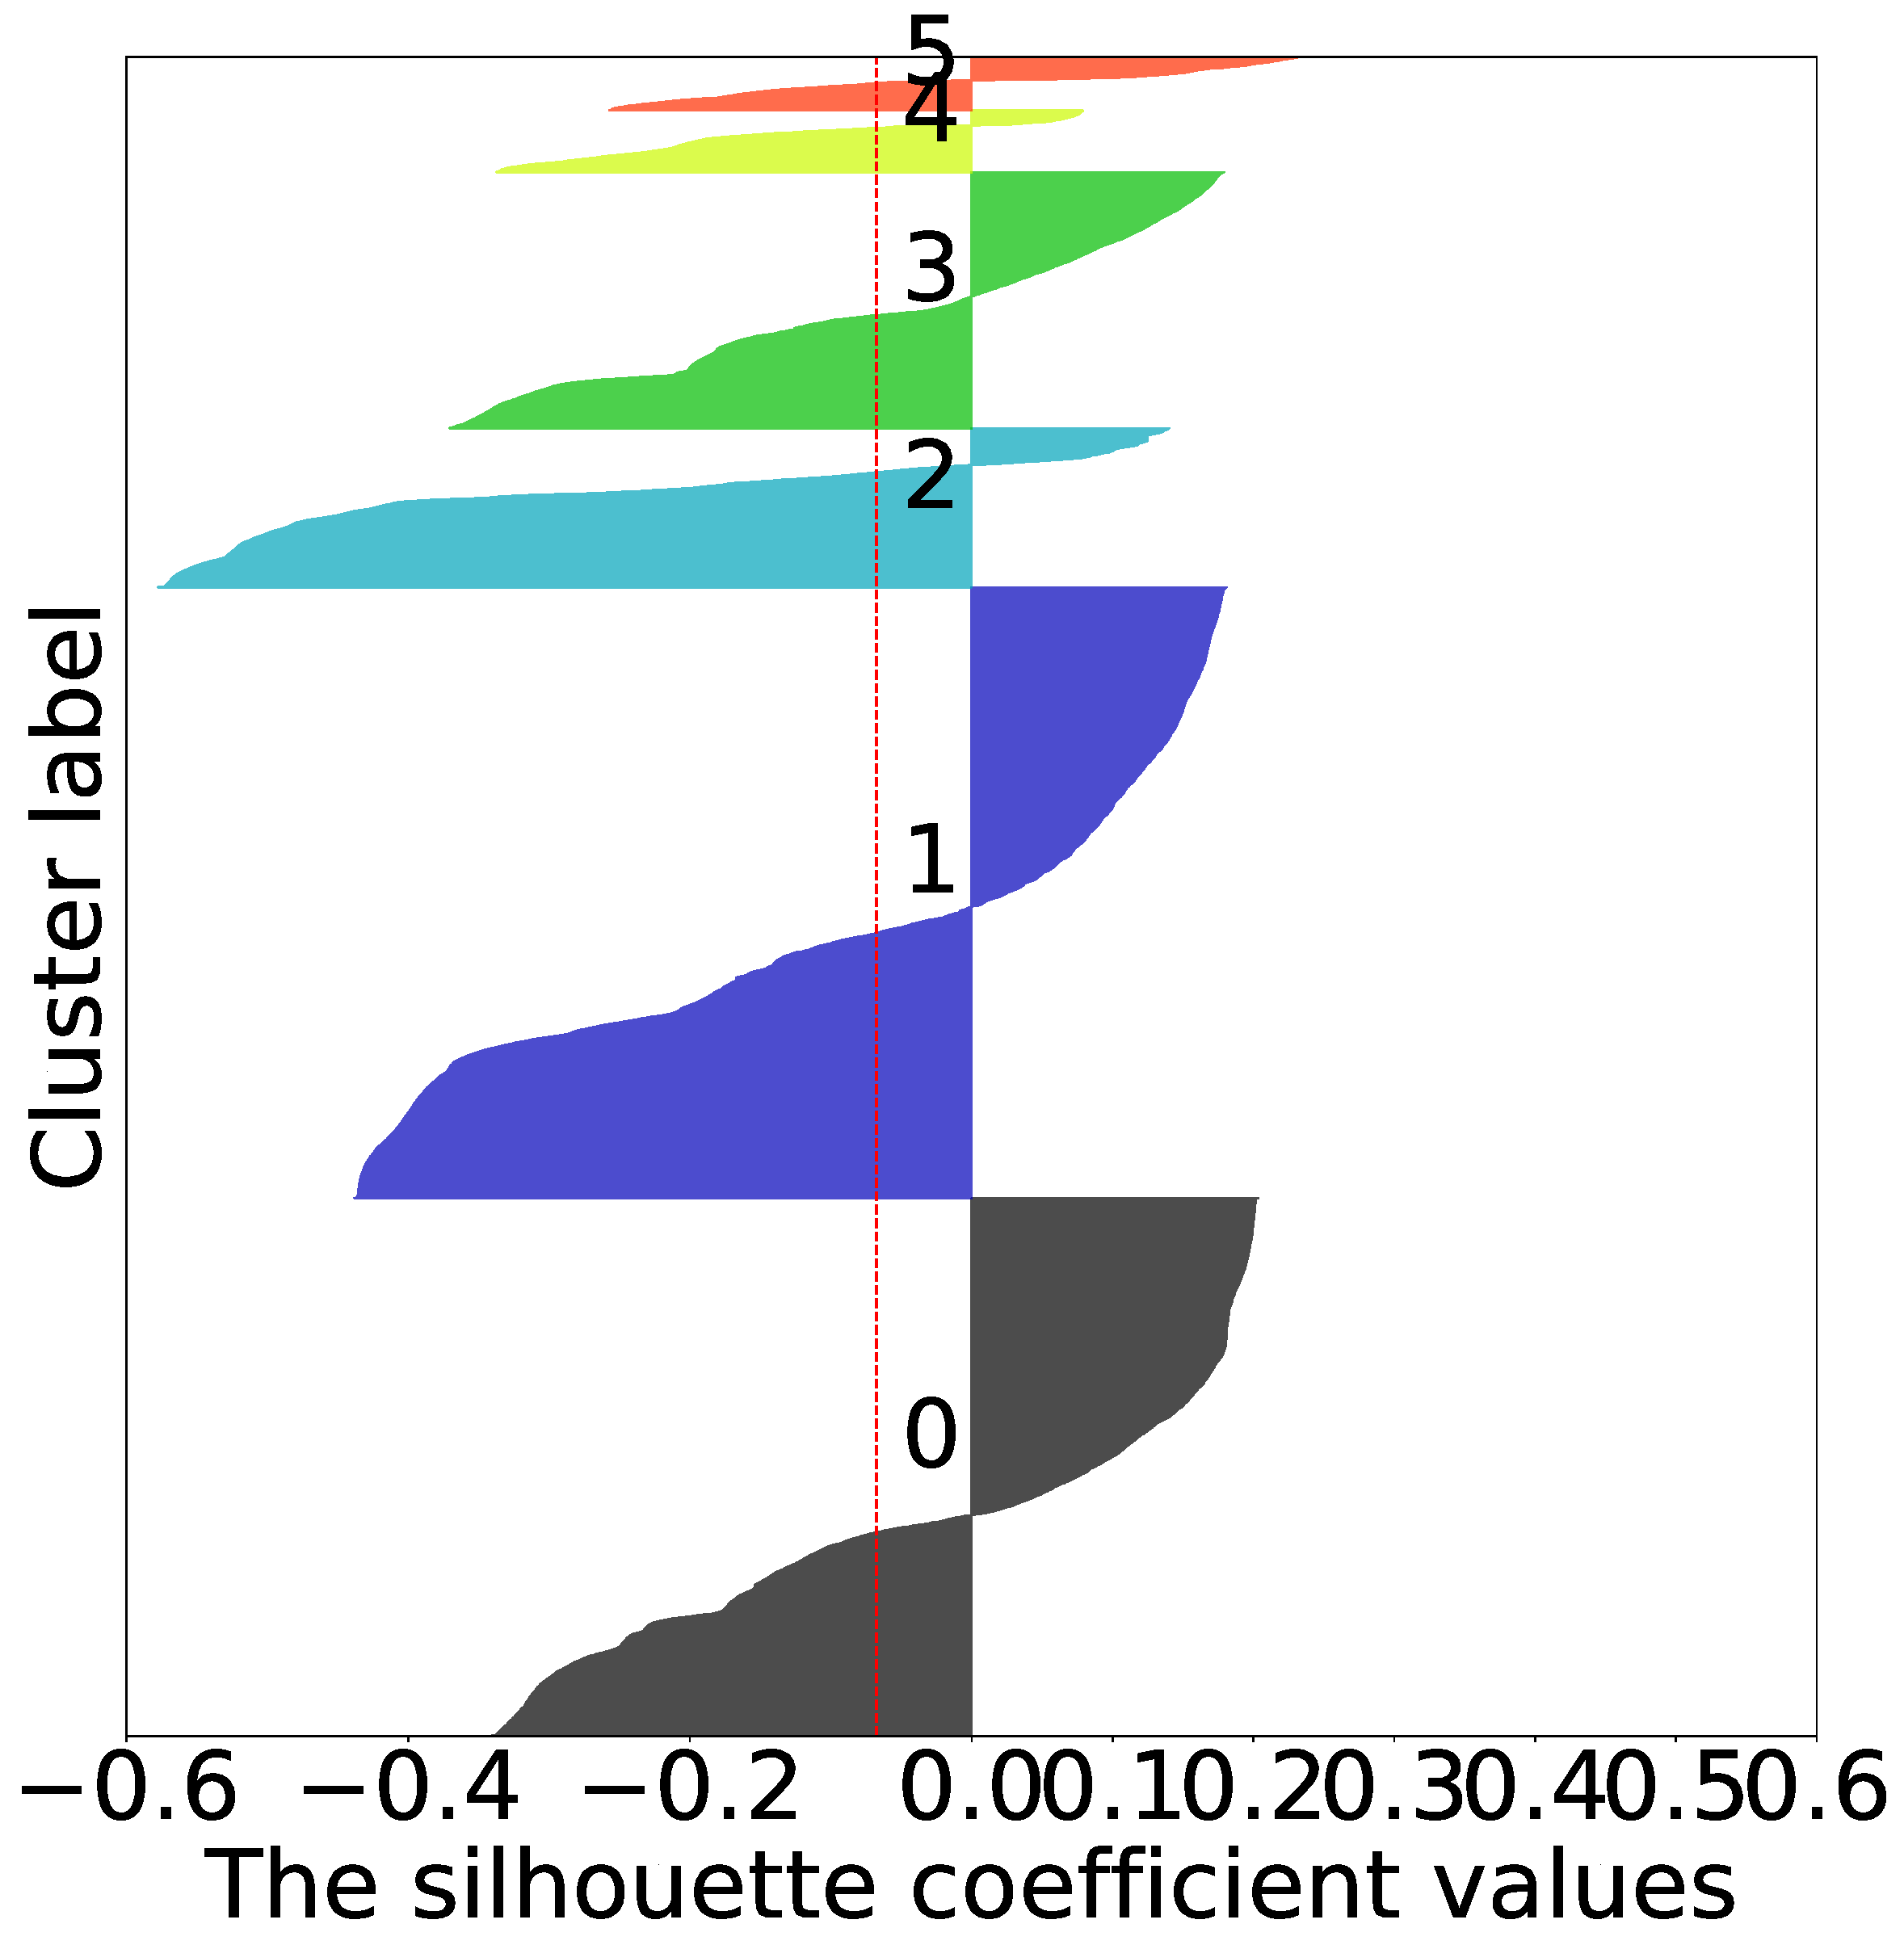
\includegraphics[width=0.45\textwidth]{figures/silhouette/silhouette_statistics_6.pdf}
    }
        \subfloat[n\_clusters = 7]{
        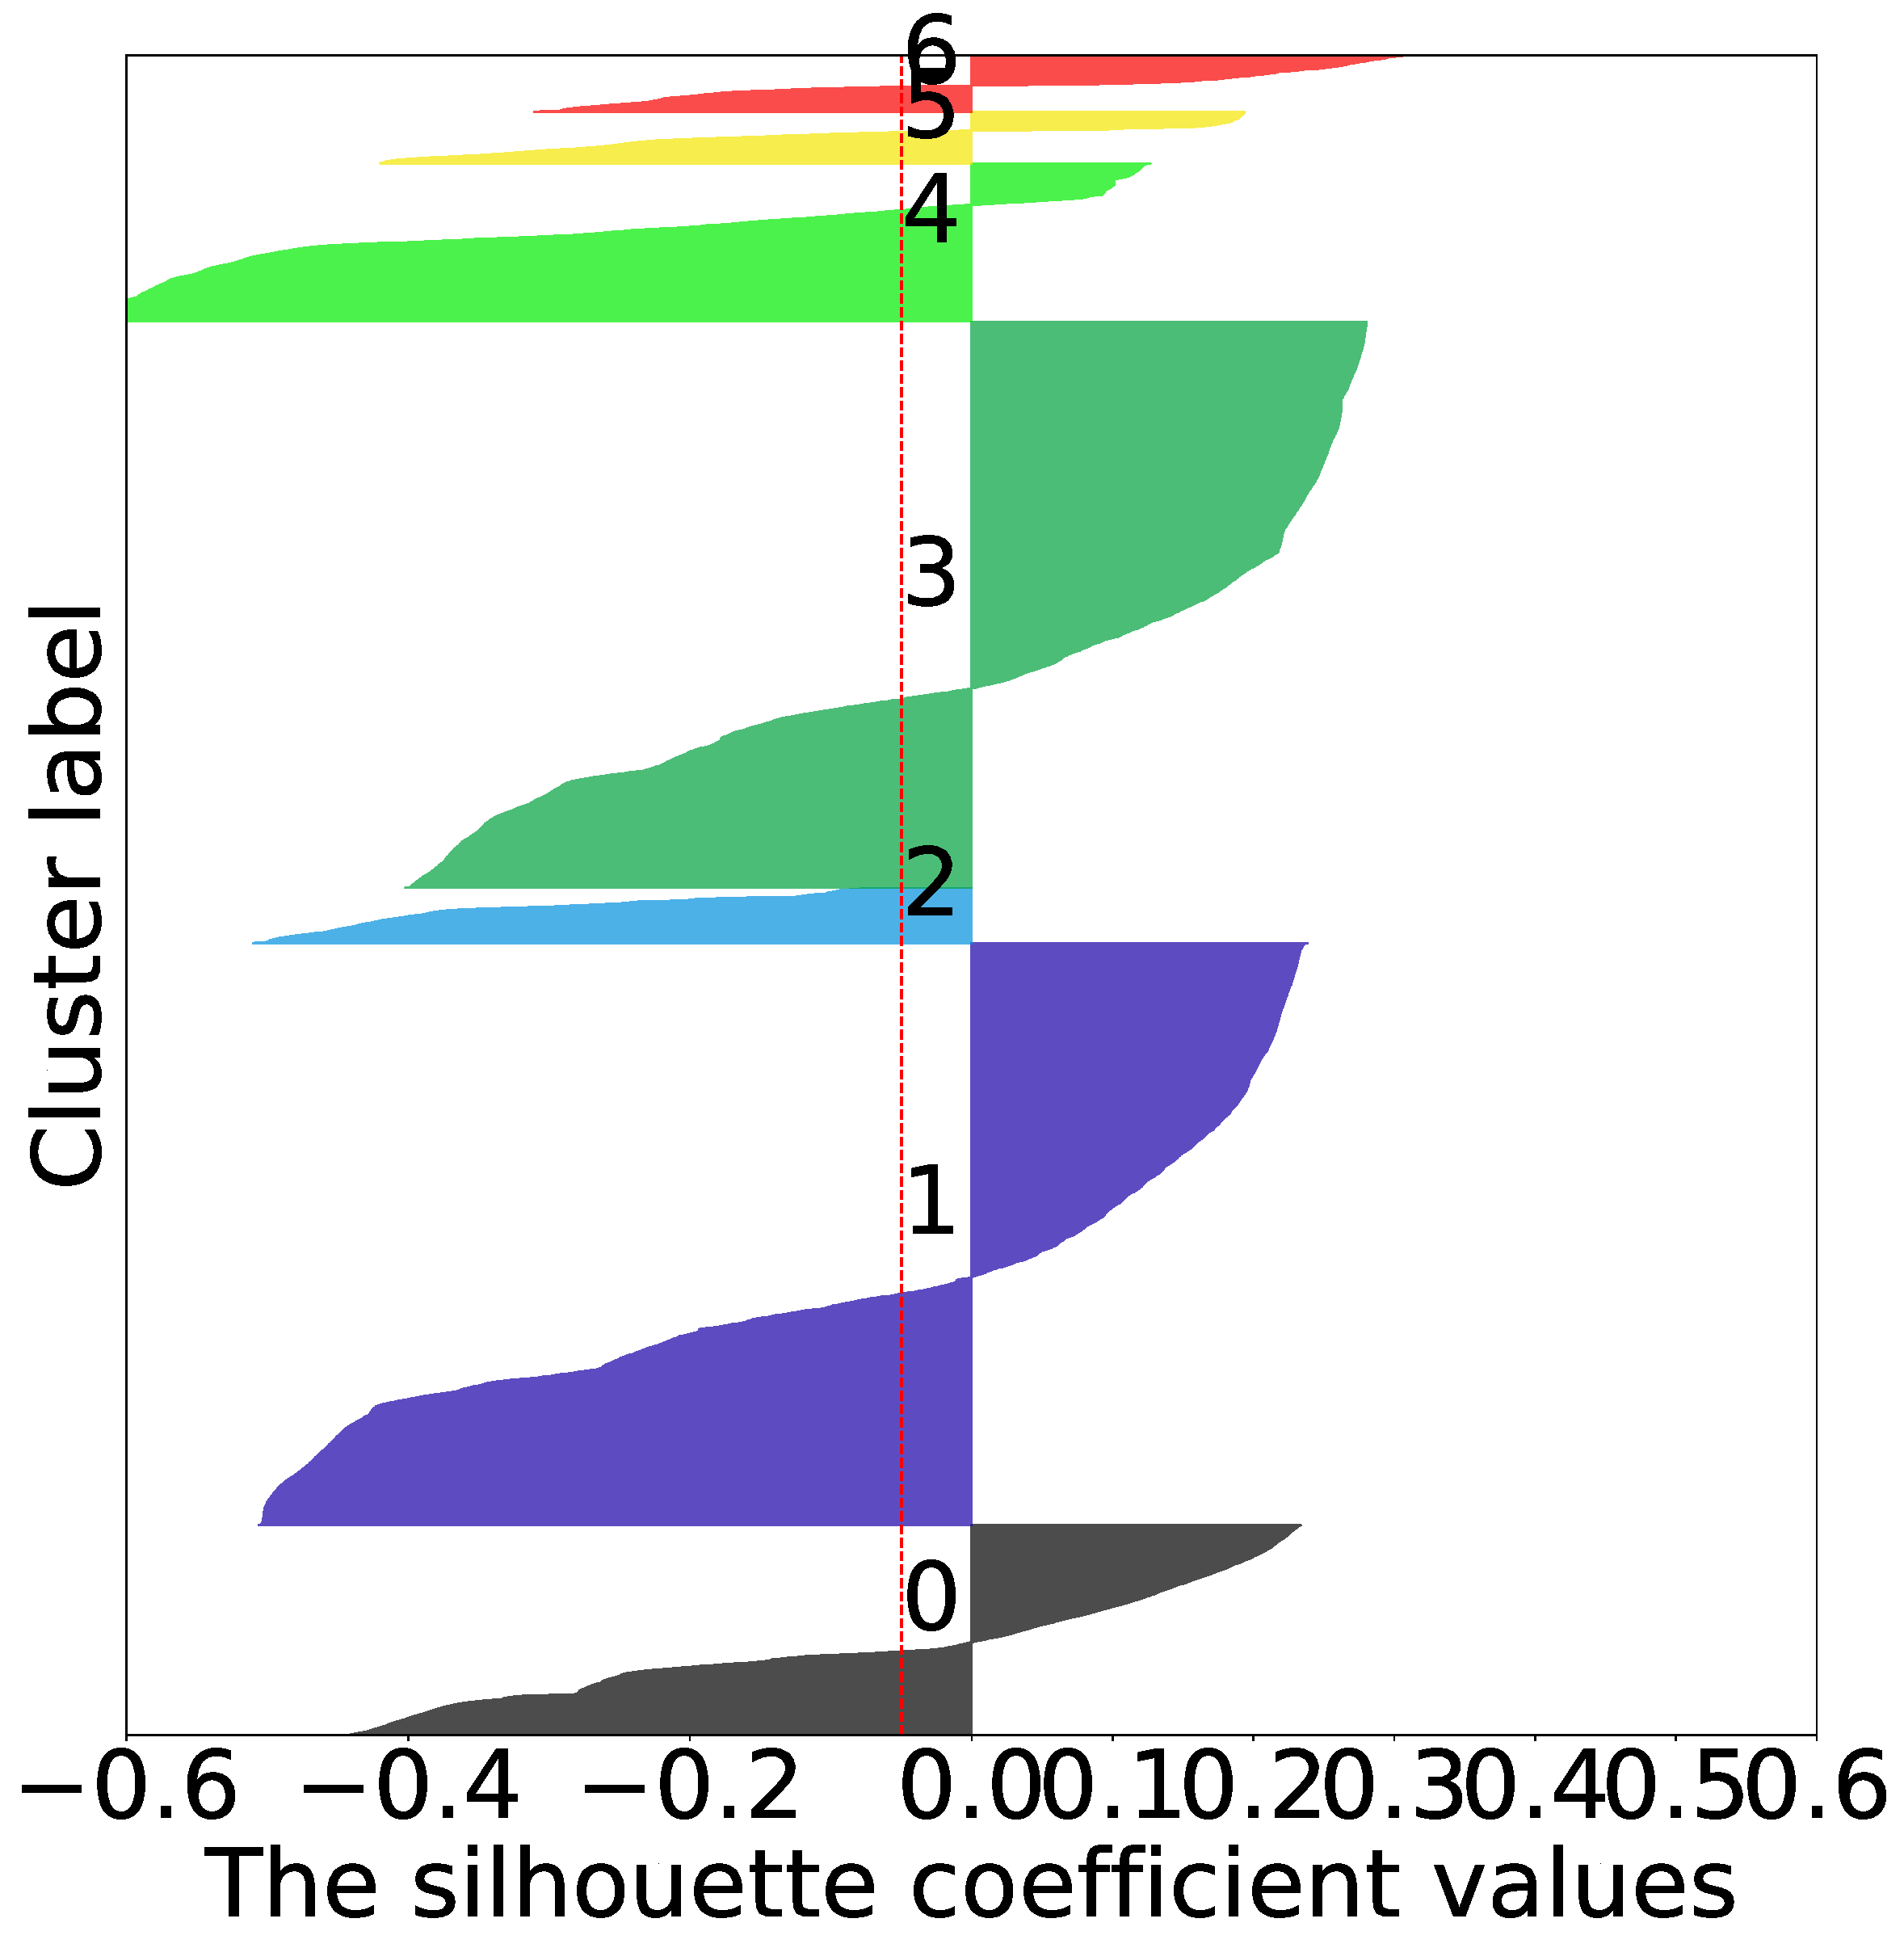
\includegraphics[width=0.45\textwidth]{figures/silhouette/silhouette_statistics_7.pdf}
    }
    \caption{Silhouette analysis of KMeans on windowed GPU load statistics}
    \label{fig_silhouette_statistics}
\end{figure}

Ultimately, we used more descriptive statistics to help understand its central tendency, spread, and shape to aid alerting. We can use nine descriptive statistics metrics to provide valuable insights into the characteristics of the data: percentiles (25\%, 50\%, 75\%), kurtosis, maximum, minimum, skewness, standard deviation, and variance, as defined in Subsection \ref{subsec:statistics}.

Figure \ref{fig_load_gpu_histogram_1} and Figure \ref{fig_load_gpu_histogram_2} show the histogram distribution graph. The graph shows that kurtosis, mean, skewness, and standard deviation have a central tendency. We cannot find a good separation for these data, so these metrics cannot separate good and bad jobs. Combined with the analysis of the monitoring data in production and the actual need for job alerting, which is to find out the bad jobs that can be significantly improved, we eventually fine-tuned and discovered that 20 in the 75th percentile and 32 in the maximum are good separations, as defined in Algorithm \ref{algo:statistics}.

\begin{algorithm}[H]
\SetAlgoLined
\KwData{Array, Fixed-size sliding window of latest GPU usage history: $A$}
\KwResult{Boolean, indicating if an alert should be raised}
\SetKwFunction{FMain}{checkAlert}
\SetKwFunction{FPercentile}{getPercentile}
\SetKwProg{Fn}{Function}{:}{}

\Fn{\FPercentile{$array$, $divide$}}{
    \Return $array[\lfloor(\text{len}(array) - 1) / divide\rfloor]$\;
}

\Fn{\FMain{$A$}}{
    $array \leftarrow$ Sort $A$ in ascending order\;
    $P_{75} \leftarrow \FPercentile(array, \frac{4}{3})$\;
    $M \leftarrow \FPercentile(array, 1)$\;
    \If{$P_{75} < 20$ \textbf{or} $M < 32$}{
        \Return true\;
    }
    \Else{
        \Return false\;
    }
}

\caption{Checking GPU load alert based on percentile and maximum}
\label{algo:statistics}
\end{algorithm}

\begin{figure}[H]
    \centering
        \subfloat[25\%]{
        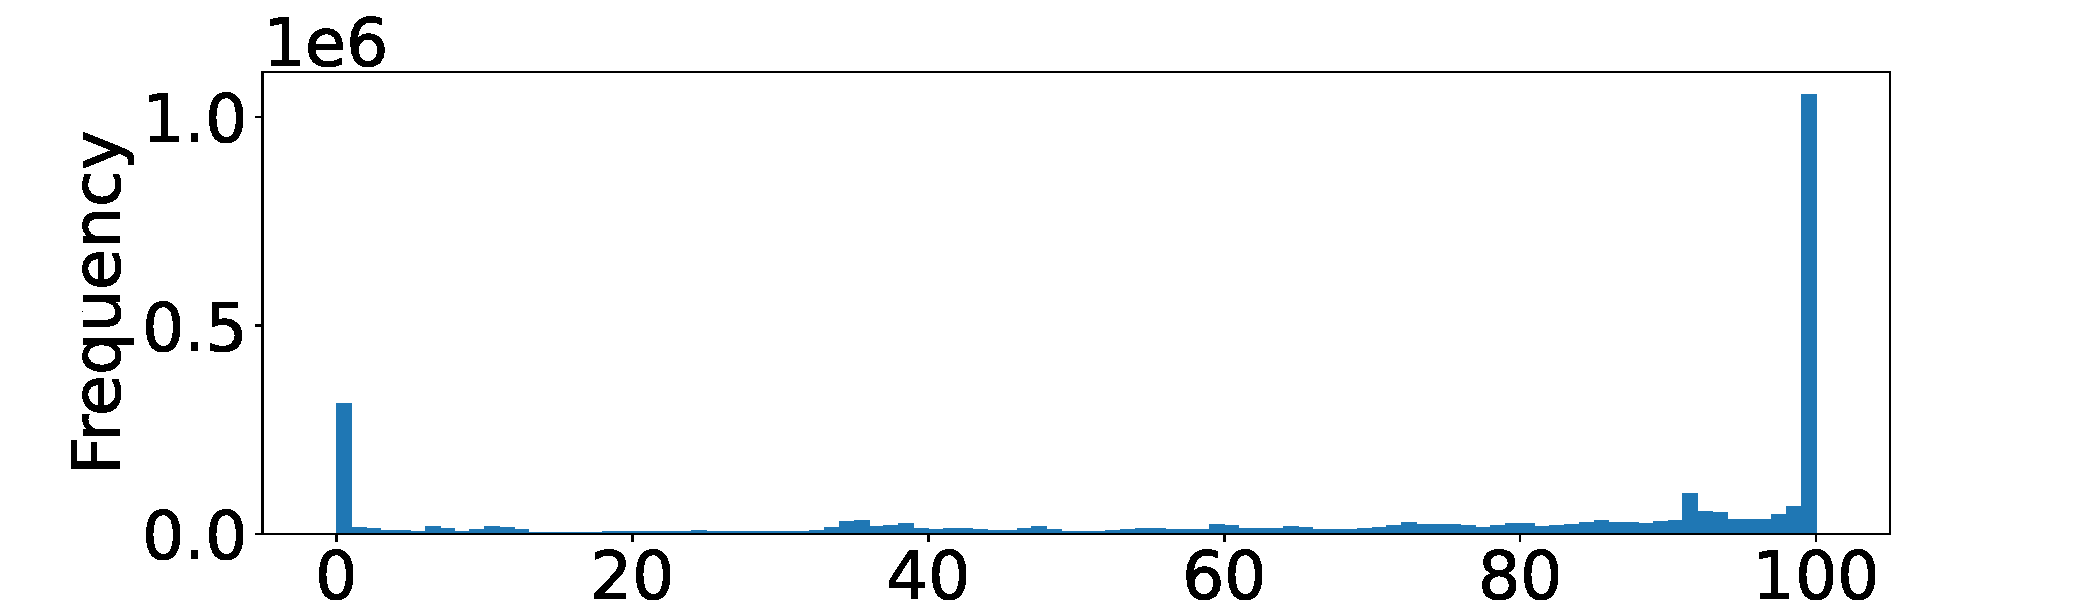
\includegraphics[width=0.8\textwidth]{figures/analysis/load_gpu_25_histogram.pdf}
    }\\
        \subfloat[50\%]{
        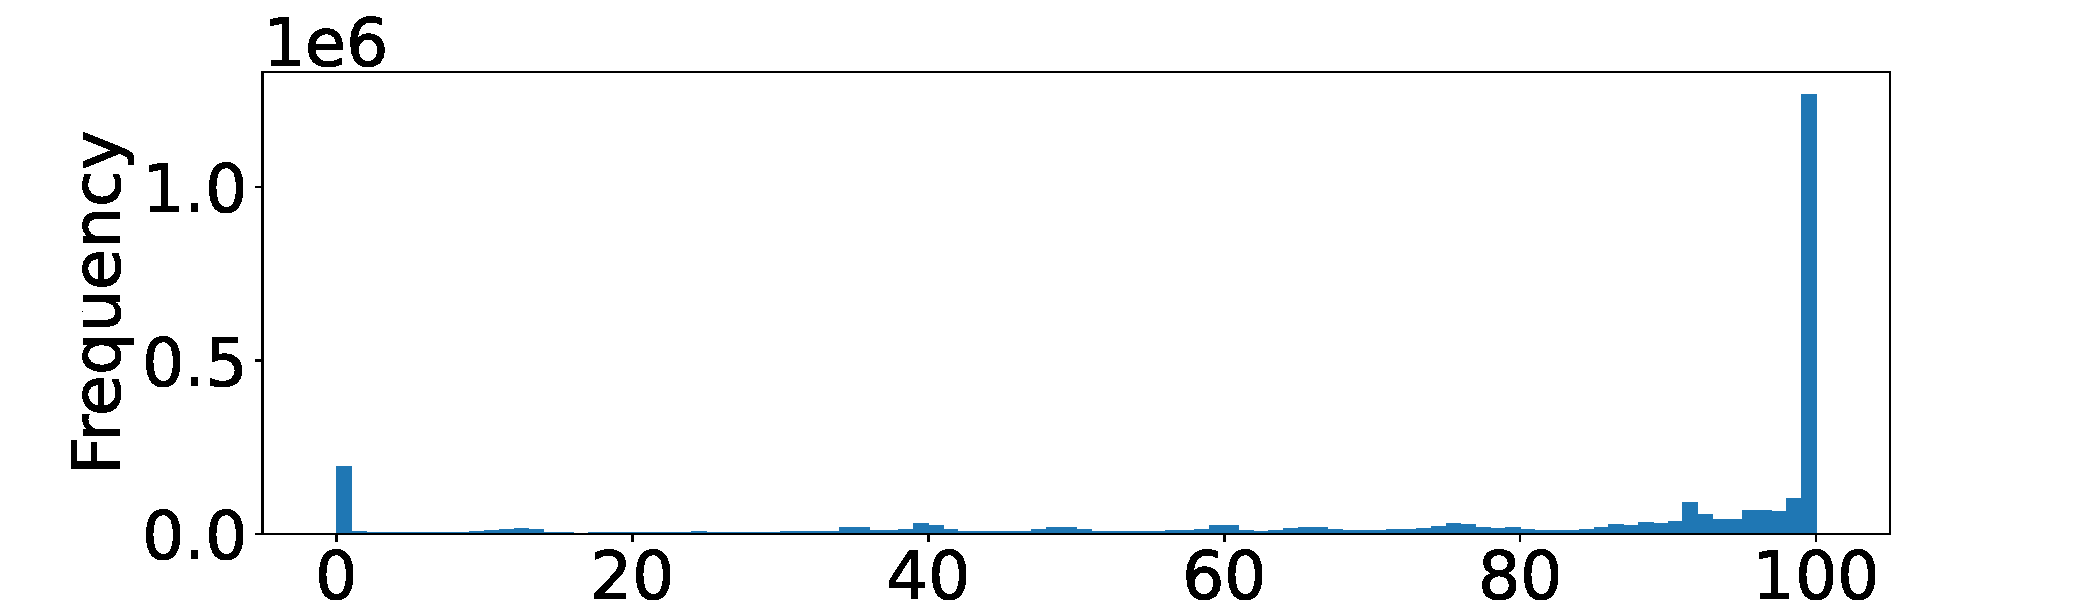
\includegraphics[width=0.8\textwidth]{figures/analysis/load_gpu_50_histogram.pdf}
    }\\
        \subfloat[75\%]{
        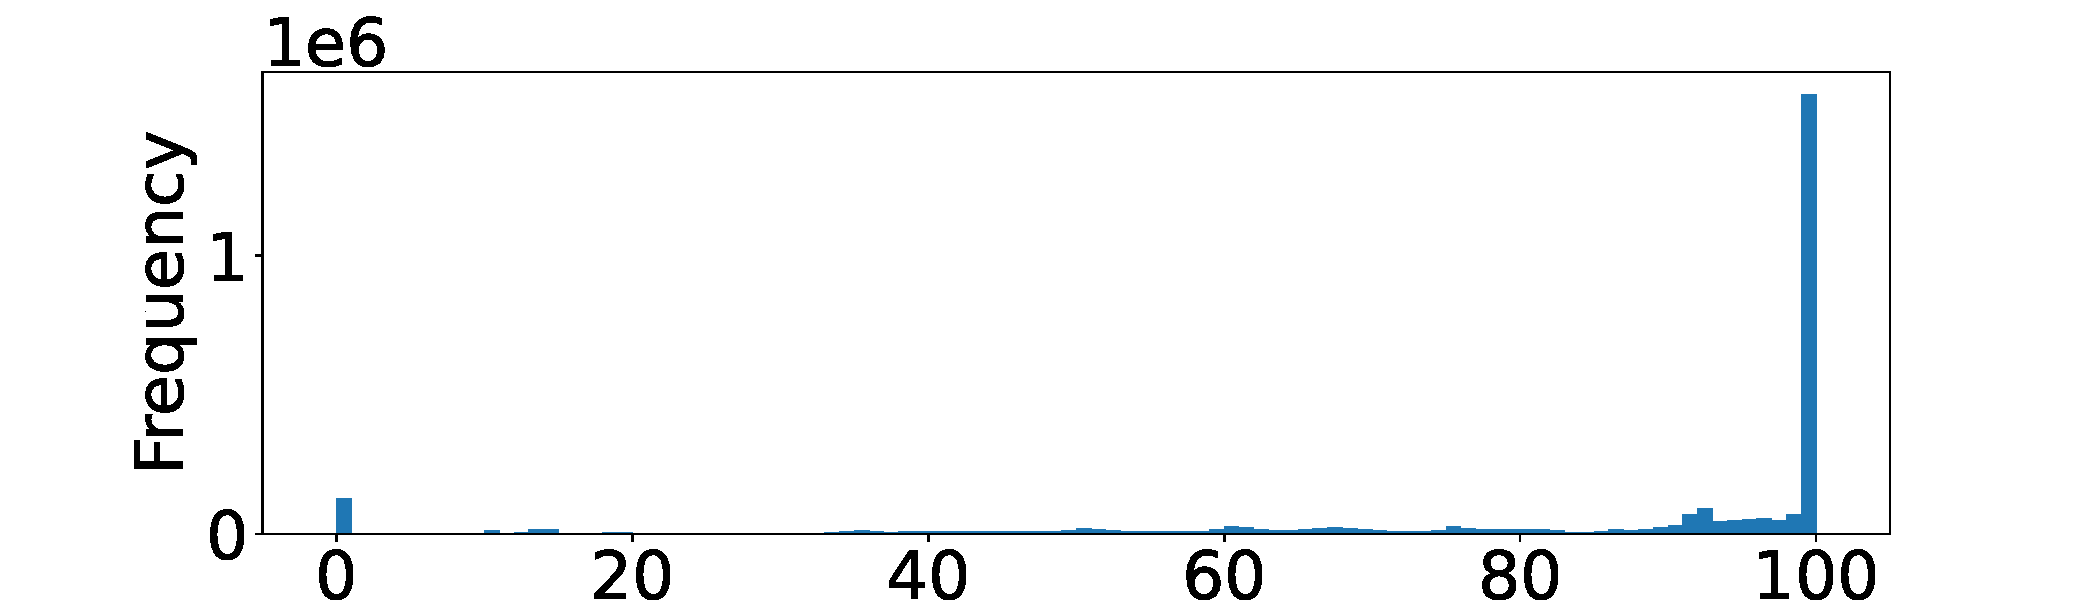
\includegraphics[width=0.8\textwidth]{figures/analysis/load_gpu_75_histogram.pdf}
    }\\
        \subfloat[Kurtosis]{
        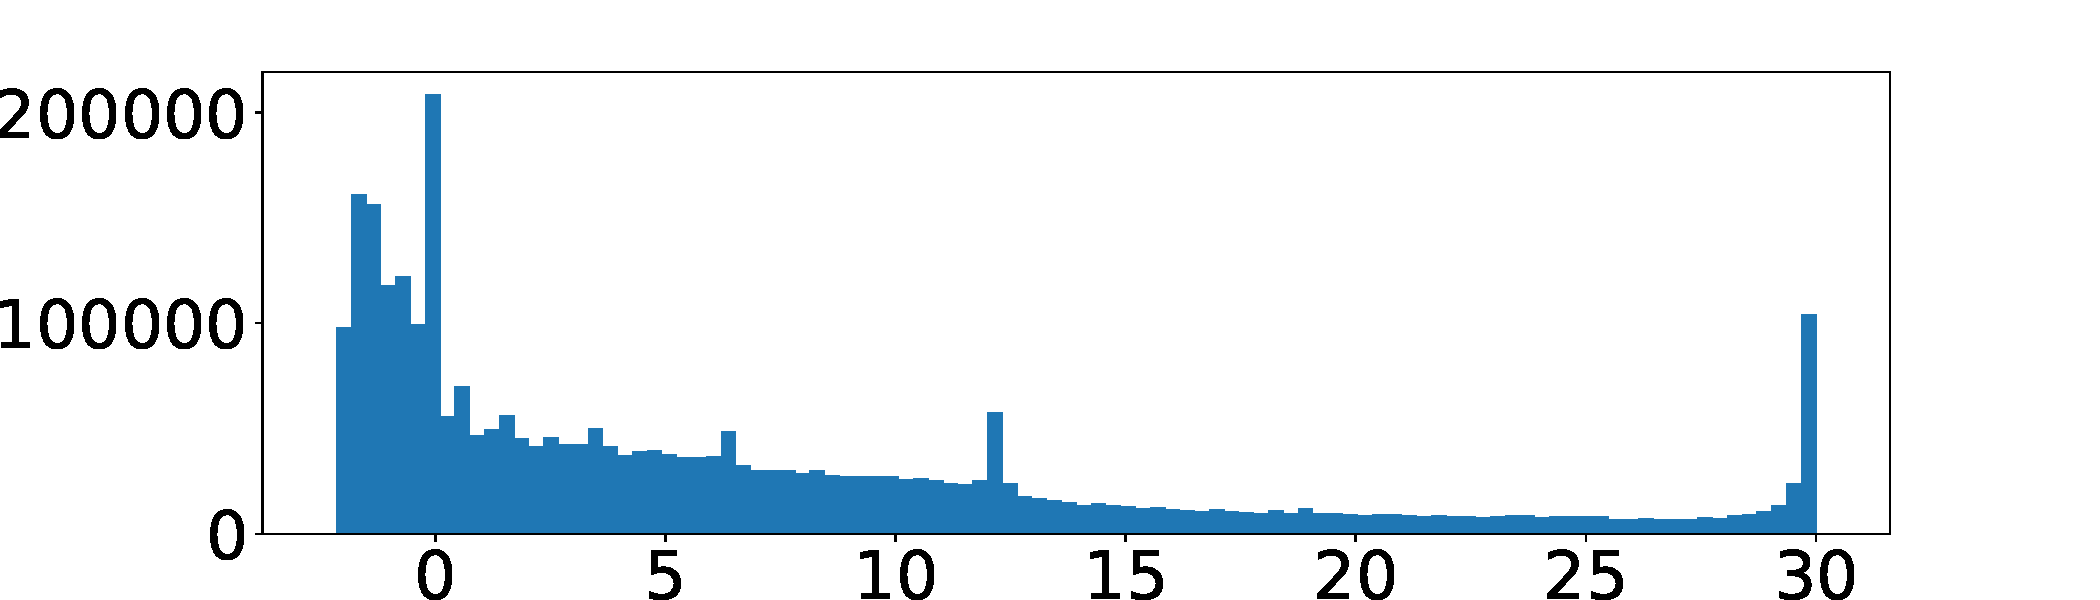
\includegraphics[width=0.8\textwidth]{figures/analysis/load_gpu_kurt_histogram.pdf}
    }\\
        \subfloat[Maximum]{
        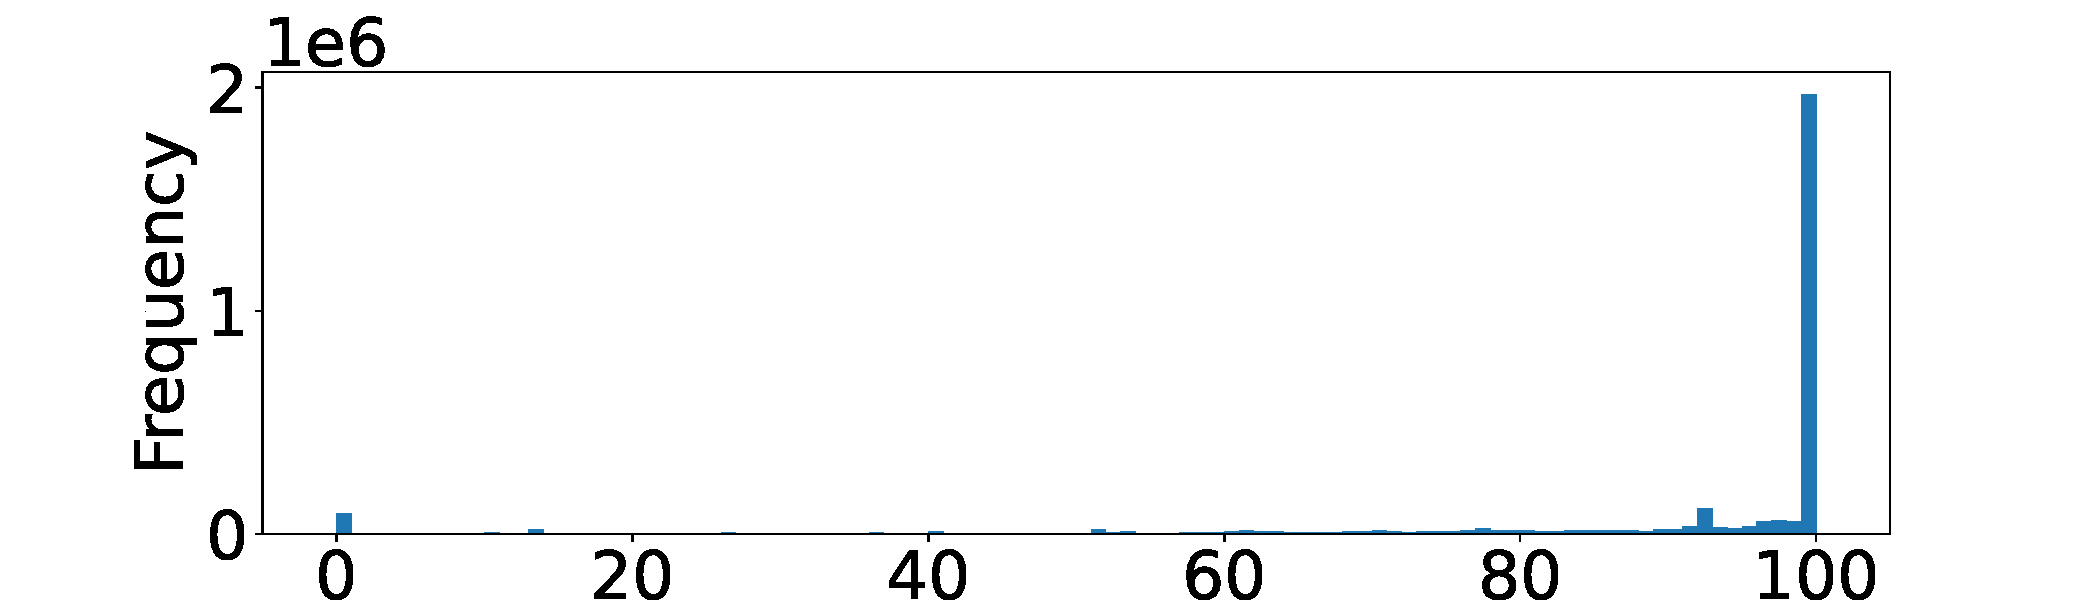
\includegraphics[width=0.8\textwidth]{figures/analysis/load_gpu_max_histogram.pdf}
    }
    \caption{Histogram of statistics analysis on windowed GPU load data, Part 1}
    \label{fig_load_gpu_histogram_1}
\end{figure}

\begin{figure}[H]
    \centering
        \subfloat[Mean]{
        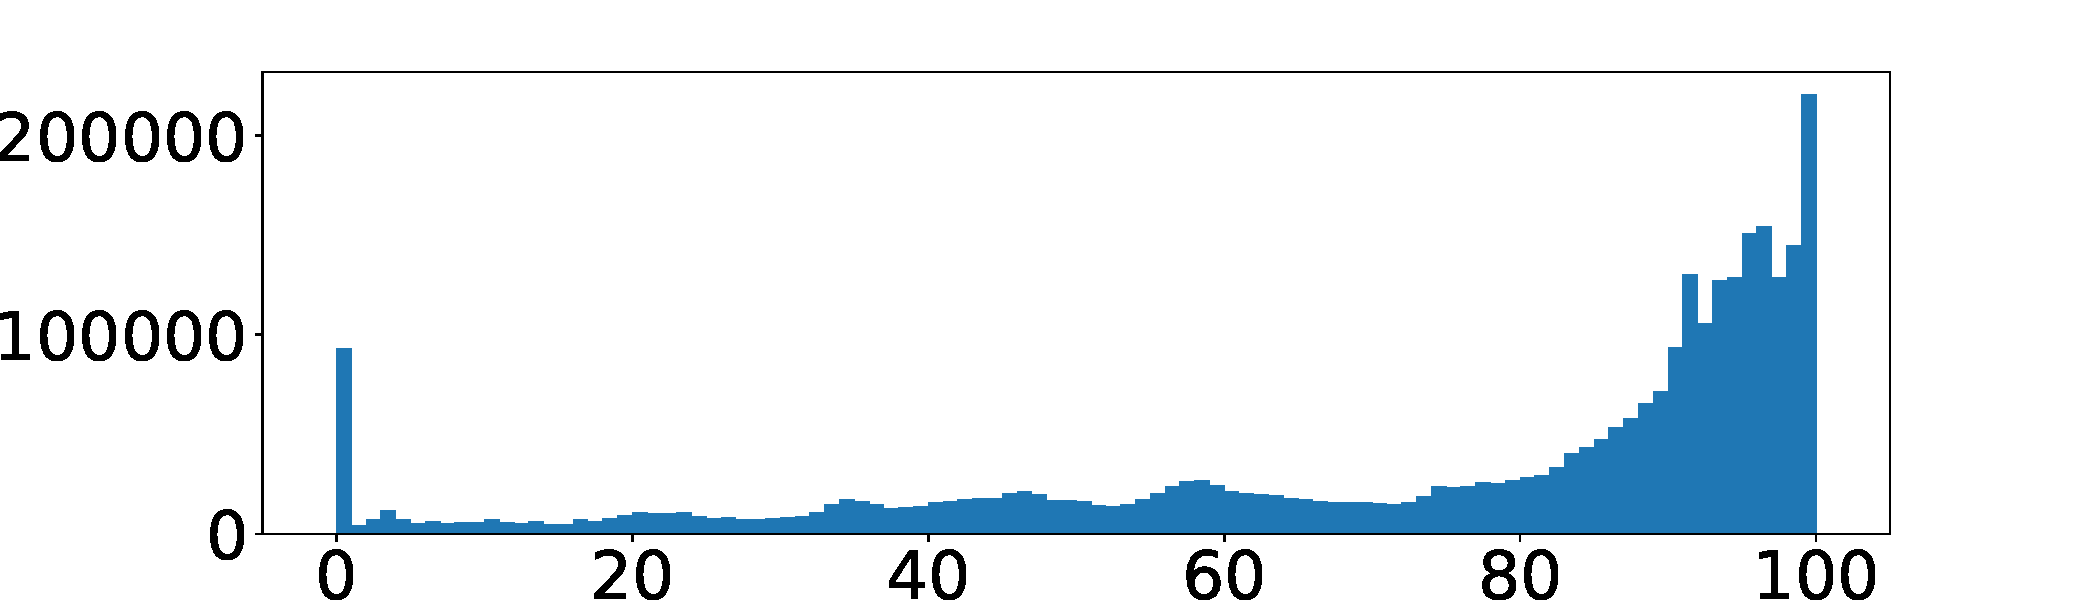
\includegraphics[width=0.8\textwidth]{figures/analysis/load_gpu_mean_histogram.pdf}
    }\\
        \subfloat[Minimum]{
        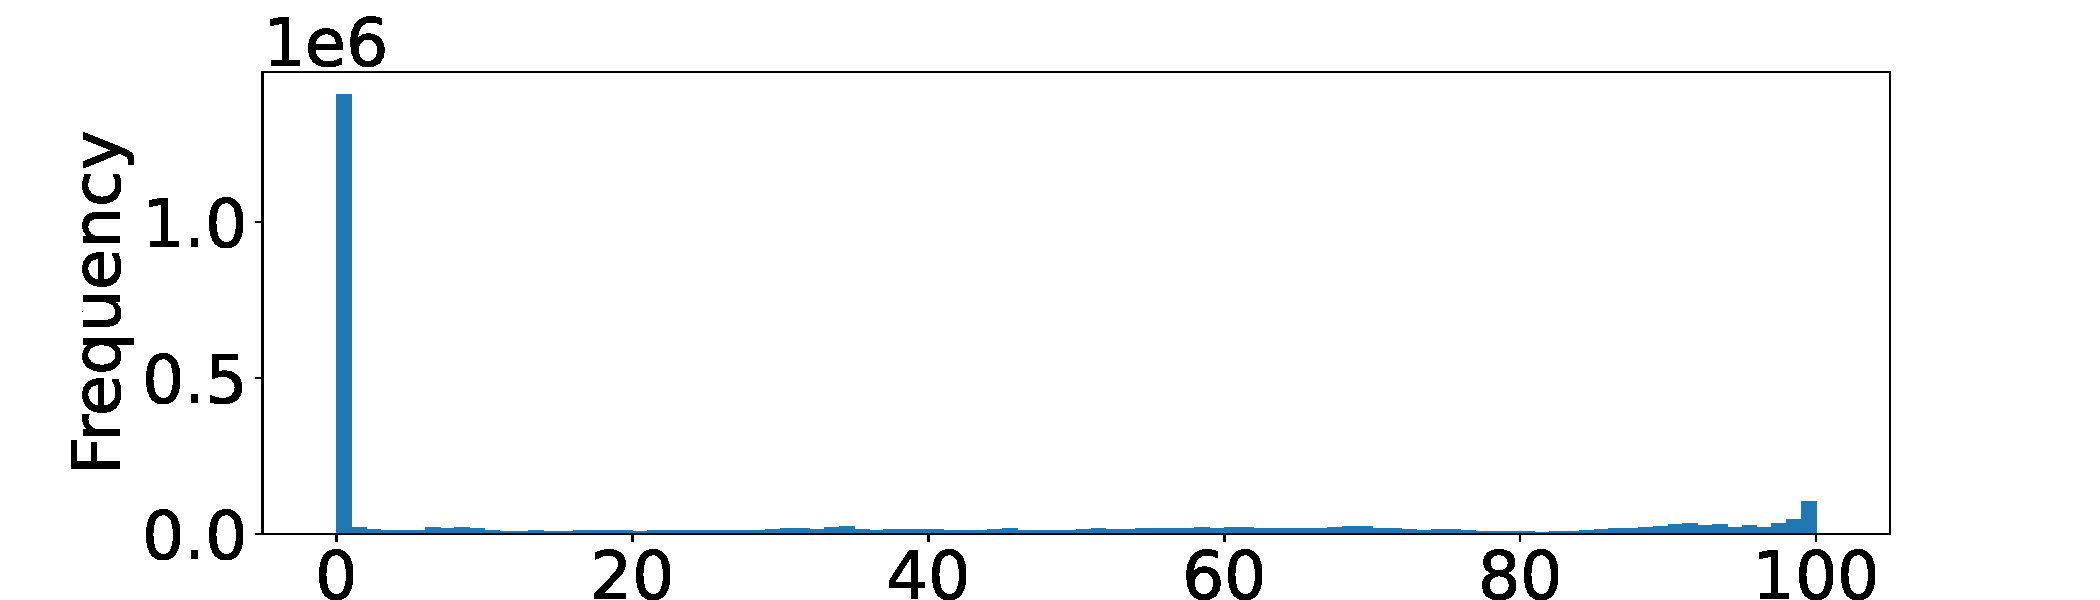
\includegraphics[width=0.8\textwidth]{figures/analysis/load_gpu_min_histogram.pdf}
    }\\
        \subfloat[Skewness]{
        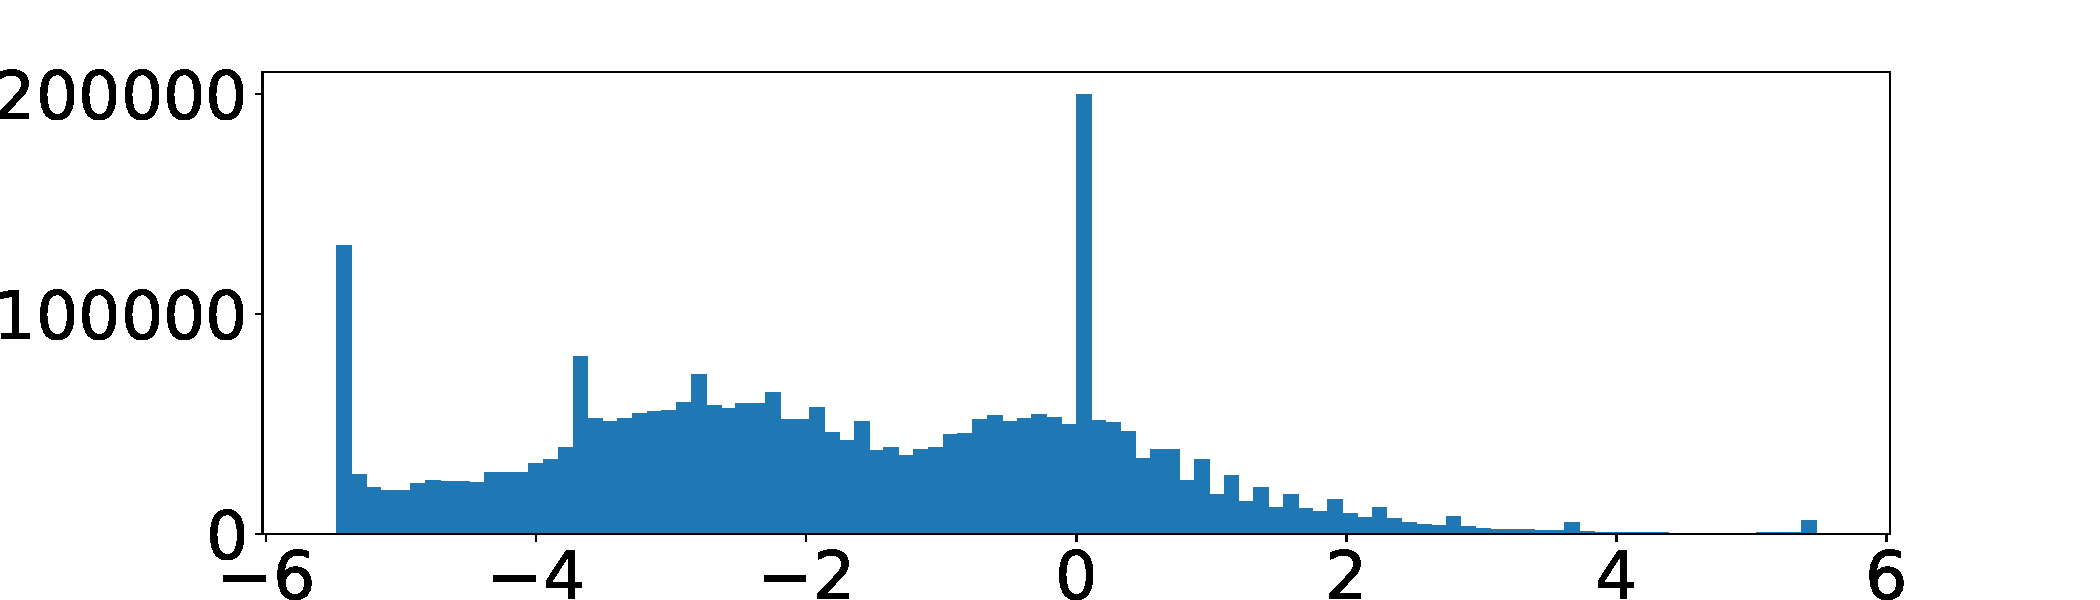
\includegraphics[width=0.8\textwidth]{figures/analysis/load_gpu_skew_histogram.pdf}
    }\\
        \subfloat[Standard deviation]{
        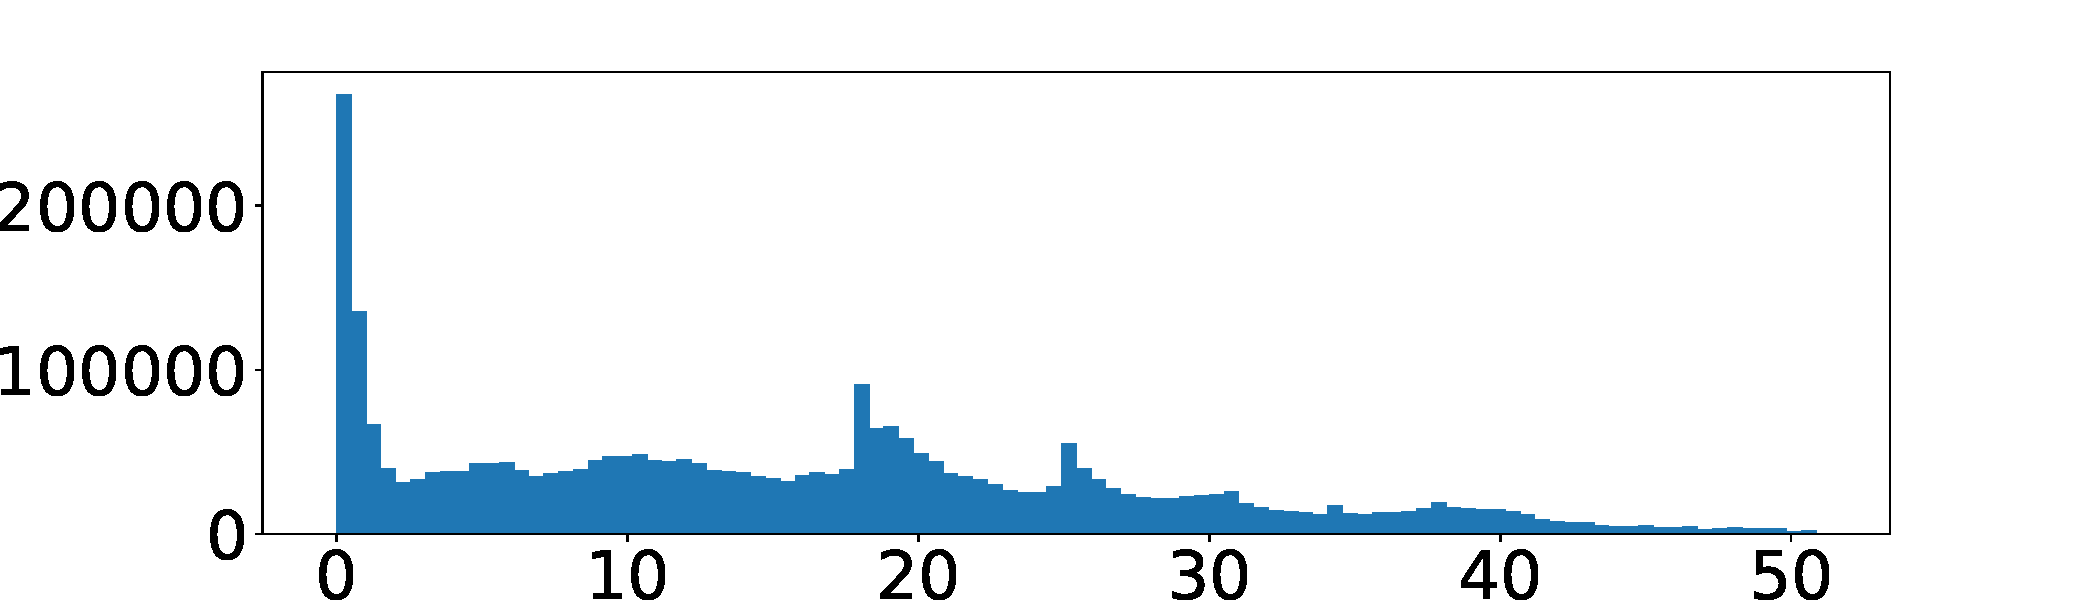
\includegraphics[width=0.8\textwidth]{figures/analysis/load_gpu_std_histogram.pdf}
    }
    \caption{Histogram of statistics analysis on windowed GPU load data, Part 2}
    \label{fig_load_gpu_histogram_2}
\end{figure}

\section{Alert service}
\label{sec:alertservice}
The alert service we implemented is built on the monitoring system. A good design is crucial for addressing all the research questions in Section \ref{sec:rqs}.

% communicates with the TimescaleDB through triggers to update the internal state in memory. 
For \textbf{maintaining the internal state} for tracking different jobs, The alert service can create or destroy the internal state for specific jobs by following job metadata updates. Whenever we have a new alert, or the alert is dismissed, we write the event into logs. We garbage collect stale jobs to avoid memory leaks. We get the aggregation result as soon as data are inserted. For the dashboard RESTful API integration, handling the one-writer, multiple-reader problem can be very complex if we directly let the API server access our internal state, as starvation can quickly happen, thus causing significantly reduced performance. In the end, we chose to convert the issue into the one-writer, one-reader problem by dumping the alert state with a thread separately at regular intervals into the JSON string, so that we can easily tackle the issue by simply using the thread-safe map and mutual exclusion lock, to solve \textbf{RQ3} in Section \ref{sec:rqs}.

For \textbf{following the job data updates}, since message queues introduce a single point of failure, and can be challenging to debug, we decided not to use them. This increases the difficulty of our design, but aside from polling, we do have an alternative: TimescaleDB, which is based on PostgreSQL. PostgreSQL has LISTEN and NOTIFY, so we can use triggers to execute NOTIFY after the insertion of each row, and Timescale Alert can LISTEN to the updates. We also have continuous aggregates in TimescaleDB \cite{ConAggs}, which can also be our choice.

As a result, we devised four solutions combining polling/triggers, and with or without continuous aggregates, to follow the job data updates, so that we can balance between \textbf{RQ1} and \textbf{RQ2} as mentioned in Section \ref{sec:rqs}.

\begin{itemize}
    \item \textbf{Polling with continuous aggregates}: Start/Stop polling as soon as job metadata updates. Use the continuous aggregates feature offered by TimescaleDB.

    \item \textbf{Polling with SQL aggregates}: Start/Stop polling as soon as job metadata updates, directly use SQL for aggregates (without using continuous aggregates for caching).

    \item \textbf{Triggers with continuous aggregates}: use the continuous aggregates feature offered by TimescaleDB and query the aggregated result according to the information sent by the \textbf{NOTIFY} as soon as the message is received.

    \item \textbf{Triggers with in-memory aggregates}: Since our monitoring system can ensure that data arrives in order and has evenly distributed intervals, we can use a fixed-size container/ring (Circular Linked List) as the sliding window to store the history data, and do the aggregation by Golang. Here, we listen to the metrics data sent by the \textbf{NOTIFY} from the database and update the internal state in memory. % We dump the internal state by a fixed interval and send the dump to the user every time the user requests the current status over API.
\end{itemize}

Here is an empirical analysis of the four design choices mentioned above: We can choose either polling or triggers. With polling, the alert delay increases and will likely burden the database heavily with read operations. The alert delay is minimized with triggers, but we might slow down the database for writing operations because of the transactional overhead.

For continuous aggregates in TimescaleDB, Spark \cite{10.1145/2783258.2789993}, and Flink \cite{10.14778/3137765.3137777}, after investigation, we found they do not have sliding-window aggregation support with a high-level API:

Since we want real-time alerts, we want to aggregate with a fixed-size sliding window that considers the latest data and drops the old data at any time, as shown in Figure \ref{fig_sliding_window}. However, TimescaleDB continuous aggregates, Spark, and Flink high-level API can only aggregate with a fixed start time, as shown in Figure \ref{fig_fixed_sliding_window}, which will work badly if we want to check the latest aggregation result at o'clock in this case since we will only have one data to aggregate in that window (only data at 11 o'clock as shown in the figure). Then, it is not very sensible to have an aggregation. Although the sliding window is not supported, we can overcome this issue by using a weighted average on the last two windows. However, it is still not a good candidate since triggers for continuous aggregates are not supported currently, as confirmed by the issue the author opened\footnote{https://github.com/timescale/timescaledb/issues/6500}. So we will have to burden the database by polling, which means many read operations plus many background jobs.

\begin{figure}[H]
    \centering
    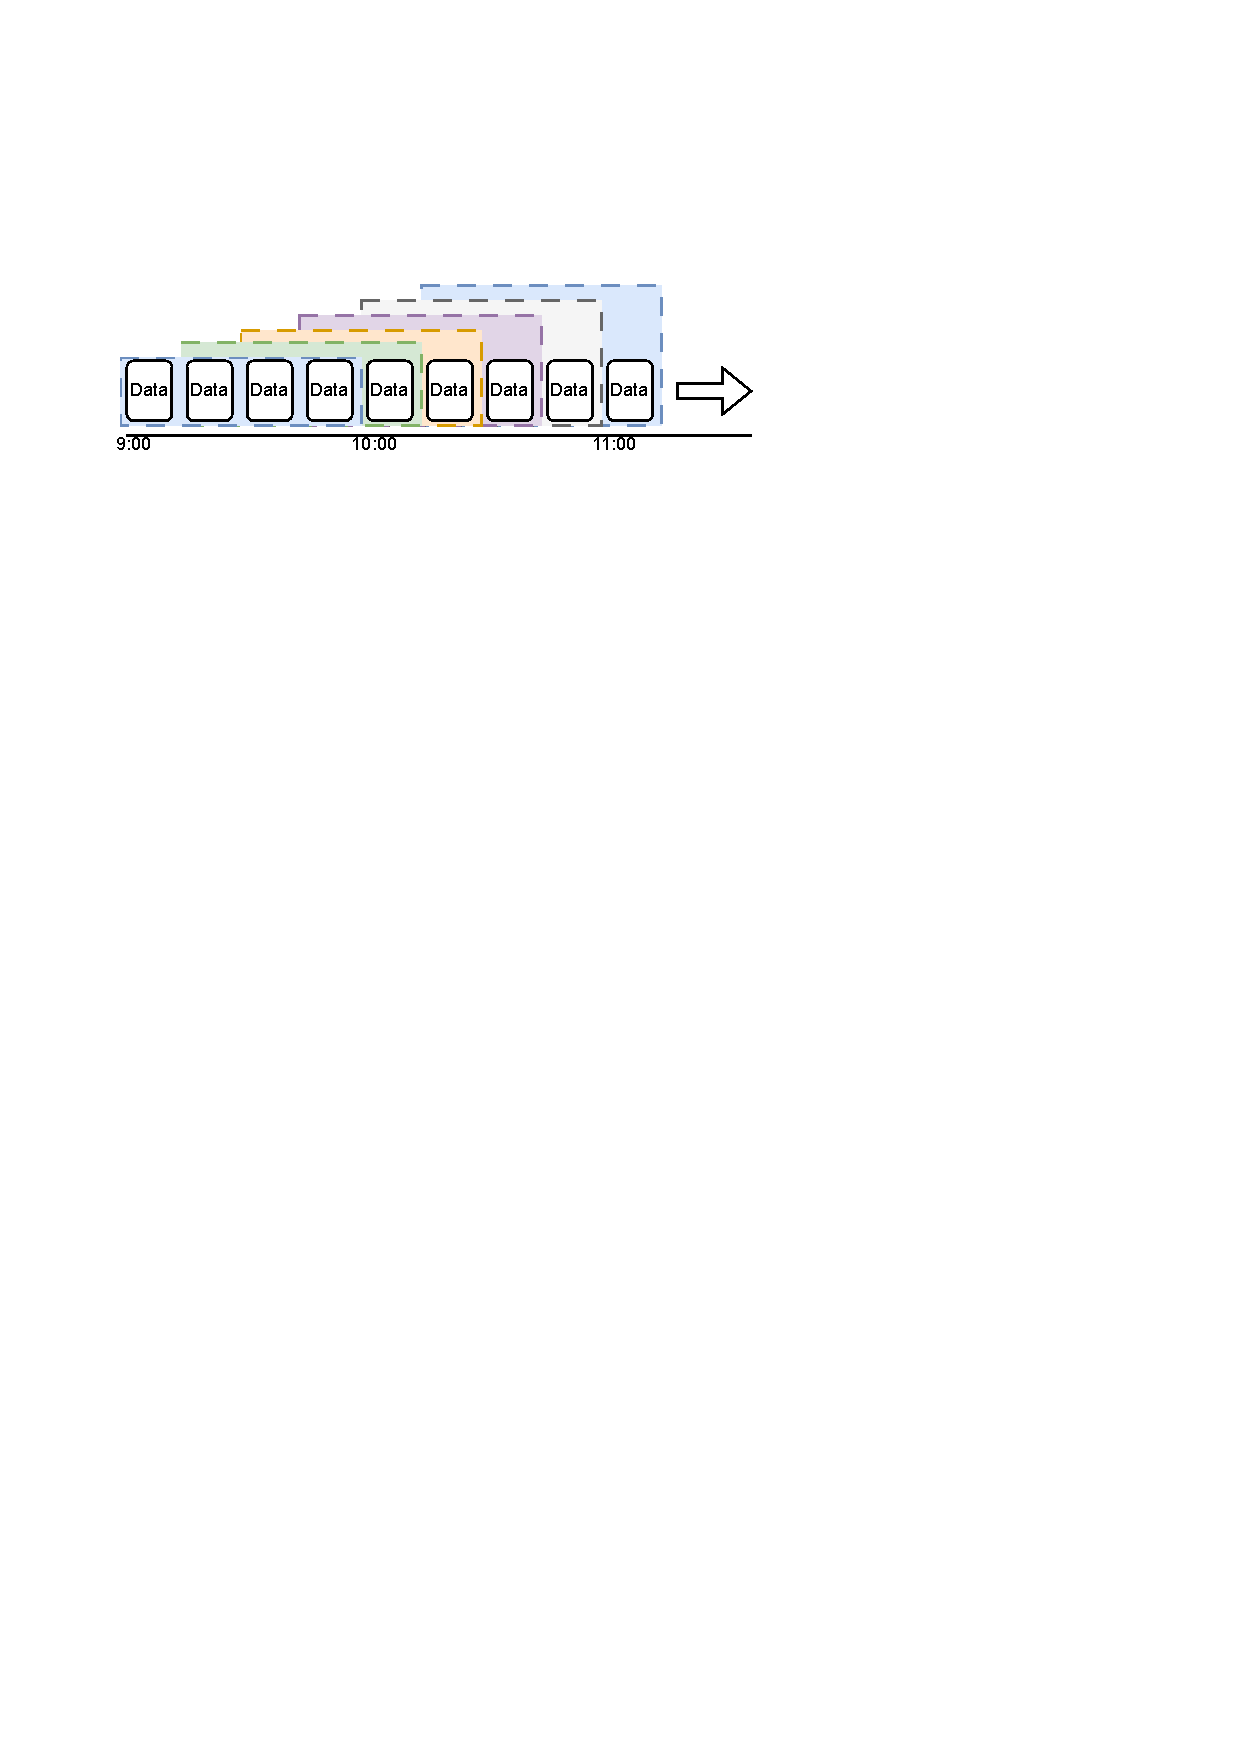
\includegraphics[width=1\textwidth]{figures/sliding-window.pdf}
    \caption{Sliding-window aggregation on the last 1 hour's data}
    \label{fig_sliding_window}
\end{figure}

\begin{figure}[H]
    \centering
    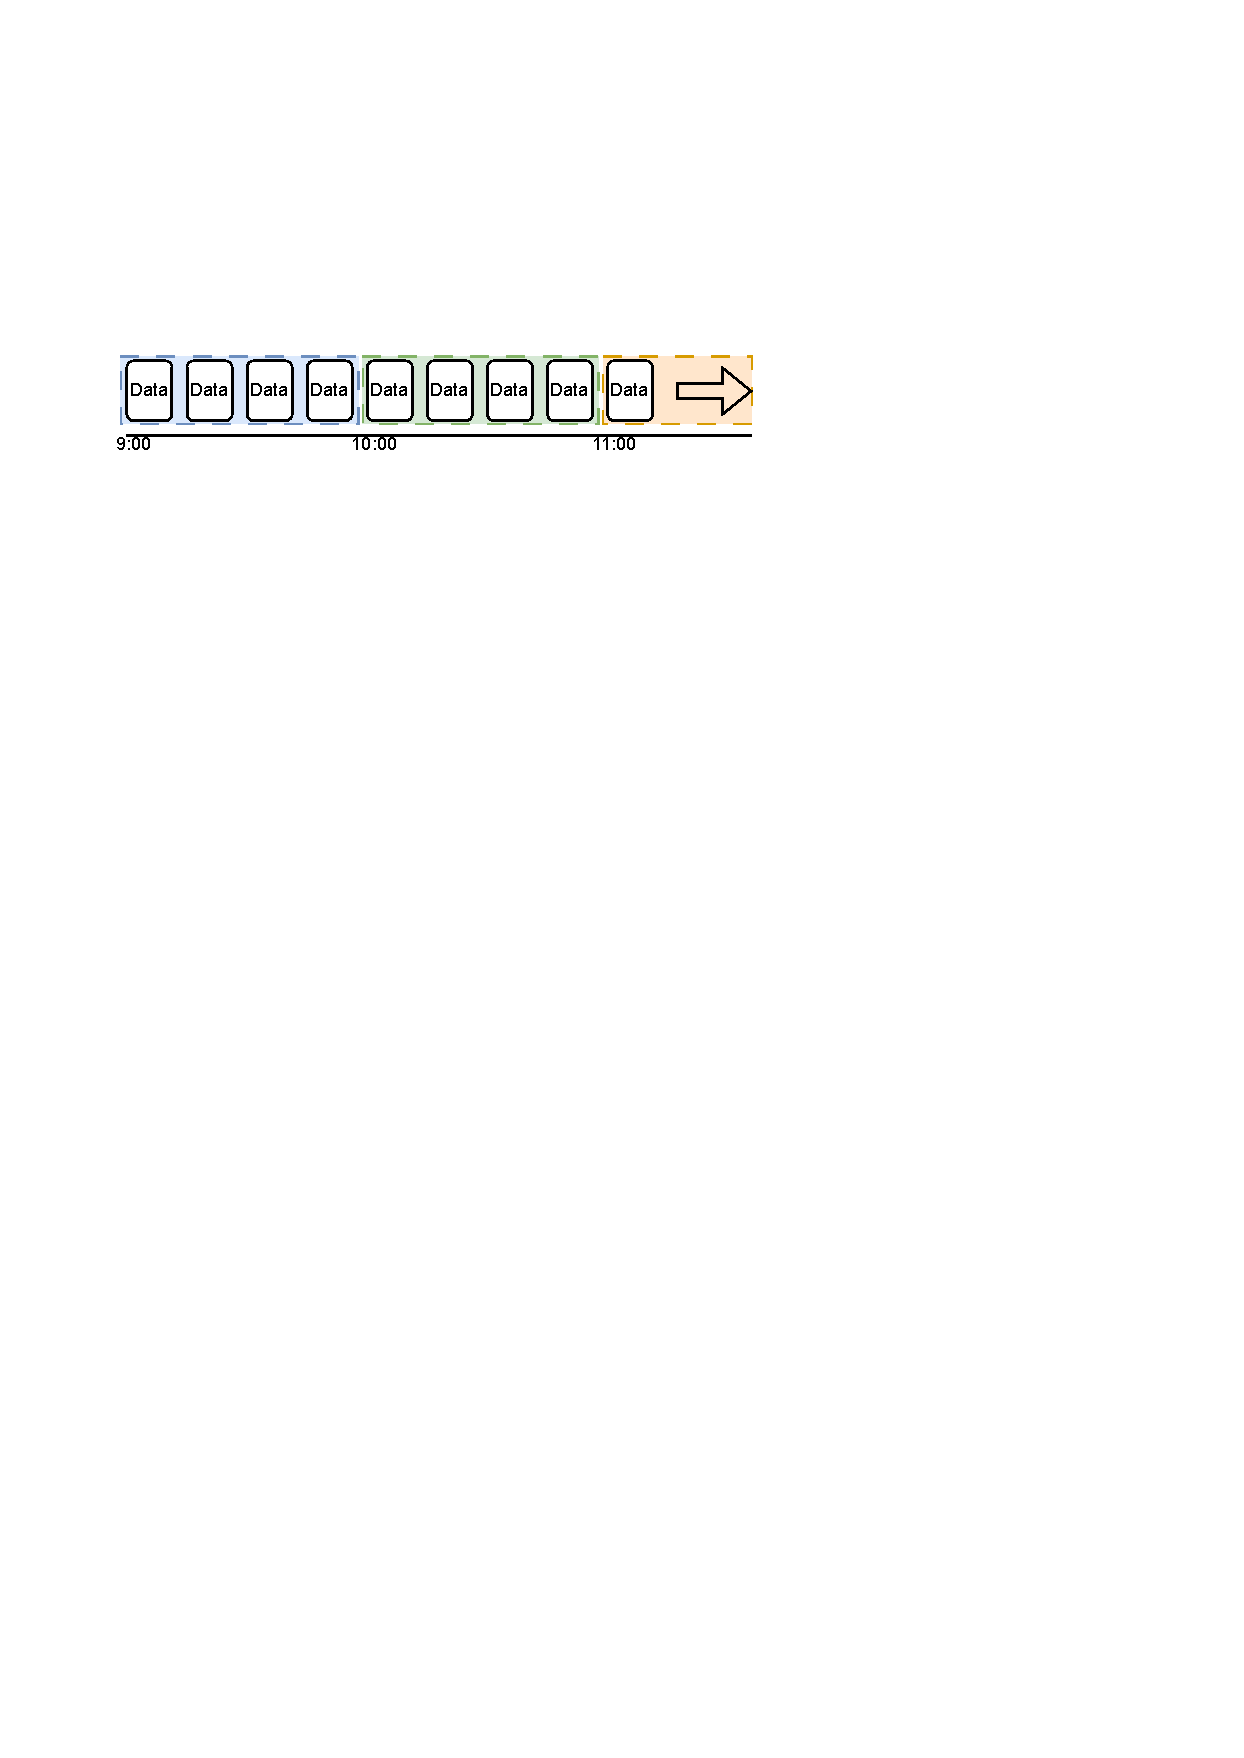
\includegraphics[width=1\textwidth]{figures/fixed-sliding-window.pdf}
    \caption{Aggregation with a fixed start time}
    \label{fig_fixed_sliding_window}
\end{figure}

We need to benchmark all four design choices to reach a final decision, which will be further discussed in Subsection \ref{subsec:performance}.

% The triggers with an in-memory aggregates approach leverage in-memory processing capabilities to analyze GPU metrics in real-time. This involves maintaining an in-memory cache of aggregated metrics and facilitating rapid alerting based on live data without continuous queries to the time-series database. The in-memory cache balances real-time responsiveness and resource efficiency in the alerting system.

The \textbf{API design} of the Timescale Alert is as follows, which provides the data for other services and allows easier integration:

\begin{itemize}
    \item \textbf{/version}: Same as Timescale Ingest, it displays the version information and build time.
    \item \textbf{/healthStatus}: Checking connection status between the timescale ingest and the database.
    \item \textbf{/dismiss/:host/:job/:gpu}: Disable or enable the alert for the specified GPU on the host from a specific job ID.
    \item \textbf{/history}: Displaying a list of JSON objects or a table that shows the alert history. It can be filtered by the host, username, job ID, and type.
    \item \textbf{/}: Displaying the current alert status. Host, username, and job ID can also be the filter.
\end{itemize}

Below is an example showing the GPU alert history output section of the modified \texttt{seff} command we added for Timescale Alert. The alert information is printed via the above-mentioned \texttt{/history} endpoint. Here are a few alert histories related to GPU usage. Each entry shows the time when the alert happened, the hostname, and the GPU ID that generated the alert event. It also shows the 75th percentile aggregation result for the sliding window time frame that contributes to the alert status change, and the \texttt{Normal} column shows whether this entry generates a new alert (with \texttt{x}) or clears the old alert (with \texttt{v}).

\begin{lstlisting}
$ seff 5465
GPU Alert History
-------------------------------------------------------------------
GPU Usage
                     Time   Hostname   GPU Id   75% (%)   Normal
2024-04-25T17:05:55+03:00     r14g04        2        5      x
2024-04-25T17:06:41+03:00     r14g04        2       21      v
2024-04-25T17:10:49+03:00     r14g05        1        8      x
2024-04-25T17:11:17+03:00     r14g05        1       23      v
-------------------------------------------------------------------
\end{lstlisting}

\section{Alert dashboard}

The alert dashboard reads data to display and learn about the current job status. It renders tables through the web page to internal users, such as CSC user support experts. As shown in Figure \ref{fig_status_dashboard}, the dashboard has a counter for the viewers to know the total number of GPUs in use, and how many are currently on alert. 

\begin{figure}[H]
    \centering
    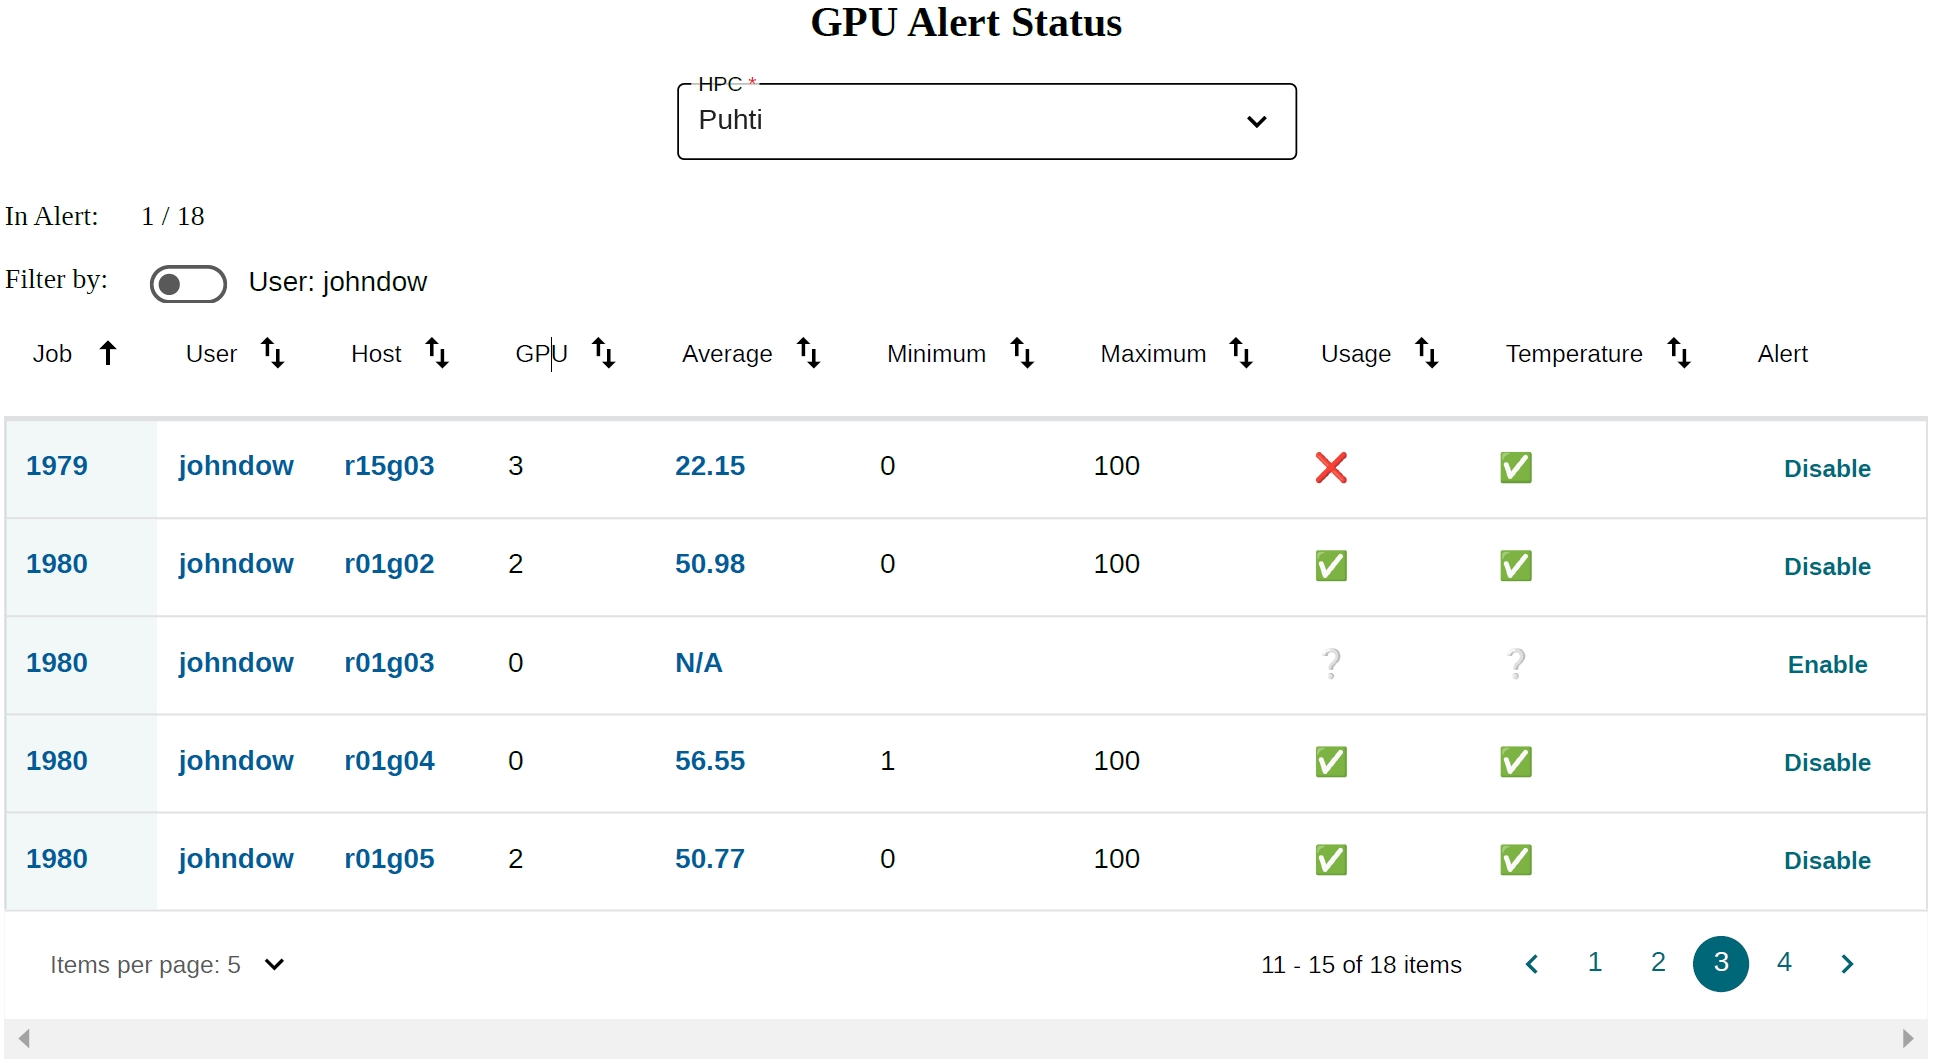
\includegraphics[width=1.1\textwidth]{figures/status-dashboard.png}
    \caption{GPU alert status dashboard}
    \label{fig_status_dashboard}
\end{figure}

In addition, the dashboard allows users to disable or re-enable job alerts, so that admins can improve the alert manually and focus more on those jobs, that have not been checked or can be improved. The users can also click on the button to check more detailed JSON information about jobs from the output of \texttt{sacct --json}. (We don't render that information directly into the table, since the SQL database behind Slurm runs full steam for several seconds when calling that, even for a single job)

Besides showing the alert status, the dashboard also displays the watermark information for the job lifetime metrics, such as the average, minimum, and maximum GPU load, to give admins a whole picture of what might happen to the job.

Aside from sorting the data, the dashboard allows the viewers to filter the data by job ID, user name, hostname, and alert status, so viewers can quickly target different entities in question. When we filter by user name or job ID, the dashboard also allows admins to send emails to the user in question, with one click, from the preset template, for the current jobs in the alert. One example email generated by the dashboard, when we click the button in Figure \ref{fig_status_dashboard}, is as follows:

\begin{minted}[breaklines,
frame=lines,
framesep=2mm,
baselinestretch=1.2,
fontsize=\footnotesize,
breaksymbolleft=]{text}
To: johndow@users.csc.fi
Subject: Low GPU utilization rate with the job you are running on Puhti

Dear johndow,

We have noticed that you have a low utilization rate, at least during the last 30 min, according to our monitoring system, for the jobs you are running on Puhti:

- GPU 0 on host r03g03 for job 21850954, with lifetime average 3.13%, maximum 20%, miminum 0%.

Please review them and make improvements at your earliest convenience. We recommend checking your job scripts and programs to ensure that the jobs are running as intended.

You might also want to consider the following:
1. Running "seff <job_id>" on the login node to check the job's resource usage.
2. Find out the history of the job's GPU data by visiting: https://puhti-ood-testing.csc.fi/pun/sys/dashboard/custom/job_monitor
3. Check the job's output and error logs for any error messages.
4. Reduce the number of GPUs requested in your job script.

if the situation continues and we receive no response from you, we might take actions to ensure fair usage for all our users. Thank you for your cooperation! If you have any questions or need help, please feel free to contact us!

Best regards,
CSC computing services
\end{minted}

We also have a dashboard showing the alert history, as presented in Figure \ref{fig_history_dashboard}, which shows the alert status change time, job ID, user name, hostname, GPU ID, alert type, alert value (for usage alert, it will be the 75\% percentile), and whether the status change generates a new alert or clear out an old one. The history dashboard also shares the same features as the status dashboard.

\begin{figure}[H]
    \centering
    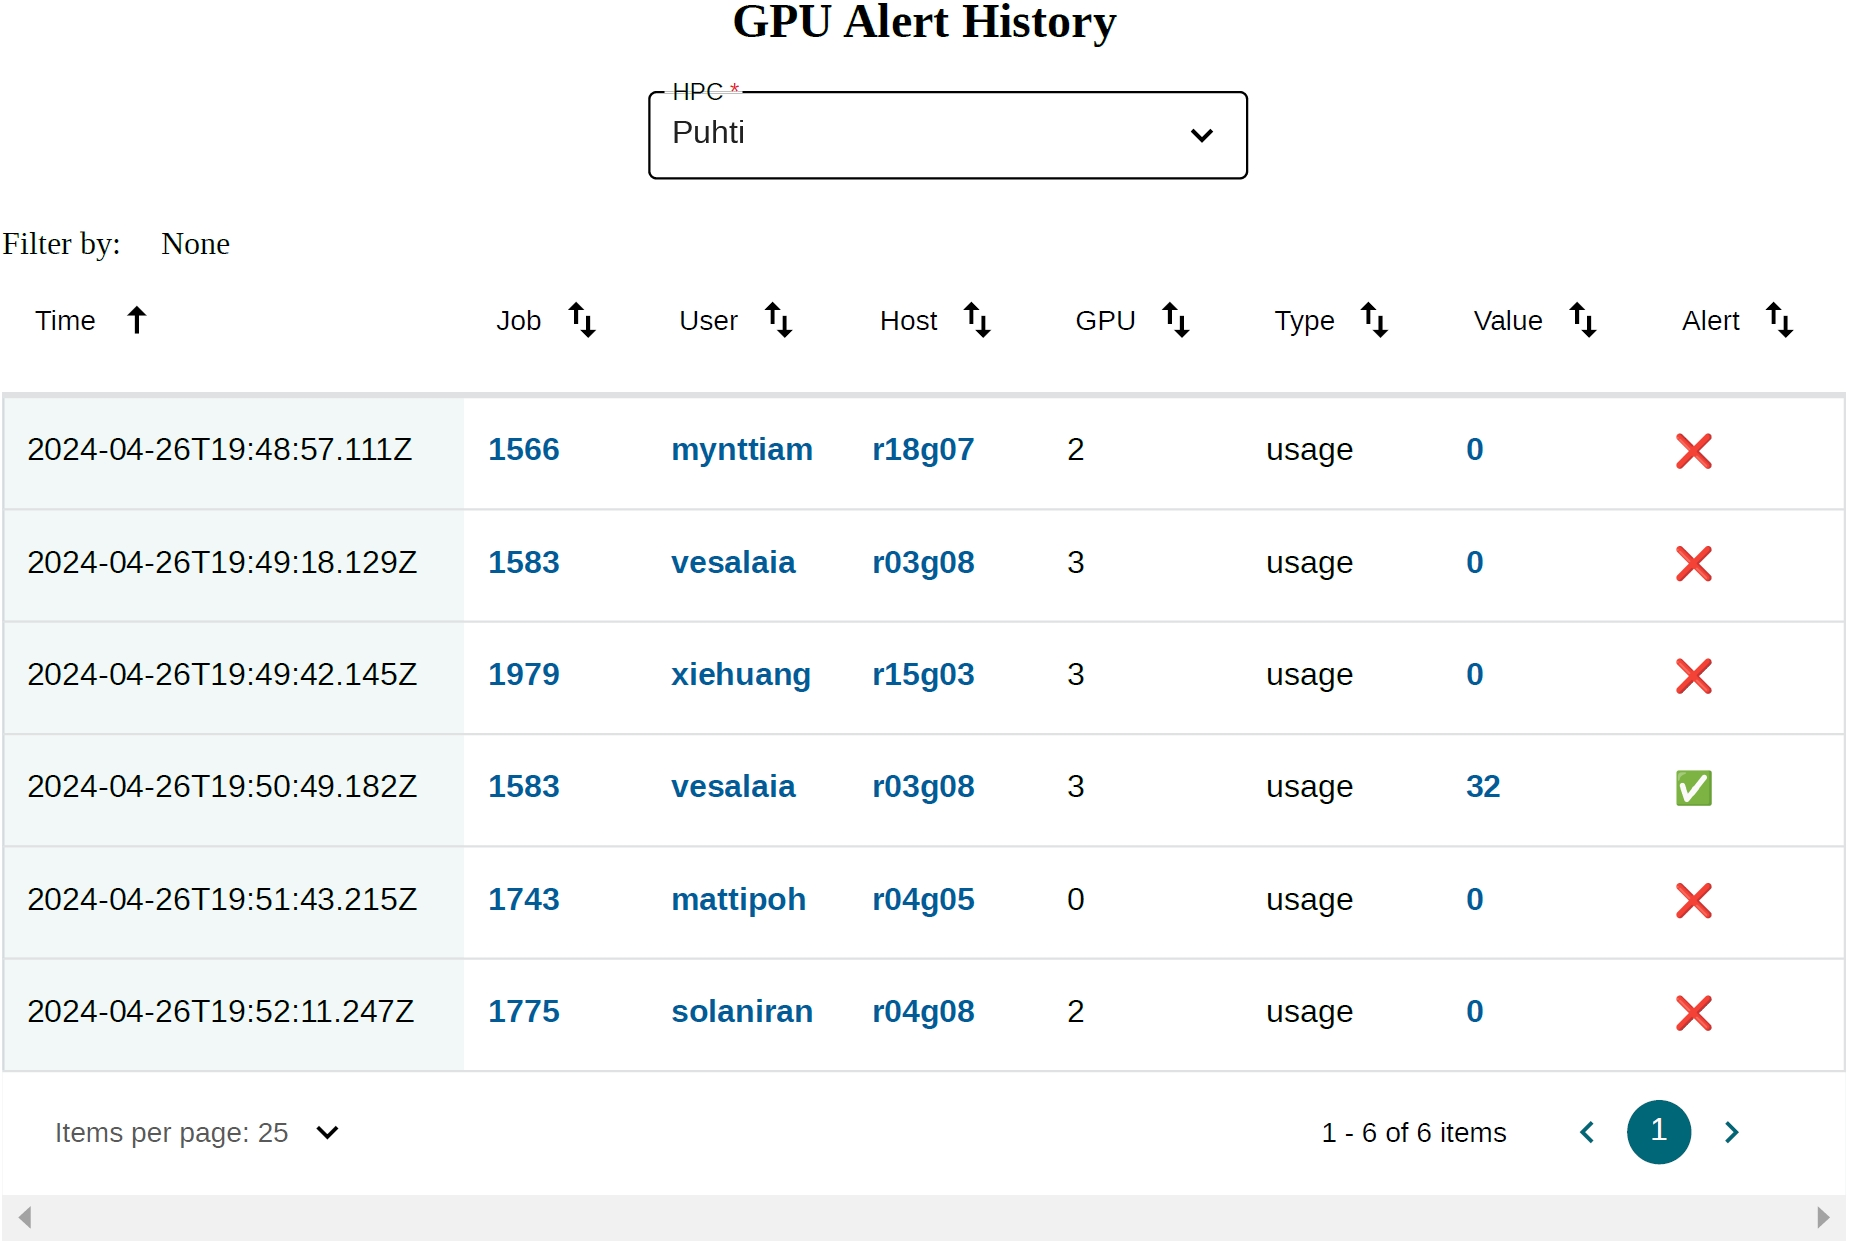
\includegraphics[width=1.1\textwidth]{figures/history-dashboard.png}
    \caption{GPU alert history dashboard}
    \label{fig_history_dashboard}
\end{figure}
